\documentclass[a4paper,11pt,twoside]{book}
\usepackage[top=3cm,bottom=3cm,left=2cm,right=2cm]{geometry}
\usepackage{footnote}
\usepackage{amsbsy}
\usepackage{graphicx}
\usepackage{longtable}
\usepackage{fancyhdr}
\usepackage[T1]{fontenc} % important for having searchable underscores
\usepackage{bm}
\usepackage[sort&compress,numbers]{natbib}
%\usepackage{fancyheadings}
%\setlength{\parindent}{0in}
%\setlength{\parskip}{0.05in}
\setlength{\parskip}{0.1in}


%\usepackage{a4wide}
\usepackage{color}
\def\red{\textcolor{red}}       %
\def\old#1{\textcolor{red}{#1}}
\def\new#1{\textcolor{blue}{#1}}

\usepackage{amsmath}


% Print only chapters in the Table Of Contents
\setcounter{tocdepth}{0} 


%\parskip=2mm

% Ensure that blank pages don't have numbers or heading on them 
\makeatletter
\def\cleardoublepage{\clearpage\if@twoside \ifodd\c@page\else
 \hbox{}
 \vspace*{\fill}
 \thispagestyle{empty}
 \newpage\fi\fi}
\makeatother

% set fancy headings
\pagestyle{fancy}
\lhead[{\it \thepage}]{{\bf\it {\tt wannier90}: User Guide}}
\chead{}
\rhead[{\bf\it {\tt wannier90}: User Guide}]{{\it \thepage}}
\renewcommand{\headrulewidth}{0.2pt}
\lfoot{}
\cfoot{}
\rfoot{}
\renewcommand{\footrulewidth}{0pt}
\setlength{\footskip}{0.25in}
\setlength{\parindent}{0in}


%% This part slightly modifies the default definition of \chapter
%% (found in book.cls) to add a \hspace{2em} before numbered chapters.
\makeatletter
\def\@chapter[#1]#2{\ifnum \c@secnumdepth >\m@ne
                       \if@mainmatter
                         \refstepcounter{chapter}%
                         \typeout{\@chapapp\space\thechapter.}%
                         \addcontentsline{toc}{chapter}%
                                   {\hspace{2em}\protect\numberline{\thechapter}#1}%
                       \else
                         \addcontentsline{toc}{chapter}{#1}%
                       \fi
                    \else
                      \addcontentsline{toc}{chapter}{#1}%
                    \fi
                    \chaptermark{#1}%
                    \addtocontents{lof}{\protect\addvspace{10\p@}}%
                    \addtocontents{lot}{\protect\addvspace{10\p@}}%
                    \if@twocolumn
                      \@topnewpage[\@makechapterhead{#2}]%
                    \else
                      \@makechapterhead{#2}%
                      \@afterheading
                    \fi}
\makeatother

\title{{\tt wannier90}: User Guide}

\author{Version 2.1.0}

\date{13th January 2017}
%\date{\color{red} \today}


%%% THIS SHOULD BE THE LAST PACKAGE TO BE LOADED!
%hidelinks to remove colored borders from links
%plainpages=false needed for the unnumbered pages
%breaklinks=true to allow to break long links (e.g. long titles) on
%more than one line
%bookmarksopen open the bookmarks in the adobe reader plugin
%bookmarksopenlevel decide the max level at which the bookmarks should
%be open
% pdfdisplaydoctitle=true to show the document title instead of the
% filename in the titlebar of adobereader
\usepackage[plainpages=false,breaklinks=true,pdfborder=0 0 0,pdfdisplaydoctitle=true,bookmarksopen=true,bookmarksopenlevel=0,pdftex,%
%Comment next line if it makes problems
%(it requires a recent LaTeX distribution)
            hidelinks,
            pdftitle={Wannier90 User Guide},
            pdfkeywords={wannier90;postw90;pwscf;user guide}]{hyperref}

\begin{document}
\newcommand{\wannier}{\texttt{wannier90}}
\newcommand{\postw}{\texttt{postw90}}
\newcommand{\bw}{\texttt{BoltzWann}}
\newcommand{\pwscf}{\textsc{pwscf}}
\newcommand{\QE}{\textsc{quantum-espresso}}
\newcommand{\Mkb}{\mathbf{M}^{(\mathbf{k},\mathbf{b})}}
\newcommand{\Ak}{\mathbf{A}^{(\mathbf{k})}}
\newcommand{\Uk}{\mathbf{U}^{(\mathbf{k})}}
\newcommand{\cond}{\item[$\star$]}
\newcommand{\omi}{\Omega_{\mathrm{I}}}
\newcommand{\omt}{\widetilde{\Omega}}
\newcommand{\bvec}[1]{\bm{\mathrm{#1}}}

\maketitle

\tableofcontents

%\listoftables

%\listoffigures

\part{Introduction}

\chapter{Introduction}

\section{Methodology}
Wannier90 computes Maximally Localised
Wannier Functions (MLWFs) following the method of Marzari and Vanderbilt (MV).\footnote{
{\it Maximally localized generalized Wannier functions for composite energy bands}
N. Marzari and D. Vanderbilt, Phys. Rev. B 56, 12847 (1997)}
For entangled energy bands  the method of
Souza, Marzari and Vanderbilt (SMV)\footnote{{\it Maximally localized
    Wannier functions for entangled energy bands} 
I. Souza, N. Marzari and D. Vanderbilt, Phys. Rev. B 65, 035109 (2002)}
is used.
We briefly introduce the methods and key definitions, but full details
can be found in the original papers. 

First principles codes typically solve the electronic structure of
periodic materials in terms of Bloch states, $\psi_{n{\bf k}}$. 
These extended states are characterised by a band index $n$ and crystal
momentum ${\bf k}$. An alternative representation can be given in terms
of spatially localised functions known as Wannier functions (WFs). The WF 
centred on a lattice site ${\bf R}$,  $w_{n{\bf R}}({\bf r})$, 
is written in terms of the set of Bloch states as
\begin{equation}
w_{n{\bf R}}({\bf r})=\frac{V}{(2\pi)^3}\int_{BZ} \left[\sum_{m} U^{({\bf
k})}_{mn} \psi_{m{\bf k}}({\bf r})\right]e^{-\mathrm{i}{\bf k}.{\bf R}} d{\bf k},
\end{equation}
where $\bf{U}^{({\bf k})}$ is a unitary matrix that mixes the Bloch
states at each 
${\bf k}$. $\bf{U}^{({\bf k})}$ is not uniquely defined and different choices
will lead to WFs with varying spatial localisations. We define the
spread $\Omega$
of the WFs as 
\begin{equation}
\Omega=\sum_n \left[\langle w_{n{\bf 0}}({\bf r})| r^2 | w_{n{\bf
      0}}({\bf r}) \rangle - | \langle w_{n{\bf 0}}({\bf r})| {\bf r} | w_{n{\bf
      0}}({\bf r}) \rangle |^2 \right].
\end{equation}
The total spread can be decomposed into a gauge invariant term
$\Omega_{\rm I}$ plus a term ${\tilde \Omega}$ that is dependant on the gauge
choice $\bf{U}^{({\bf k})}$. ${\tilde \Omega}$ can
be further divided into terms diagonal and off-diagonal in the WF basis,
$\Omega_{\rm D}$ and $\Omega_{\rm OD}$.
\begin{equation}
\Omega=\Omega_{\rm I}+{\tilde \Omega}=\Omega_{\rm I}+\Omega_{\rm D}+\Omega_{\rm OD}
\end{equation}
where
\begin{equation}
\Omega_{{\rm I}}=\sum_n \left[\langle w_{n{\bf 0}}({\bf r})| r^2 | w_{n{\bf
      0}}({\bf r}) \rangle - \sum_{{\bf R}m} \left| \langle w_{n{\bf R}}({\bf r})| {\bf r} | w_{n{\bf
      0}}({\bf r}) \rangle \right| ^2 \right]
\end{equation}
\begin{equation}
\Omega_{\rm D}=\sum_n \sum_{{\bf R}\neq{\bf 0}} |\langle w_{n{\bf R}}({\bf r})| {\bf r} |
w_{n{\bf 0}}({\bf r}) \rangle|^2 
\end{equation}
\begin{equation}
\Omega_{\rm OD}=\sum_{m\neq n} \sum_{{\bf R}} |\langle w_{m{\bf R}}({\bf
  r})| {\bf r} |
w_{n{\bf 0}}({\bf r}) \rangle |^2 
\end{equation}
The MV method minimises the gauge dependent spread $\tilde{\Omega}$ with respect the set
of $\bf{U}^{({\bf k})}$ to obtain MLWFs.

The Wannier90 code requires two ingredients from an initial electronic structure calculation.
\begin{enumerate}
\item The overlaps between the cell periodic part of the Bloch states $|u_{n{\bf k}}\rangle$ 
\begin{equation}
M_{mn}^{(\bf{k,b})}=\langle u_{m{\bf k}}|u_{n{\bf k}+{\bf b}}\rangle,
\end{equation}
where the vectors ${\bf b}$, which connect a given k-point with its neighbours, are determined
by the Wannier90 code according to the prescription outlined in MV.
\item As a starting guess the projection of the Bloch states
  $|\psi_{n\bf{k}}\rangle$ onto trial localised orbitals $|g_{n}\rangle$ 
\begin{equation}
A_{mn}^{(\bf{k})}=\langle \psi_{m{\bf k}}|g_{n}\rangle,
\end{equation}
\end{enumerate}
Note that $\bf{M}^{(\bf{k,b})}$, $\bf{A}^{(\bf{k})}$ and
$\bf{U}^{({\bf k})}$ are all 
small, $N_{{\rm wann}}\times N_{{\rm wann}}$ matrices, independent of
the basis set used to obtain the original Bloch states.  

To date the Wannier90 code has been
used in combination with electronic codes based on plane-waves and
pseudopotentials (norm-conserving and ``ultrasoft'') as well as mixed
basis set techniques such as FLAPW. 

\subsection{Entangled Energy Bands}
The above description is sufficient to obtain Wannier functions for an
isolated set of bands, such as the valence states in an insulator. In
order to obtain MLWFs for entangled energy bands we use the
``disentanglement'' procedure introduced in SMV.

We define an energy window (the ``outer window''). At a given
k-point $\bf{k}$, 
$N^{{\bf k}}_{{\rm win}}$ states lie within this energy window. We
obtain a set of 
$N_{{\rm wann}}$ Bloch states by performing a unitary
transformation amongst the Bloch states which fall within the energy window at each k-point:
 \begin{equation}
| u_{n{\bf k}}^{{\rm opt}}\rangle = \sum_{m\in N^{{\bf k}}_{{\rm win}}}
U^{{\rm dis}({\bf k})}_{mn} | u_{m{\bf k}}\rangle
\end{equation}
where $\bf{U}^{{\rm dis}({\bf k})}$ is a rectangular $N_{{\rm
 wann}}\times N^{{\bf k}}_{{\rm win}}$
 matrix\footnote{As
    $\bf{U}^{{\rm dis}({\bf k})}$ is a rectangular matrix this is a unitary
    operation in the sense that $(\bf{U}^{{\rm dis}({\bf k})})^{\dagger}\bf{U}^{{\rm dis}({\bf k})}=\bf{1}$.}. The set of $\bf{U}^{{\rm dis}({\bf k})}$ are obtained by minimising
 the gauge invariant spread $\Omega_{{\rm I}}$ within the outer energy
 window. The MV procedure can then be used to minimise $\tilde{\Omega}$
 and hence obtain MLWF for this optimal subspace.

It should be noted that the energy bands of this
optimal subspace may not correspond to any of the original energy
bands (due to mixing between states). In order to preserve exactly the
properties of a system in a given energy range (eg, around the Fermi
level) we introduce a second  energy window. States lying
within this inner, or ``frozen'', energy window are included unchanged
in the optimal subspace.

\subsection{Citation}
We ask that you acknowledge the use of Wannier90 in any publications
arising from the use of this code through the following reference
\begin{quote}
[ref] A. A. Mostofi, J. R. Yates,
N. Marzari, I. Souza and D. Vanderbilt,  

 http://www.wannier.org/                 
\end{quote}                                                              

It would also be appropriate to cite the original articles:\\\\
{\it Maximally localized generalized Wannier functions for composite energy bands}\\
N. Marzari and D. Vanderbilt, Phys. Rev. B 56, 12847 (1997)\\\\
{\it Maximally localized Wannier functions for entangled energy bands}\\
I. Souza, N. Marzari and D. Vanderbilt, Phys. Rev. B 65, 035109 (2002)


\subsection{Credits}
The present release of Wannier90 was written by Arash Mostofi (Marzari
group @ MIT) and Jonathan Yates (Souza Group @ UCB/LBNL). Wannier90 is
based on routines written in 1996-7 for occupied bands by Nicola Marzari
and David Vanderbilt and for entangled bands by Ivo Souza, Nicola Marzari,
and David Vanderbilt in 2000-1. 

Acknowledgements: ?

Wannier90 \copyright 1997-2006 Jonathan Yates, Arash
Mostofi, Nicola Marzari, Ivo Souza, David Vanderbilt      

\subsection{Licence}
All the material in this distribution is free software; you can
redistribute it and/or 
modify it under the terms of the GNU General Public License
as published by the Free Software Foundation; either version 2
of the License, or (at your option) any later version.

This program is distributed in the hope that it will be useful,
but WITHOUT ANY WARRANTY; without even the implied warranty of
MERCHANTABILITY or FITNESS FOR A PARTICULAR PURPOSE.  See the
GNU General Public License for more details.

You should have received a copy of the GNU General Public License
along with this program; if not, write to the Free Software
Foundation, Inc., 51 Franklin Street, Fifth Floor, Boston, MA  02110-1301, USA.


 


\part{\texttt{wannier90.x}\label{part:w90}}

\chapter{Methodology}\label{sec:method}
\wannier\ computes maximally-localised Wannier functions (MLWF)
following the method of Marzari and Vanderbilt (MV)~\cite{MV}.
For entangled energy bands, the method of Souza, Marzari and
Vanderbilt (SMV)~\cite{SMV} is used. We introduce briefly the methods
and key definitions here, but full details can be found in the
original papers and in Ref.~\cite{W90}.

First-principles codes typically solve the electronic structure of
periodic materials in terms of Bloch states, $\psi_{n{\bf k}}$. 
These extended states are characterised by a band index $n$ and crystal
momentum ${\bf k}$. An alternative representation can be given in terms
of spatially localised functions known as Wannier functions (WF). The WF 
centred on a lattice site ${\bf R}$, $w_{n{\bf R}}({\bf r})$, 
is written in terms of the set of Bloch states as
\begin{equation}
w_{n{\bf R}}({\bf r})=\frac{V}{(2\pi)^3}\int_{\mathrm{BZ}}
\left[\sum_{m} U^{({\bf k})}_{mn} \psi_{m{\bf k}}({\bf
    r})\right]e^{-\mathrm{i}{\bf k}.{\bf R}} \:\mathrm{d}{\bf k} \ , 
\end{equation}
where $V$ is the unit cell volume, the integral is over the Brillouin
zone (BZ), and $\Uk$ is a unitary matrix that mixes the Bloch 
states at each ${\bf k}$. $\Uk$ is not uniquely defined and different
choices will lead to WF with varying spatial localisations. We define
the spread $\Omega$ of the WF as 
\begin{equation}
\Omega=\sum_n \left[\langle w_{n{\bf 0}}({\bf r})| r^2 | w_{n{\bf
      0}}({\bf r}) \rangle - | \langle w_{n{\bf 0}}({\bf r})| {\bf r}
      | w_{n{\bf 0}}({\bf r}) \rangle |^2 \right].
\end{equation}
The total spread can be decomposed into a gauge invariant term
$\Omega_{\rm I}$ plus a term ${\tilde \Omega}$ that is dependant on the gauge
choice $\Uk$. ${\tilde \Omega}$ can
be further divided into terms diagonal and off-diagonal in the WF basis,
$\Omega_{\rm D}$ and $\Omega_{\rm OD}$,
\begin{equation}
\Omega=\Omega_{\rm I}+{\tilde \Omega}=\Omega_{\rm I}+\Omega_{\rm
  D}+\Omega_{\rm OD} 
\end{equation}
where
\begin{equation}
\Omega_{{\rm I}}=\sum_n \left[\langle w_{n{\bf 0}}({\bf r})| r^2 | w_{n{\bf
      0}}({\bf r}) \rangle - \sum_{{\bf R}m} \left| \langle w_{n{\bf
      R}}({\bf r})| {\bf r} | w_{n{\bf 0}}({\bf r}) \rangle \right| ^2
      \right] 
\end{equation}
\begin{equation}
\Omega_{\rm D}=\sum_n \sum_{{\bf R}\neq{\bf 0}} |\langle w_{n{\bf
    R}}({\bf r})| {\bf r} | w_{n{\bf 0}}({\bf r}) \rangle|^2 
\end{equation}
\begin{equation}
\Omega_{\rm OD}=\sum_{m\neq n} \sum_{{\bf R}} |\langle w_{m{\bf R}}({\bf
  r})| {\bf r} | w_{n{\bf 0}}({\bf r}) \rangle |^2 
\end{equation}
The MV method minimises the gauge dependent spread $\tilde{\Omega}$
with respect the set of $\Uk$ to obtain MLWF.

\wannier\ requires two ingredients from an initial electronic
structure calculation. 
\begin{enumerate}
\item The overlaps between the cell periodic part of the Bloch states
  $|u_{n{\bf k}}\rangle$  
\begin{equation}
M_{mn}^{(\bf{k,b})}=\langle u_{m{\bf k}}|u_{n{\bf k}+{\bf b}}\rangle,
\end{equation}
where the vectors ${\bf b}$, which connect a given k-point with its
neighbours, are determined 
by \wannier\ according to the prescription outlined in Ref.~\cite{MV}.
\item As a starting guess the projection of the Bloch states
  $|\psi_{n\bf{k}}\rangle$ onto trial localised orbitals $|g_{n}\rangle$ 
\begin{equation}
A_{mn}^{(\bf{k})}=\langle \psi_{m{\bf k}}|g_{n}\rangle,
\end{equation}
\end{enumerate}
Note that $\Mkb$, $\Ak$ and $\Uk$ are all small, $N \times
N$ matrices\footnote{Technically, this is true for the case of an
  isolated group of $N$ bands from which we obtain $N$ MLWF. When
  using the disentanglement procedure of Ref.~\cite{SMV}, $\Ak$, for
  example, is a rectangular matrix. See Section~\ref{sec:disentangle}.}
that are independent of the basis set used to obtain the original
Bloch states.

To date, \wannier\ has been used in combination with electronic codes
based on plane-waves and pseudopotentials (norm-conserving and
ultrasoft~\cite{USPP}) as well as mixed basis set techniques such as
FLAPW~\cite{MnO}.

\section{Entangled Energy Bands}\label{sec:disentangle}
The above description is sufficient to obtain MLWF for an
isolated set of bands, such as the valence states in an insulator. In
order to obtain MLWF for entangled energy bands we use the
``disentanglement'' procedure introduced in Ref.~\cite{SMV}.

We define an energy window (the ``outer window''). At a given
k-point $\bf{k}$, $N^{({\bf k})}_{{\rm win}}$ states lie within this
energy window. We obtain a set of $N$ Bloch states by
performing a unitary transformation amongst the Bloch states which
fall within the energy window at each k-point: 
 \begin{equation}
| u_{n{\bf k}}^{{\rm opt}}\rangle = \sum_{m\in N^{({\bf k})}_{{\rm win}}}
U^{{\rm dis}({\bf k})}_{mn} | u_{m{\bf k}}\rangle
\end{equation}
where $\bf{U}^{{\rm dis}({\bf k})}$ is a rectangular $N \times N^{({\bf k})}_{{\rm win}}$
 matrix\footnote{As $\bf{U}^{{\rm dis}({\bf k})}$ is a rectangular
 matrix this is a unitary operation in the sense that $(\bf{U}^{{\rm
 dis}({\bf k})})^{\dagger}\bf{U}^{{\rm dis}({\bf k})}=\bf{1}$.}. The
 set of $\bf{U}^{{\rm dis}({\bf k})}$ are obtained by minimising 
 the gauge invariant spread $\Omega_{{\rm I}}$ within the outer energy
 window. The MV procedure can then be used to minimise $\tilde{\Omega}$
 and hence obtain MLWF for this optimal subspace.

It should be noted that the energy bands of this optimal subspace may
not correspond to any of the original energy bands (due to mixing
between states). In order to preserve exactly the properties of a
system in a given energy range (e.g., around the Fermi level) we
introduce a second  energy window. States lying within this inner, or
``frozen'', energy window are included unchanged in the optimal
subspace.


\chapter{Parameters}\label{chap:parameters}

\section{Usage}
{\tt
\begin{quote}
wannier90.x [-pp] [seedname]
\end{quote} }
\begin{itemize}
\item{ {\tt seedname}: If a seedname string is given the code will read its input
from a file {\tt seedname.win}. The default value is {\tt wannier}.}
\item { {\tt -pp}: This optional flag tells the code to generate
a list of the required overlaps and then exit. 
This information is written to the file {\tt seedname.nnkp}.}
\end{itemize}

\section{{\tt seedname.win} File}
The \wannier\ input file {\tt seedname.win} has a flexible free-form
structure. 

The ordering of the keywords is not significant. Case is ignored (so
\verb#num_bands# is the same as \verb#Num_Bands#). Characters after !, or \#
are treated as comments. Most keywords have a default value that is
used unless the keyword is given in {\tt seedname.win}. Keywords can be set
in any of the following ways
{\tt
\begin{quote}
num\_wann   4

num\_wann = 4

num\_wann : 4
\end{quote} }
A logical keyword can be set to {\tt .true.} using any of the following
strings: {\tt T}, {\tt true}, {\tt .true.}.

For further examples see Section~\ref{winfile} and the the \wannier\ Tutorial.


\section{Keyword List}
\label{parameter_data}

\begin{table}
\begin{center}
\begin{tabular}{|c|c|p{6cm}|}
\hline
Keyword & Type & Description \\
        &      &             \\
\hline\hline
\multicolumn{3}{|c|}{System Parameters} \\
\hline
{\sc num\_wann }   & I & Number of WF \\
{\sc num\_bands }   & I & Number of bands passed to the code \\
{\sc unit\_cell\_cart }   & P & Unit cell vectors in Cartesian coordinates \\
{\sc atoms\_cart }*   & P & Positions of atoms in Cartesian coordinates \\
{\sc atoms\_frac }*   & R & Positions of atoms in fractional
coordinates with respect to the lattice vectors \\
{\sc mp\_grid }   & I & Dimensions of the Monkhorst-Pack grid of
k-points \\
%{\sc mp\_grid\_automatic }**   & L & Determine the k-point automatically \\
{\sc kpoints }   & R & List of k-points in the Monkhorst-Pack grid \\
{\sc gamma\_only} & L & Wavefunctions from underlying ab initio
calculation are manifestly real \\
{\sc num\_shells }   & I & Number of shells in finite difference formula \\
{\sc shell\_list }   & I & Which shells to use in finite difference formula \\
{\sc search\_shells }   & I & The number of shells to search when
determining finite difference formula \\
\hline
\end{tabular}
\caption[Parameter file keywords controlling system parameters.]
{{\tt seedname.win} file keywords defining the system.  Argument types
are represented by, I for a integer, R for a real number, P for a
physical value, L for a logical value and S for a text string.\\
 {\footnotesize
* {\sc atoms\_cart } and  {\sc atoms\_frac } may not both be defined in
the same input file. }} 
\label{parameter_keywords1}
\end{center}
\end{table}


\begin{table}
\begin{center}
\begin{tabular}{|c|c|p{6cm}|}
\hline
Keyword & Type & Description \\
        &      &             \\
\hline\hline
\multicolumn{3}{|c|}{Job Control} \\
\hline
{\sc postproc\_setup }   & L & To output the {\tt seedname.nnkp} file \\
%{\sc cp\_pp }   & L & CP code post-processing \\
%{\sc calc\_only\_a }   & L & Only recalculate the projections \\
{\sc exclude\_bands }   & I & List of bands to exclude from the calculation \\
{\sc restart }   & C & Restart from checkpoint file \\
{\sc iprint }   & I & Output verbosity level \\
{\sc length\_unit }   & S & System of units to output lengths \\
{\sc wvfn\_formatted }   & L & Read the wavefunctions from a  (un)formatted file  \\
{\sc spin }   & S & Which spin channel to read \\
{\sc devel\_flag }   & S & Flag for development use \\
{\sc timing\_level } & I & Determines amount of timing information
written to output \\
{\sc translate\_home\_cell } & L & To translate final Wannier centres
to home unit cell when writing xyz file\\
{\sc write\_xyz }  & L & To write final centres in xyz file format \\
\hline
\end{tabular}
\caption[win file keywords.]
{{\tt seedname.win} file keywords defining the system.  Argument types
are represented by, I for a integer, R for a real number, P for a
physical value, L for a logical value and S for a text string. {\sc
  translate\_home\_cell } only relevant if {\sc write\_xyz} is
\texttt{.true.}}
\label{parameter_keywords2}
\end{center}
\end{table}





\begin{table}
\begin{center}
\begin{tabular}{|c|c|p{6cm}|}
\hline
Keyword & Type & Description \\
        &      &             \\
\hline\hline
\multicolumn{3}{|c|}{Disentanglement Parameters} \\
\hline
{\sc dis\_win\_min }   & P & Bottom of the outer energy window \\
{\sc dis\_win\_max }   & P & Top of the outer energy window \\
{\sc dis\_froz\_min }   & P & Bottom of the inner (frozen) energy window \\
{\sc dis\_froz\_max }   & P & Top of the inner (frozen) energy window \\
{\sc dis\_num\_iter }   & I & Number of iterations for the minimisation
of $\omi$ \\
{\sc dis\_mix\_ratio }   & R & Mixing ratio during the minimisation of $\omi$\\
{\sc dis\_conv\_tol }   & R & The convergence tolerance for finding $\omi$ \\
{\sc dis\_conv\_window }   & I & The number of iterations over which
convergence of $\omi$ is assessed. \\ 
\hline
\end{tabular}
\caption[Parameter file keywords controlling disentanglement parameters.]
{{\tt seedname.win} file keywords controlling the disentanglement.
  Argument types 
are represented by, I for a integer, R for a real number, P for a
physical value, L for a logical value and S for a text string.}
\label{parameter_keywords4}
\end{center}
\end{table}



\begin{table}
\begin{center}
\begin{tabular}{|c|c|p{6cm}|}
\hline
Keyword & Type & Description \\
        &      &             \\
\hline\hline
\multicolumn{3}{|c|}{Wannierise Parameters} \\
\hline
{\sc num\_iter }   & I & Number of iterations for the minimisation
of $\Omega$ \\
{\sc num\_cg\_steps }   & I & During the minimisation
of $\Omega$ the number of Conjugate Gradient steps before resetting to
Steepest Descents \\
{\sc conv\_window }   & I & The number of iterations over which
convergence of $\Omega$ is assessed \\
{\sc conv\_tol }   & P & The convergence tolerance for finding $\Omega$  \\
{\sc conv\_noise\_amp} & R & The amplitude of random noise applied
towards end of minimisation procedure \\
{\sc conv\_noise\_num} & I & The number of times random noise is
applied \\
{\sc num\_dump\_cycles }   & I & Control frequency of check-pointing \\
{\sc num\_print\_cycles }   & I & Control frequency of printing \\
{\sc write\_r2mn }   & L & Write matrix elements of $r^2$ between
WF to file \\
{\sc guiding\_centres }   & L & Use guiding centres \\
{\sc num\_guide\_cycles }   & I & Frequency of guiding centres \\
{\sc num\_no\_guide\_iter }   & I & The number of iterations
after which guiding centres are used\\
{\sc trial\_step }*   & R & The trial step length for the parabolic
line search during the minimisation
of $\Omega$\\
{\sc fixed\_step }*   & R & The fixed step length to take during the minimisation
of $\Omega$, instead of doing a parabolic line search \\
{\sc use\_bloch\_phases }**   & L & To use phases for initial projections \\
\hline
\end{tabular}
\caption[Parameter file keywords controlling the Wannierise routine.]
{{\tt seedname.win} file keywords controlling the wannierisation.
  Argument types 
are represented by, I for a integer, R for a real number, P for a
physical value, L for a logical value and S for a text string. 
{\footnotesize
* {\sc fixed\_step } and  {\sc trial\_step } may not both be defined in
the same input file. **Cannot be used in conjunction with disentanglement.}}
\label{parameter_keywords5}
\end{center}
\end{table}



\begin{table}
\begin{center}
\begin{tabular}{|c|c|p{6cm}|}
\hline
Keyword & Type & Description \\
        &      &             \\
\hline\hline
\multicolumn{3}{|c|}{Plot Parameters} \\
\hline
{\sc wannier\_plot }   & L & Plot the WF \\
{\sc wannier\_plot\_list } & I & List of WF to plot \\
{\sc wannier\_plot\_supercell }   & I & Size of the supercell for
plotting the WF \\
{\sc wannier\_plot\_format }   & S & File format in which to plot the
WF \\
{\sc wannier\_plot\_mode }   & S & Mode in which to plot the
WF, molecule or crystal \\ 
{\sc wannier\_plot\_radius } & R & Cut-off radius of WF* \\ 
{\sc bands\_plot }   & L & Plot interpolated band structure \\
{\sc kpoint\_path }   & P & K-point path for the interpolated band structure  \\
{\sc bands\_num\_points }   & I & Number of points along the first
section of the k-point path \\
{\sc bands\_plot\_format }   & S & File format in which to plot the
interpolated bands \\
{\sc bands\_plot\_mode }   & S & Slater-Koster type interpolation or
Hamiltonian cut-off \\
{\sc fermi\_surface\_plot }   & L & Plot the Fermi surface \\
{\sc fermi\_surface\_num\_points }   & I & Number of points in the Fermi
surface plot\\
{\sc fermi\_energy }   & P & The Fermi energy \\
{\sc fermi\_surface\_plot\_format }   & S & File format for the Fermi
surface plot \\
{\sc hr\_plot} & L & Write the Hamiltonian in the WF basis \\
{\sc hr\_cutoff} & R &  \\
{\sc dist\_cutoff\_mode} & S & \\
{\sc dist\_cutoff} & R & \\
{\sc one\_dim\_axis} & S &  \\
{\sc translation\_centre\_frac } & L & \\ 
%{\sc slice\_plot }   & L & Plot the Wannier Functions along a slice \\
%{\sc slice\_coord }   & P & Coordinates of the slice \\
%{\sc slice\_num\_points }   & I & Number of points in the slice plot \\
%{\sc slice\_plot\_format }   & S & File format of the slice plot \\
%{\sc dos\_plot }   & L & Plot the interpolated density of states \\
%{\sc dos\_num\_points }   & I & Number of points in the dos plot \\
%{\sc dos\_energy\_step }   & P & Size of the energy step in the dos plot \\
%{\sc dos\_gaussian\_width }   & P & Width of the convolving gaussian
%smearing for the dos plot \\
%{\sc dos\_plot\_format }   & S & Format of the dos plot \\
\hline
\end{tabular}
\caption[Parameter file keywords controlling plotting.]
{{\tt seedname.win} file keywords controlling the  plotting.  Argument types
are represented by, I for a integer, R for a real number, P for a
physical value, L for a logical value and S for a text string. * Only
applies when {\sc wannier\_plot\_format} is {\tt cube}.}
\label{parameter_keywords6}
\end{center}
\end{table}



\begin{table}
\begin{center}
\begin{tabular}{|c|c|p{6cm}|}
\hline
Keyword & Type & Description \\
        &      &             \\
\hline\hline
\multicolumn{3}{|c|}{Transport Parameters} \\
\hline
{\sc transport}   & L &  \\
{\sc transport\_mode }  & S & \\ 
{\sc tran\_win\_min } & R & \\ 
{\sc tran\_win\_max } & R & \\ 
{\sc tran\_energy\_step } & R & \\ 
{\sc tran\_num\_bb } & I & \\ 
{\sc tran\_num\_ll } & I & \\ 
{\sc tran\_num\_rr } & I & \\ 
{\sc tran\_num\_cc } & I & \\ 
{\sc tran\_num\_lc } & I & \\ 
{\sc tran\_num\_cr } & I & \\ 
{\sc tran\_num\_bandc } & I & \\ 
{\sc tran\_write\_ht } & L & \\ 
{\sc tran\_read\_ht } & L & \\ 
{\sc tran\_use\_same\_lead } & L & \\ 
{\sc hr\_cutoff} & R &  \\
{\sc dist\_cutoff\_mode} & S & \\
{\sc dist\_cutoff} & R & \\
{\sc one\_dim\_axis} & S &  \\
{\sc translation\_centre\_frac } & L & \\ 
\hline
\end{tabular}
\caption[Parameter file keywords controlling transport.]
{{\tt seedname.win} file keywords controlling transport. Argument types
are represented by, I for a integer, R for a real number, P for a
physical value, L for a logical value and S for a text string.}
\label{parameter_keywords7}
\end{center}
\end{table}

\clearpage


\section{System}

\subsection[num\_wann]{\tt integer :: num\_wann}
Number of WF to be found.

No default.

\subsection[num\_bands]{\tt integer :: num\_bands} 

Total number of bands passed to the code in the {\tt seedname.mmn} file.

Default \verb#num_bands#=\verb#num_wann#

\subsection[Cell Lattice Vectors]{Cell Lattice Vectors}

The cell lattice vectors should be specified in Cartesian coordinates.


\noindent \verb#begin unit_cell_cart# \\
\verb#[units]#
$$
\begin{array}{ccc}
A_{1x} & A_{1y} & A_{1z} \\
A_{2x} & A_{2y} & A_{2z} \\
A_{3x} & A_{3y} & A_{3z}
\end{array}
$$
\verb#end unit_cell_cart#

Here $A_{1x}$ is the $x$-component of the first lattice vector $\mathbf{A}_1$,
$A_{2y}$ is the $y$-component of the second lattice vector $\mathbf{A}_2$, etc.

\verb#[units]# specifies the units in which the lattice vectors are
defined: either \verb#Bohr# or \verb#Ang#. 

The default value is \verb#Ang#.



\subsection[Ionic Positions]{Ionic Positions}

The ionic positions may be specified in fractional coordinates relative
to the lattice vectors of the unit cell, or in absolute cartesian coordinates.
Only one of \verb#atoms_cart# and \verb#atoms_frac# may be given in the input
file.


\subsubsection{Cartesian coordinates}

\noindent \verb#begin atoms_cart# \\
\verb#[units]#
$$
\begin{array}{cccc}
P  & R^{P}_{x} & R^{P}_{y} & R^{P}_{z} \\
Q  & R^{Q}_{x} & R^{Q}_{y} & R^{Q}_{z} \\
\vdots
\end{array}
$$
\verb#end atoms_cart#


The first entry on a line is the atomic symbol. The next three entries
are the atom's position $\mathbf{R}=(R_x , R_y, R_z)$ in Cartesian
coordinates. The first line of the block, \verb#[units]#, specifies
the units in which the coordinates are given and can be either
\verb#bohr# or \verb#ang#. If not present, the default is \verb#ang#.

\subsubsection{Fractional coordinates}

\noindent \verb#begin atoms_frac#
$$
\begin{array}{cccc}
P  & F^{P}_{1} & F^{P}_{2} & F^{P}_{3} \\
Q  & F^{Q}_{1} & F^{Q}_{2} & F^{Q}_{3} \\
\vdots
\end{array}
$$
\verb#end atoms_frac#

The first entry on a line is the atomic symbol. The next three entries
are the atom's position in fractional coordinates $\mathbf{F} = F_1
\mathbf{A}_{1} + F_2 \mathbf{A}_{2} + F_3 \mathbf{A}_{3}$
relative to the cell lattice vectors $\mathbf{A}_i$, $i\in [1,3]$. 


\subsection[mp\_grid]{\tt integer, dimension :: mp\_grid(3)}
Dimensions of the regular (Monkhorst-Pack) k-point mesh. For example,
for a $2\times2\times2$ grid:

\verb#mp_grid : 2  2  2#

No default.


%
%\subsection[mp\_grid\_automatic]{\tt logical :: mp\_grid\_automatic}
%\red{Not yet implemented}
%
%If
%$\verb#mp_grid_automatic#=\verb#TRUE#$
%then a "standard" Monkhorst-Pack grid over the interval (0,1] with dimensions \verb#mp_grid#
%will be used. The k-points will be assumed to be numbered such that the
%loop over the x is fastest eg
%
%$$
%\begin{array}{cccc}
%Kpoint 1 &  0.0 & 0.0& 0.0 \\
%Kpoint 2 & 0.25 &0.0 & 0.0 \\
%Kpoint 3 & 0.50 &0.0 & 0.0 \\
%Kpoint 4 & 0.75 &0.0 & 0.0 \\
%Kpoint 5 & 0.0  &0.25& 0.0 \\
%\vdots
%\end{array}
%$$
%
%If $\verb#mp_grid_automatic#=\verb#TRUE#$ then a \verb#kpoint# block must not be present.
%

%{\it This keyword is helpful if one is using a dense MP mesh (eg
%  12x12x12) as it saves typing in a very long list of kpoints}
%
%The default for this keyword is \verb#FALSE#.


\subsection[Kpoints]{K-points}
Each line gives the coordinate $\mathbf{K}=K_1 \mathbf{B}_{1} + K_2
\mathbf{B}_{2} + K_3 \mathbf{B}_3$ of a k-point
in relative (crystallographic) units, i.e., in fractional units with
respect to the primitive reciprocal lattice vectors $\mathbf{B}_{i}$,
$i \in [1,3]$. The position  of each
k-point in this list assigns its numbering; the first k-point is
k-point 1, the second is k-point 2, and so on.


\noindent \verb#begin kpoints# \\
$$
\begin{array}{ccc}
 K^{1}_{1} & K^{1}_{2} & K^{1}_{3} \\
 K^{2}_{1} & K^{2}_{2} & K^{2}_{3} \\
\vdots
\end{array}
$$
\verb#end kpoints#

%If a kpoint list is specified then \verb#mp_grid_automatic# must be
%\verb#FALSE#.

There is no default.


\subsection[gamma\_only]{{\tt logical :: gamma\_only}}

If {\tt gamma\_only=TRUE}, then \wannier\ uses a branch of algorithms
for disentanglement and localisation that exploit the fact that the 
Bloch eigenstates obtained from the underlying ab initio calculation
are manifestly real. This can be the case when only the $\Gamma$-point
is used to sample the Brillouin zone. The localisation procedure
that is used in the $\Gamma$-only branch is based on the method of
Ref.~\cite{Gygi}.

The default value is {\tt FALSE}.


\subsection{Shells}

The MV scheme requires a finite difference expression
for $\nabla_{\bf k}$ defined on a uniform Monkhorst-Pack mesh of
k-points. The vectors $\{{\bf b}\}$ connect each mesh-point ${\bf k}$
  to its nearest neighbours. $N_{\mathrm{sh}}$ shells of neighbours
  are included in the finite-difference formula, with $M_s$ vectors in
  the $s^{\mathrm{th}}$ shell. For $\nabla_{{\bf k}}$ to be correct to
  linear order, we require that the following equation is satisfied
  (Eq.~B1 of Ref.~\cite{MV}):
\begin{equation}\label{eq:B1}
\sum_{s}^{N_{\mathrm{sh}}} w_s \sum_i^{M_{\mathrm{s}}}
b_{\alpha}^{i,s} b_{\beta}^{i,s} = \delta_{\alpha\beta}\:, 
\end{equation}
where ${\bf b}^{i,s}$, $i\in[1,M_s]$, is the
$i^{\mathrm{th}}$ vector belonging to the $s^{\mathrm{th}}$ shell
with associated weight $w_s$, and $\alpha$ and $\beta$ run over the
three Cartesian indices. 

\subsection[num\_shells]{\tt integer :: num\_shells}

If \verb#num_shells#$>0$, then the number of shells to include in the
finite difference expression. If \verb#num_shells#$=0$, then the code
will choose the shells automatically.

The default value is 0.

\subsection[shell\_list]{\tt integer :: shell\_list(num\_shells)}

If \verb#num_shells#$>0$, then \verb#shell_list# is vector listing the shells
to include in the finite difference expression.

\subsection[search\_shells]{\tt integer :: search\_shells}

Specifies the number of shells of neighbours over which to search in
attempting to determine an automatic solution to the B1 condition
Eq.~\ref{eq:B1}. 

The default value is 12.

\section{Projection}

 The projections block defines a set of localised functions used to
 generate an initial guess for the unitary transformations. 
This data will be written in the {\tt seedname.nnkp} file to be used
by a first-principles code.

\noindent \verb#begin projections# \\ 
  . \\ 
  . \\ 
\verb#end projections#

If \verb#guiding_centres#={\tt TRUE}, then the projection centres are
used as the guiding centres in the Wannierisation routine.

For details see Section~\ref{sec:proj}.

\section{Job Control}

\subsection[postproc\_setup]{\tt logical :: postproc\_setup}
If \verb#postproc_setup#=\verb#TRUE#, then the wannier code will write 
 {\tt seedname.nnkp} file and exit.
If \wannier\ is called with the option {\tt -pp}, then 
 \verb#postproc_setup# is set to 
\verb#TRUE#, over-riding its
value in the {\tt seedname.win} file.

The default value is \verb#FALSE#.


%\subsection[cp\_pp]{\tt logical :: cp\_pp}
%If \verb#cp_pp#=\verb#TRUE# we are using input files from the CP code.
%
%The default value is \verb#FALSE#.


\subsection[iprint]{\tt integer :: iprint}

This indicates the level of verbosity of the output from 0,
the bare minimum, to 3, which corresponds to full debugging output.

The default value is 1.

\subsection[length\_unit]{\tt character(len=20) :: length\_unit}
The length unit to be used for writing quantities in the output file
{\tt seedname.wout}.

The valid options for this parameter are:
\begin{itemize}
\item[{\bf --}]  \verb#Ang# (default)
\item[{\bf --}]  \verb#Bohr#
\end{itemize}

\subsection[devel\_flag]{\tt character(len=50) :: devel\_flag}

Not a regular keyword. Its purpose is to allow a developer to pass a
string into the code to be used inside a new routine as it is developed.

No default.

%\subsection[calc\_only\_A]{\tt logical :: calc\_only\_A}
%\red{Not yet implemented}
%
%If $\verb#calc_only_A#=\verb#.true.#$, then the \textit{ab initio}
%code, eg \textsc{pwscf},
%calculates only $A_{mn}^{(\mathbf{k})}$. Otherwise, both
%$M_{mn}^{(\mathbf{k,b})}$ and $A_{mn}^{(\mathbf{k})}$ are
%calculated.
%
%The default value of this parameter is \verb#FALSE#.


\subsection[exclude\_bands]{\tt integer :: exclude\_bands(:)}

A k-point independent list of states to excluded from the calculation
 of the overlap matrices; 
 for example to select only valence states, or ignore semi-core states.
 This keyword is passed to the first-principles code via the
 {\tt seedname.nnkp} file. For example, to exclude bands 2, 6, 7, 8
 and 12:

 \verb#exclude_bands : 2, 6-8, 12# 

\subsection[restart]{\tt character(len=20) :: restart}

If \verb#restart# is present the code will attempt to restart the calculation
from the {\tt seedname.chk } file. The value of the parameter
determines the position of the restart

The valid options for this parameter are:
\begin{itemize}
\item[{\bf --}]  \verb#default#. Restart from the point at which the
  check file {\tt seedname.chk} was written  
\item[{\bf --}]  \verb#wannierise#. Restart from the beginning of the
  wannierise routine 
\item[{\bf --}]  \verb#plot#. Go directly to the plotting phase 


\end{itemize}



\subsection[wvfn\_formated]{\tt character(len=20) :: wvfn\_formatted}

If \verb#wvfn_formatted#=\verb#TRUE#, then the wavefunctions will be
read from disk as formatted (ie ASCII) files; otherwise they will be
read as unformatted files. Unformatted is generally preferable as the
files will take less disk space and I/O is significantly
faster. However such files will not be transferable between all
machine architectures and formatted files should be used if
transferability is required (i.e., for test cases).

The default value of this parameter is $\verb#FALSE#$.


\subsection[spin]{\tt character(len=20) :: spin}
For bands from a spin polarised calculation {\tt spin} determines which set
of bands to read in, either \verb#up# or \verb#down#.

The default value of this parameter is \verb#up#.


\subsection[timing\_level]{\tt integer :: timing\_level}

Determines the amount of timing information regarding the calculation
that will be written to the output file. A value of 1 produces the
least information. 

The default value is 1.

\subsection[translate\_home\_cell]{\tt logical :: translate\_home\_cell}

Determines whether to translate the final Wannier centres to the home
unit cell at the end of the calculation. Mainly useful for molecular
systems in which the molecule resides entirely within the home unit 
cell and user wants to write an xyz file ({\tt write\_xyz=.TRUE.}) for
the WF centres to compare with the structure. 

The default value is \verb#false#. 

\subsection[write\_xyz]{\tt logical :: write\_xyz}

Determines whether to write the final Wannier centres to an xyz
file, \verb#seedname_centres.xyz#, for subsequent
visualisation. 

The default value is \verb#false#.


\section{Disentanglement}
These keywords control the disentanglement routine of
Ref.~\cite{SMV}, i.e., the iterative minimisation of $\omi$. This
routine will be activated if \verb#num_wann#$\:<\:$\verb#num_bands#.


\subsection[dis\_win\_min]{\tt real(kind=dp) :: dis\_win\_min}
The lower bound of the outer energy window for the disentanglement
procedure. Units are eV.

The default is the lowest eigenvalue in the system.

\subsection[dis\_win\_max]{\tt real(kind=dp) :: dis\_win\_max}
The upper bound of the outer energy window for the disentanglement
procedure. Units are eV.

The default is the highest eigenvalue in the given states (i.e., all states
are included in the disentanglement procedure).

\subsection[dis\_froz\_min]{\tt real(kind=dp) :: dis\_froz\_min}
The lower bound of the inner energy window for the disentanglement
procedure.  Units are eV.

If \verb#dis_froz_max# is given, then the default for 
\verb#dis_froz_min# is \verb#dis_win_min#.


\subsection[dis\_froz\_max]{\tt real(kind=dp) :: dis\_froz\_max}
The upper bound of the inner (frozen) energy window for the
disentanglement procedure. If \verb#dis_froz_max# is not specified,
then there are no frozen states. Units are eV.

No default.

\subsection[dis\_num\_iter]{\tt integer :: dis\_num\_iter}
In the disentanglement procedure, the
number of iterations used to extract the most connected subspace.

The default value is 200.

\subsection[dis\_mix\_ratio]{\tt real(kind=dp) :: dis\_mix\_ratio}
In the disentanglement procedure, the mixing parameter to use for
convergence (see pages 4-5 of Ref.~\cite{SMV}). A value of 0.5 is a `safe'
choice. Using 1.0 (i.e., no mixing) often gives faster convergence, 
but may cause the minimisation of $\omi$ to be unstable in some cases.

Restriction: $0.0<\:${\tt dis\_mix\_ratio}$\:\leq 1.0$

The default value is 0.5 

\subsection[dis\_conv\_tol]{\tt real(kind=dp) :: dis\_conv\_tol}

In the disentanglement procedure, the minimisation of $\omi$ is said
to be converged if the fractional change in the gauge-invariant spread
between successive iterations is less than
\verb#dis_conv_tol# for \verb#dis_conv_window# iterations. Units are \AA$^2$.

The default value is 1.0E-10


\subsection[dis\_conv\_window]{\tt integer :: dis\_conv\_window}

In the disentanglement procedure, the minimisation is said to be converged
if the fractional change in the spread between successive
iterations is less than
\verb#dis_conv_tol# for \verb#dis_conv_window# iterations.

The default value of this parameter is 3.



\section{Wannierise}\label{sec:wann_params}
Iterative minimisation of $\omt$, the non-gauge-invariant part of the
spread functional.

\subsection[num\_iter]{\tt integer :: num\_iter}

Total number of iterations in the minimisation procedure.

The default value is 100

\subsection[num\_cg\_steps]{\tt integer :: num\_cg\_steps}

Number of conjugate gradient steps to take before resetting to steepest descents.

The default value is 5

\subsection[conv\_window]{\tt integer :: conv\_window}

If {\tt conv\_window}$\:>1$, then the minimisation is said to be
  converged if the change in $\Omega$ over {\tt
  conv\_window} successive iterations is less than {\tt
  conv\_tol}. Otherwise, the minimisation proceeds for
  {num\_iter} iterations (default).

The default value is -1

\subsection[conv\_tol]{\tt real(kind=dp) :: conv\_tol}

If {\tt conv\_window}$\:>1$, then this is the convergence tolerance on
$\Omega$, otherwise not used. Units are \AA$^2$.

The default value is 1.0E-10

\subsection[conv\_noise\_amp]{\tt real(kind=dp) :: conv\_noise\_amp}

If {\tt conv\_noise\_amp}$\:>0$, once convergence (as defined above) is
achieved, some random noise $f$ is added to the search direction, and the
minimisation is continued until convergence is achieved once more. If 
the same value of $\Omega$ as before is arrived at, then the calculation
is considered to be converged. If not, then random noise is added
again and the procedure repeated up to a maximum of {\tt
  conv\_noise\_num} times. {\tt conv\_noise\_amp} is the amplitude of
the random noise $f$ that is added to the search direction: 
$0 < |f| <\:${\tt conv\_noise\_amp}. This functionality requires {\tt
  conv\_window}$\:>1$. If {\tt conv\_window} is not specified, it is set
to the value 5 by default. 

If {\tt conv\_noise\_amp}$\:\leq 0$, then no noise is added (default).

The default value is -1.0

\subsection[conv\_noise\_num]{\tt integer :: conv\_noise\_num}

If {\tt conv\_noise\_amp}$\:>0$, then this is the number of times in the
minimisation that random noise is added.

The default value is 3

\subsection[num\_dump\_cycles]{\tt integer :: num\_dump\_cycles}
Write sufficient information to do a restart every
\verb#num_dump_cycles# iterations.

The default is 100

\subsection[num\_print\_cycles]{\tt integer :: num\_print\_cycles}
Write data to the master output file {\tt seedname.wout} every
\verb#num_print_cycles# iterations.

The default is 1

\subsection[write\_r2mn]{\tt logical :: write\_r2mn}

If $\verb#write_r2mn#=\verb#true#$, then the matrix elements
$\langle m|r^2|n\rangle$ (where $m$ and $n$ refer to WF) are written 
to file \verb#seedname.r2mn# at the end of the Wannierisation
procedure. 

The default value of this parameter is \verb#FALSE#.


\subsection[guiding\_centres]{\tt logical :: guiding\_centres}
Use guiding centres during the minimisation, in order to avoid
local minima.

The default value is \verb#FALSE#.

\subsection[num\_guide\_cycles]{\tt integer :: num\_guide\_cycles}
If \verb#guiding_centres# is set to true, then the
guiding centres are used only every \verb#num_guide_cycles#.

The default value is 1.

\subsection[num\_no\_guide\_iter]{\tt integer :: num\_no\_guide\_iter}
If \verb#guiding_centres# is set to true, then the
guiding centres are used only after \verb#num_no_guide_iter#
minimisation iterations have been completed.

The default value is 0.

\subsection[trial\_step]{\tt real(kind=dp) :: trial\_step}
The value of the trial step for the parabolic fit in the line
search minimisation used in the minimisation of the spread
function. Cannot be used in conjunction with \verb#fixed_step# (see
below). If the minimisation procedure doesn't converge, try decreasing
the value of \verb#trial_step# to give a more accurate line search.

The default value is 2.0

\subsection[fixed\_step]{\tt real(kind=dp) :: fixed\_step}
If this is given a value in the input file, then a fixed step of length
\verb#fixed_step# (instead of a parabolic
line search) is used at each iteration of the spread function
minimisation. Cannot be used in conjunction with
\verb#trial_step#. This can be useful in cases in which minimisation
with a line search fails to converge.

There is no default value.

\subsection[use\_bloch\_phases]{\tt logical :: use\_bloch\_phases}

Determines whether to use the Bloch functions as the
initial guess for the projections. Can only be used if
\verb#disentanglement = false#. 

Th default value is \verb#false#.


\section{Post-Processing}

 Capabilities:

\begin{itemize}
\item[{\bf --}]  Plot the WF
\item[{\bf --}]  Plot the interpolated band structure 		     
\item[{\bf --}]  Plot the Fermi surface 
\item[{\bf --}]  Output the Hamiltonian in the WF basis			     
\item[{\bf --}]  Transport calculation (quantum conductance and
  density of states)			     
%\item[{\bf --}]  Plot the density of states.
\end{itemize}


\subsection[wannier\_plot]{\tt logical :: wannier\_plot}

If $\verb#wannier_plot#=\verb#TRUE#$, then the code will write out the
wannier functions in a super-cell \verb#wannier_plot_supercell# times
the original unit cell in a format specified by
\verb#wannier_plot_format#

The default value of this parameter is \verb#FALSE#.

\subsection[wannier\_plot\_supercell]{\tt integer :: wannier\_plot\_supercell}

Dimension of the `super-unit-cell' in which the WF are
plotted. The super-unit-cell is \verb#wannier_plot_supercell# times
the unit cell along all three linear dimensions (the `home' unit cell
is kept approximately in the middle).

The default value is 2.

\subsection[wannier\_plot\_format]{\tt character(len=20) :: wannier\_plot\_format}

WF can be plotted in either XCrySDen (xsf) format or Gaussian cube
format. The valid options for this parameter are:
\begin{itemize}
\item[{\bf --}] \verb#xcrysden# (default)
\item[{\bf --}] \verb#cube#
%\item[{\bf --}] gopenmol
%\item[{\bf --}] dan
\end{itemize}

If {\tt wannier\_plot\_format=cube}: Most visualisation programs
(including XCrySDen) are only able to handle cube files for systems
with orthogonal lattice vectors.\footnote{It's worth noting that the
  visualisation program VMD ({\tt
    http://www.ks.uiuc.edu/Research/vmd}), for example, is able to
  deal with certain special cases of non-orthogonal lattice
  vectors. See {\tt
    http://www.ks.uiuc.edu/Research/vmd/plugins/molfile/cubeplugin.html}.
    At present \wannier\ only supports orthogonal lattice vectors for cube output.}  
\wannier\ checks this on reading the {\tt seedname.win} and reports an
error if cube format has been selected and the lattice vectors are not
mutually orthogonal.

\subsection[wannier\_plot\_list]{\tt integer :: wannier\_plot\_list(:)}

 A list of WF to plot. The WF numbered
 as per the {\tt seedname.wout} file after the minimisation of the
 spread. 

 The default behaviour is to plot all WF. For example,
 to plot WF 4, 5, 6 and 10:

 \verb#wannier_plot_list : 4-6, 10#


\subsection[wannier\_plot\_mode]{\tt character(len=20) :: wannier\_plot\_mode}

Choose the mode in which to plot the WF, either as a molecule
or as a crystal. Only relevant if {\tt wannier\_plot\_format=xcrysden}. 

The valid options for this parameter are:
\begin{itemize}
\item[{\bf --}] \verb#crystal# (default)
\item[{\bf --}] \verb#molecule# 
\end{itemize}


\subsection[wannier\_plot\_radius]{\tt real(kind=dp) ::
  wannier\_plot\_radius}

If {\tt wannier\_plot\_format} is {\tt cube}, then {\tt
  wannier\_plot\_radius} determines the cut-off radius of the WF for
  the purpose of plotting. {\tt wannier\_plot\_radius} must be greater than
  0. Units are \AA.

The default value is 3.5. 

\subsection[bands\_plot]{\tt logical :: bands\_plot}

If $\verb#bands_plot#=\verb#TRUE#$, then the code will calculate the band
structure, through Wannier interpolation,
 along
the path in k-space defined by \verb#bands_kpath# using \verb#bands_num_points# along the first
section of the path and write out an output file in a format specified
by \verb#bands_plot_format#. 

The default value is \verb#FALSE#.


\subsection[kpoint\_path]{kpoint\_path}
Defines the path in k-space along which to calculate the
bandstructure. Each line gives the start and end point (with labels)
for a section of the path. Values are in fractional coordinates with
respect to the primitive reciprocal lattice vectors.

\noindent  \verb#begin kpoint_path#
$$
\begin{array}{cccccccc}
G & 0.0 & 0.0 & 0.0 & L & 0.0 & 0.0 & 1.0 \\
L & 0.0 & 0.0 & 1.0 & N & 0.0 & 1.0 & 1.0 \\
\vdots
\end{array}
$$
\verb#end kpoint_path#


There is no default

\subsection[bands\_num\_points]{\tt integer :: bands\_num\_points}

If $\verb#bands_plot#=\verb#TRUE#$, then the number of points along
the first section of the bandstructure plot given by
\verb#kpoint_path#. Other sections will have the same density of
k-points. 

The default value for \verb#bands_num_points# is 100.


\subsection[bands\_plot\_format]{\tt character(len=20) :: bands\_plot\_format}

Format in which to plot the interpolated band structure
The valid options for this parameter are:
\begin{itemize}
\item[{\bf --}] \verb#gnuplot# (default)
\item[{\bf --}] \verb#xmgrace#
\end{itemize}

\subsection[bands\_plot\_mode]{\tt character(len=20) :: bands\_plot\_mode}

\begin{itemize}
\item[{\bf --}] \verb#s-k# (default)
\item[{\bf --}] \verb#cut#
\end{itemize}


\subsection[fermi\_surface\_plot]{\tt logical :: fermi\_surface\_plot}

If $\verb#fermi_surface_plot#=\verb#TRUE#$, then the code will calculate,
through Wannier interpolation, the
eigenvalues on a regular grid with \verb#fermi_surface_num_points# in
each direction. The code will write a file in bxsf format which can be
read by XCrySDen in order to plot the Fermi surface.

The default value is \verb#FALSE#.


\subsection[fermi\_surface\_num\_points]{\tt integer :: fermi\_surface\_num\_points}

If $\verb#fermi_surface_plot#=\verb#TRUE#$, then the number of divisions in
the regular k-point grid used to calculate the Fermi surface.

The default value for \verb#fermi_surface_num_points# is 50.


\subsection[fermi\_energy]{\tt real(kind=dp) :: fermi\_energy}
The Fermi energy in eV. Whilst this is not directly used by the
\wannier, it is a useful parameter to set as it will be written
into the bxsf file. 

The default value is 0.0


\subsection[fermi\_surface\_plot\_format]{\tt character(len=20) ::
  fermi\_surface\_plot\_format} 

Format in which to plot the Fermi surface. 
The valid options for this parameter are:
\begin{itemize}
\item[{\bf --}] \verb#xcrysden#  (default)
\end{itemize}

\subsection[hr\_plot]{\tt logical :: hr\_plot}

If {\tt hr\_plot} is {\tt TRUE}, then the Hamiltonian matrix in the
basis of the WF will be written to a file {\tt seedname\_hr.dat}.

The default value is {\tt FALSE}

\subsection[transport]{\tt logical :: transport}

If $\verb#transport#=\verb#TRUE#$, then the code will calculate
quantum conductance and density of states.

The default value of this parameter is \verb#FALSE#.

\subsection[transport\_mode]{\tt character :: transport\_mode}

\begin{itemize}
\item[{\bf --}] \verb#bulk#  (default)
\item[{\bf --}] \verb#lcr# 
\end{itemize}

\subsection[tran\_win\_min]{\tt real(kind=dp) :: tran\_win\_min}

The default value is -3.0

\subsection[tran\_win\_max]{\tt real(kind=dp) :: tran\_win\_max}

The default value is 3.0

\subsection[tran\_energy\_step]{\tt real(kind=dp) :: tran\_energy\_step}

The default value is 0.01

\subsection[tran\_num\_bb]{\tt integer :: tran\_num\_bb}

The default value is 0

\subsection[tran\_num\_ll]{\tt integer :: tran\_num\_ll}

The default value is 0

\subsection[tran\_num\_rr]{\tt integer :: tran\_num\_rr}

The default value is 0

\subsection[tran\_num\_cc]{\tt integer :: tran\_num\_cc}

The default value is 0

\subsection[tran\_num\_lc]{\tt integer :: tran\_num\_lc}

The default value is 0

\subsection[tran\_num\_cr]{\tt integer :: tran\_num\_cr}

The default value is 0

\subsection[tran\_num\_bandc]{\tt integer :: tran\_num\_bandc}

The default value is 0

\subsection[tran\_write\_ht]{\tt logical :: tran\_write\_ht}

The default value is {\tt FALSE}

\subsection[tran\_read\_ht]{\tt logical :: tran\_read\_ht}

The default value is {\tt FALSE}

\subsection[tran\_use\_same\_lead]{\tt logical :: tran\_use\_same\_lead}

The default value is {\tt TRUE}

\subsection[translation\_centre\_frac]{\tt real(kind=dp) :: translation\_centre\_frac(3)}

The default value is (0.0,0.0,0.0)

\subsection[hr\_cutoff]{\tt real(kind=dp) :: hr\_cutoff}

The absolute value of the largest matrix element of the
Hamiltonian in the WF basis at lattice vector $\mathbf{R}$ is given by
$h_{\mathrm{max}}(\mathbf{R}) = \left|\mathrm{max}\:\:
H_{mn}(\mathbf{R})\right|$. If $h_{\mathrm{max}}(\mathbf{R})>\:${\tt
  hr\_cutoff}, then the matrix elements 
$H_{mn}(\mathbf{R})$ are retained in the Hamiltonian that is written
to {\tt seedname.h.dat}. Otherwise they are deemed to be insignificant
and are discarded.

The default value is 0.0

\subsection[dist\_cutoff\_mode]{\tt character :: dist\_cutoff\_mode}

\begin{itemize}
\item[{\bf --}] \verb#three_dim#  (default)
\item[{\bf --}] \verb#one_dim# 
\end{itemize}

\subsection[dist\_cutoff]{\tt real(kind=dp) :: dist\_cutoff}

The default value is 0.0

\subsection[one\_dim\_axis]{\tt character :: one\_dim\_axis}

\begin{itemize}
\item[{\bf --}] \verb#x#
\item[{\bf --}] \verb#y#
\item[{\bf --}] \verb#z# 
\end{itemize}

No default


%\subsection[slice\_plot]{\tt logical :: slice\_plot}
%\red{Not yet implemented}
%
%If $\verb#slice_plot#=\verb#TRUE#$ plot the wannier orbitals along
% slices in the super-unit-cell defined by \verb#slice_coord#.

%The default value of this parameter is FALSE
%
%\subsection[slice\_coord]{slice\_coord}
%\red{Not yet implemented}
%
%\noindent \verb#begin slice_coord#
%$$
%\begin{array}{ccccccccc}
%O_x & O_y & O_x & X_x & X_y & X_z & Y_x & Y_y & Y_z \\
%\vdots
%\end{array}
%$$
%\verb#end slice_coord#
%
%Define the direction of the plotting slices. O is the origin. The slice
%is defined by the lines OX and OY.
%
%There is no default
%
%\subsection[slice\_num\_points]{\tt integer :: slice\_num\_points}
%\red{Not yet implemented}
%
%If $\verb#slice_plot#=\verb#TRUE#$ the number of points in the first
%direction of the slice. The number of points in the second direction
%will be chosen to give the same density of points.
%
%The default value for \verb#slice_num_points# is 50
%
%
%\subsection[slice\_plot\_format]{\tt character(len=20) :: slice\_plot\_format}
%\red{Not yet implemented}
%
%Format in which to plot the interpolated bandstructure
%
%The valid options for this parameter are:
%\begin{itemize}
%\item[{\bf --}] gnuplot
%\item[{\bf --}] plotmtv
%\end{itemize}
%
%The default value for \verb#slice_plot_format# is gnuplot.




%\subsection[dos\_plot]{\tt logical :: dos\_plot}
%\red{Not yet implemented}
%
%If $\verb#dos_plot#=\verb#TRUE#$ the code will calculate,
%through Wannier interpolation, the
%eigenvalues on a regular grid with dimension \verb#dos_num_points#. The
%density of states will be calculated by applying a Gaussian smearing of
%width \verb#dos_gaussian_width#.
%
%The default value of this parameter is FALSE
%
%
%\subsection[dos\_num\_points]{\tt integer :: dos\_num\_points}
%\red{Not yet implemented}
%
%If $\verb#dos_plot#=\verb#TRUE#$ the dimension of the k-point mesh
%to sample in calculating the density of states.
%
%The default value for \verb#dos_num_points# is 50
%
%\subsection[dos\_energy\_step]{\tt real(kind=dp) :: dos\_energy\_step}
%\red{Not yet implemented}
%
%The density of states will be calculated from the
%lowest to highest eigenenergies in the system. \verb#dos_energy_step# determines
%the size of the steps on the energy axis.
%
%The default value for \verb#dos_energy_step# is 0.02eV
%
%\subsection[dos\_gaussian\_width]{\tt real(kind=dp) :: dos\_gaussian\_width}
%\red{Not yet implemented}
%
%The width of the gaussian smearing to apply to each eigenenergy when
%calculating the dos.


%The default value for \verb#dos_gaussian_width# is 0.2eV
%
%\subsection[dos\_plot\_format]{\tt character(len=20) :: dos\_plot\_format}
%\red{Not yet implemented}
%
%Format in which to plot the density of states
%
%The valid options for this parameter are:
%\begin{itemize}
%\item[{\bf --}] gnuplot
%\item[{\bf --}] xmgrace
%\end{itemize}

%The default value for \verb#dos_plot_format# is gnuplot.



\chapter{Projections}\label{ch:proj}

\section{Specification of projections in seedname.win}
\label{sec:proj}
Here we describe the projection functions used to construct the
initial guess $A_{mn}^{(\mathbf{k})}$ for the unitary transformations.

Each projection is associated with a site and an angular momentum
state defining the projection function. Optionally, one may define,
for each projection, the spatial orientation, the radial part, the
diffusivity, and the volume over which real-space overlaps $A_{mn}$
are calculated.

We would like to be able to 
\begin{enumerate}
\item project onto s,p,d and f
 angular momentum states, plus the hybrids sp, sp$^2$, sp$^3$, sp$^3$d,
 sp$^3$d$^2$.
\item control the radial part of the projection functions
  to allow higher angular momentum states, e.g., both 3s and 4s in
  silicon.
\end{enumerate}

The atomic orbitals of the hydrogen atom provide a good
basis to use for constructing the projection functions: analytical
mathematical forms exist in terms of the good quantum numbers $n$, $l$
and $m$; hybrid orbitals (sp, sp$^{2}$, sp$^{3}$, sp$^{3}$d etc.) 
can be constructed by simple linear combination $|\phi\rangle =
\sum_{nlm} C_{nlm}|nlm\rangle$ for some coefficients
$C_{nlm}$. 

The angular functions that we want to use as a basis for the
projections are not the canonical spherical harmonics $Y_{lm}$ of the
hydrogenic Schr\"{o}dinger equation but rather the
\textit{real} (in the sense of non-imaginary) states
$\Theta_{lm_{\mathrm{r}}}$, obtained by a unitary
transformation. For example, the canonical
eigenstates associated with $l=1$, $m=\{-1,0,1\}$ are not 
the real p$_{x}$, p$_{y}$ and p$_{z}$
that we want. See Section~\ref{sec:orbital-defs} for our mathematical
conventions regarding projection orbitals for different $n$, $l$ and
$m_{\mathrm{r}}$.
 
We use the following format to specify projections in
\verb#<seedname>.win#:

\noindent
\verb#Begin Projections#\\
\verb#site:ang_mtm:zaxis:xaxis:radial:zona:box-size#\\
\verb#    #\vdots\\
\verb#End Projections#

\noindent
Notes:

\noindent
\verb#site#:\\
\verb#C#, \verb#Al#, etc. applies to all atoms of that type\\
\verb#f=0,0.50,0# -- centre on (0.0,0.5,0.0) in \textbf{f}ractional coordinates
(crystallographic units) relative to the direct lattice vectors \\
\verb#c=0.0,0.805,0.0# -- centre on (0.0,0.805,0.0) in \textbf{C}artesian
coordinates in Angstrom.

\noindent
\verb#ang_mtm#:\\
 Angular momentum states may be specified by \verb#l# and \verb#mr#,
 or by the appropriate character string. See Tables~\ref{tab:angular}
 and \ref{tab:hybrids}. Examples:\\
 \verb#l=2,mr=1 # or \verb# dz2# -- a single projection with $l=2$,
 $m_{\textrm{r}}=1$ (i.e., d$_{z^{2}}$)\\
 \verb#l=2,mr=1,4 # or \verb# dz2,dx2-y2# -- two functions: d$_{z^{2}}$ and d$_{xz}$\\
 \verb#l=-3 # or \verb# sp3# -- four sp$^{3}$ hybrids\\
 Specific hybrid orbitals may be specified as follows:\\
 \verb#l=-3,mr=1,3 # or \verb# sp3-1,sp3-3# -- two specific sp$^{3}$ hybrids\\
 Multiple states may be specified by separating with 
 `\verb#;#', e.g.,\\
 \verb#sp3;l=0 # or \verb# l=-3;l=0# -- four sp$^{3}$ hybrids and one s orbital

\noindent
\verb#zaxis# (optional):\\
\verb#z=1,1,1#  --  set the $z$-axis to be in the (1,1,1) direction. Default
is \verb#z=0,0,1# 

\noindent
\verb#xaxis# (optional):\\
\verb#x=1,1,1#  --  set the $x$-axis to be in the (1,1,1) direction. Default is
\verb#x=1,0,0#

\noindent
\verb#radial# (optional):\\
\verb#r=2#      --  use a radial function with one node (ie second highest
pseudostate with that angular momentum). Default is
\verb#r=1#. Radial functions associated with different values of
\verb#r# should be orthogonal to each other. 

\noindent
\verb#zona# (optional):\\
\verb#zona=2.0# -- the value of $\frac{Z}{a}$ for the radial part of the
atomic orbital (controls the diffusivity of the radial
function). Units always in reciprocal Angstrom. Default is \verb#zona=1.0#.

\noindent
\verb#box-size# (optional):\\
\verb#b=2.0# -- the linear dimension of the real-space
box (or sphere) for calculating the overlap
$\langle\psi_{m\mathbf{k}}|\phi_{n}\rangle$ of a wavefunction with the 
localised projection function. Units are always in Angstrom. Default
is \verb#b=1.0# 


\noindent
\textbf{Examples}

1. CuO, s,p and d on all Cu; sp$^3$ hybrids on O:

\verb#Cu:l=0;l=1;l=2 #

\verb#O:l=-3 #  or  \verb# O:sp3#

2. A single projection onto a p$_z$ orbital orientated in the (1,1,1)
 direction:

\verb#c=0,0,0:l=1,mr=1:z=1,1,1 # or \verb# c=0,0,0:pz:z=1,1,1#

3. Project onto s, p and d (with no radial nodes), and s and p (with one
   radial node) in silicon:

\verb#Si:l=0;l=1;l=2#

\verb#Si:l=0;l=1:r=2#


\section{Orbital Definitions} \label{sec:orbital-defs}

The angular functions $\Theta_{lm_{\mathrm{r}}}(\theta,\varphi)$
associated with particular values of \verb#l# and \verb#mr# are given
in Tables~\ref{tab:angular} and \ref{tab:hybrids}. 

The radial functions $R_{\mathrm{r}}(r)$ associated with different values of
\verb#r# should be orthogonal. One choice would be to take the set of
solutions to the radial part of the hydrogenic Schr\"{o}dinger
equation for $l=0$, i.e., the radial parts of the 1s,
2s, 3s\ldots\ orbitals, which are given in Table~\ref{tab:radial}. 


\begin{table}
\begin{center}
\begin{tabular}{|cccc|}
\hline\hline
&&&\\
\verb#l# & \verb#mr# & Name & $\Theta_{lm_{\mathrm{r}}}(\theta,\varphi)$ \\ 
&&&\\\hline&&&\\
 0  &  1  &  \verb#s#   & $\frac{1}{\sqrt{4\pi}}$ \\ 
&&&\\\hline&&&\\
 1  &  1  &  \verb#pz#  & $\sqrt{\frac{3}{4\pi}}\cos\theta$ \\
&&&\\
 1  &  2  &  \verb#px#  & $\sqrt{\frac{3}{4\pi}}\sin\theta\cos\varphi$ \\
&&&\\
 1  &  3  &  \verb#py#  & $\sqrt{\frac{3}{4\pi}}\sin\theta\sin\varphi$ \\ 
&&&\\\hline&&&\\
 2  &  1  &  \verb#dz2# &
$\sqrt{\frac{5}{16\pi}}(3\cos^{2}\theta -1)$ \\
&&&\\
 2  &  2  &  \verb#dxz# &
$\sqrt{\frac{15}{4\pi}}\sin\theta\cos\theta\cos\varphi$ \\
&&&\\
 2  &  3  &  \verb#dyz# &
$\sqrt{\frac{15}{4\pi}}\sin\theta\cos\theta\sin\varphi$ \\
&&&\\
 2  &  4  &  \verb#dx2-y2# &
$\sqrt{\frac{15}{16\pi}}\sin^{2}\theta\cos2\varphi$ \\
&&&\\
 2  &  5  &  \verb#dxy# &
$\sqrt{\frac{15}{16\pi}}\sin^{2}\theta\sin2\varphi$ \\
&&&\\\hline&&&\\
 3  &  1  &  \verb#fz3# & 
$\frac{\sqrt{7}}{4\sqrt{\pi}}(5\cos^{3}\theta-3\cos\theta)$ \\
&&&\\
 3  &  2  &  \verb#fxz2# & 
$\frac{\sqrt{21}}{4\sqrt{2\pi}}(5\cos^{2}\theta-1)\sin\theta\cos\varphi$\\
&&&\\
 3  &  3  &  \verb#fyz2# & 
$\frac{\sqrt{21}}{4\sqrt{2\pi}}(5\cos^{2}\theta-1)\sin\theta\sin\varphi$\\
&&&\\
 3  &  4  &  \verb#fz(x2-y2)# & 
$\frac{\sqrt{105}}{4\sqrt{\pi}}\sin^{2}\theta\cos\theta\cos2\varphi$\\
&&&\\
 3  &  5  &  \verb#fxyz# & 
$\frac{\sqrt{105}}{4\sqrt{\pi}}\sin^{2}\theta\cos\theta\sin2\varphi$\\
&&&\\
 3  &  6  &  \verb#fx(x2-3y2)# & 
$\frac{\sqrt{35}}{4\sqrt{2\pi}}\sin^{3}\theta(\cos^{2}\varphi-3\sin^{2}\varphi)\cos\varphi$\\
&&&\\
 3  &  7  &  \verb#fy(3x2-y2)# & 
$\frac{\sqrt{35}}{4\sqrt{2\pi}}\sin^{3}\theta(3\cos^{2}\varphi-\sin^{2}\varphi)\sin\varphi$\\
&&&\\\hline\hline
\end{tabular}
\caption{Angular functions
$\Theta_{lm_{\mathrm{r}}}(\theta,\varphi)$
associated with particular values of l and mr for
l$\ge0$.
\label{tab:angular}}
\end{center}
\end{table}


\begin{table}
\begin{center}
\begin{tabular}{|cccc|}
\hline\hline
&&&\\
\verb#l# & \verb#mr# & Name & $\Theta_{lm_{\mathrm{r}}}(\theta,\varphi)$ \\ 
&&&\\\hline&&&\\
 $-$1  &  1  &  \verb#sp-1#   &  
$\frac{1}{\sqrt{2}}$\verb#s# $+\frac{1}{\sqrt{2}}$\verb#px# \\
&&&\\
 $-$1  &  2  &  \verb#sp-2#   &  
$\frac{1}{\sqrt{2}}$\verb#s# $-\frac{1}{\sqrt{2}}$\verb#px# \\
&&&\\\hline&&&\\
 $-$2  &  1  &  \verb#sp2-1#   &  
$\frac{1}{\sqrt{3}}$\verb#s# $-\frac{1}{\sqrt{6}}$\verb#px#
$+\frac{1}{\sqrt{2}}$\verb#py# \\  
&&&\\
 $-$2  &  2  &  \verb#sp2-2#   &  
$\frac{1}{\sqrt{3}}$\verb#s# $-\frac{1}{\sqrt{6}}$\verb#px#
$-\frac{1}{\sqrt{2}}$\verb#py# \\  
&&&\\
 $-$2  &  3  &  \verb#sp2-3#   &  
$\frac{1}{\sqrt{3}}$\verb#s# $+\frac{2}{\sqrt{6}}$\verb#px# \\
&&&\\\hline&&&\\
 $-$3  &  1  &  \verb#sp3-1#   &  
$\frac{1}{2}$(\verb#s# $+$ \verb#px# $+$ \verb#py# $+$ \verb#pz#) \\ 
&&&\\
 $-$3  &  2  &  \verb#sp3-2#   &  
$\frac{1}{2}$(\verb#s# $+$ \verb#px# $-$ \verb#py# $-$ \verb#pz#) \\ 
&&&\\
 $-$3  &  3  &  \verb#sp3-3#   &  
$\frac{1}{2}$(\verb#s# $-$ \verb#px# $+$ \verb#py# $-$ \verb#pz#) \\ 
&&&\\
 $-$3  &  4  &  \verb#sp3-4#   &  
$\frac{1}{2}$(\verb#s# $-$ \verb#px# $-$ \verb#py# $+$ \verb#pz#) \\ 
&&&\\\hline&&&\\
 $-$4  &  1  &  \verb#sp3d-1#  & 
$\frac{1}{\sqrt{3}}$\verb#s# $-\frac{1}{\sqrt{6}}$\verb#px#
$+\frac{1}{\sqrt{2}}$\verb#py#\\
&&&\\
 $-$4  &  2  &  \verb#sp3d-2#  &
$\frac{1}{\sqrt{3}}$\verb#s# $-\frac{1}{\sqrt{6}}$\verb#px#
$-\frac{1}{\sqrt{2}}$\verb#py#\\
&&&\\
 $-$4  &  3  &  \verb#sp3d-3#  &
$\frac{1}{\sqrt{3}}$\verb#s# $+\frac{2}{\sqrt{6}}$\verb#px#\\
&&&\\
 $-$4  &  4  &  \verb#sp3d-4#  & 
$\frac{1}{\sqrt{2}}$\verb#pz# $+\frac{1}{\sqrt{2}}$\verb#dz2#\\
&&&\\
 $-$4  &  5  &  \verb#sp3d-5#  & 
$-\frac{1}{\sqrt{2}}$\verb#pz# $+\frac{1}{\sqrt{2}}$\verb#dz2#\\
&&&\\\hline&&&\\
 $-$5  &  1  &  \verb#sp3d2-1# &   
$\frac{1}{\sqrt{6}}\verb#s#-\frac{1}{\sqrt{2}}\verb#px#
-\frac{1}{\sqrt{12}}\verb#dz2#+\frac{1}{2}\verb#dx2-y2#$ \\
&&&\\
 $-$5  &  2  &  \verb#sp3d2-2# &   
$\frac{1}{\sqrt{6}}\verb#s#+\frac{1}{\sqrt{2}}\verb#px#
-\frac{1}{\sqrt{12}}\verb#dz2#+\frac{1}{2}\verb#dx2-y2#$ \\
&&&\\
 $-$5  &  3  &  \verb#sp3d2-3# &   
$\frac{1}{\sqrt{6}}\verb#s#-\frac{1}{\sqrt{2}}\verb#py#
-\frac{1}{\sqrt{12}}\verb#dz2#-\frac{1}{2}\verb#dx2-y2#$ \\
&&&\\
 $-$5  &  4  &  \verb#sp3d2-4# &   
$\frac{1}{\sqrt{6}}\verb#s#+\frac{1}{\sqrt{2}}\verb#py#
-\frac{1}{\sqrt{12}}\verb#dz2#-\frac{1}{2}\verb#dx2-y2#$ \\
&&&\\
 $-$5  &  5  &  \verb#sp3d2-5# &   
$\frac{1}{\sqrt{6}}\verb#s#-\frac{1}{\sqrt{2}}\verb#pz#
+\frac{1}{\sqrt{3}}\verb#dz2#$ \\
&&&\\
 $-$5  &  6  &  \verb#sp3d2-6# &  
$\frac{1}{\sqrt{6}}\verb#s#+\frac{1}{\sqrt{2}}\verb#pz#
+\frac{1}{\sqrt{3}}\verb#dz2#$ \\
&&&\\\hline\hline
\end{tabular}
\caption{Angular functions
$\Theta_{lm_{\mathrm{r}}}(\theta,\varphi)$
associated with particular values of l and mr for
l$<0$, in terms of the orbitals defined in Table~\ref{tab:angular}.
\label{tab:hybrids}}
\end{center}
\end{table}


\begin{table}
\begin{center}
\begin{tabular}{|cc|}
\hline\hline
&\\
\ \ \verb#r# \ \ & $R_{\mathrm{r}}(r)$ \\
&\\\hline&\\
1        &  $2 \alpha^{3/2}\exp(-\alpha r)$ \\
&\\\hline&\\
2        &  $\frac{1}{2\sqrt{2}}\alpha^{3/2}(2-\alpha
r)\exp(-\alpha r/2)$ \\
&\\\hline&\\
3        &  $\sqrt{\frac{4}{27}}\alpha^{3/2}(1-2\alpha
r/3+2\alpha^{2}r^{2}/27)\exp(-\alpha r/3)$ \\
&\\\hline\hline
\end{tabular}
\caption{ One possible choice for the radial functions
  $R_{\mathrm{r}}(r)$ associated with different values of 
r: the set of
solutions to the radial part of the hydrogenic Schr\"{o}dinger
equation for $l=0$, i.e., the radial parts of the 1s,
2s, 3s\ldots\ orbitals, where $\alpha=Z/a=\mathrm{zona}$. \label{tab:radial}}
\end{center}
\end{table}


\chapter{Code Overview}
\wannier\ can operate in two modes:

\begin{enumerate}
\item {\it Post-processing mode:} read in the overlaps and projections
  from file as computed inside a first-principles code. We expect this
  to be the most common route to using \wannier, and is described in
  Ch.~\ref{ch:wann-pp};


\item {\it Library mode:} as a set of library routines to be called
  from within a first-principles code that passes the overlaps and
  projections to the \wannier\ library routines and in return gets the
  unitary transformation corresponding to MLWF. This route should be
  used if the MLWF are needed within the first-principles code, for
  example in post-LDA methods such as LDA+U or SIC, and is described
  in Ch.~\ref{ch:wann-lib}.
\end{enumerate}


\begin{figure}
\begin{center}
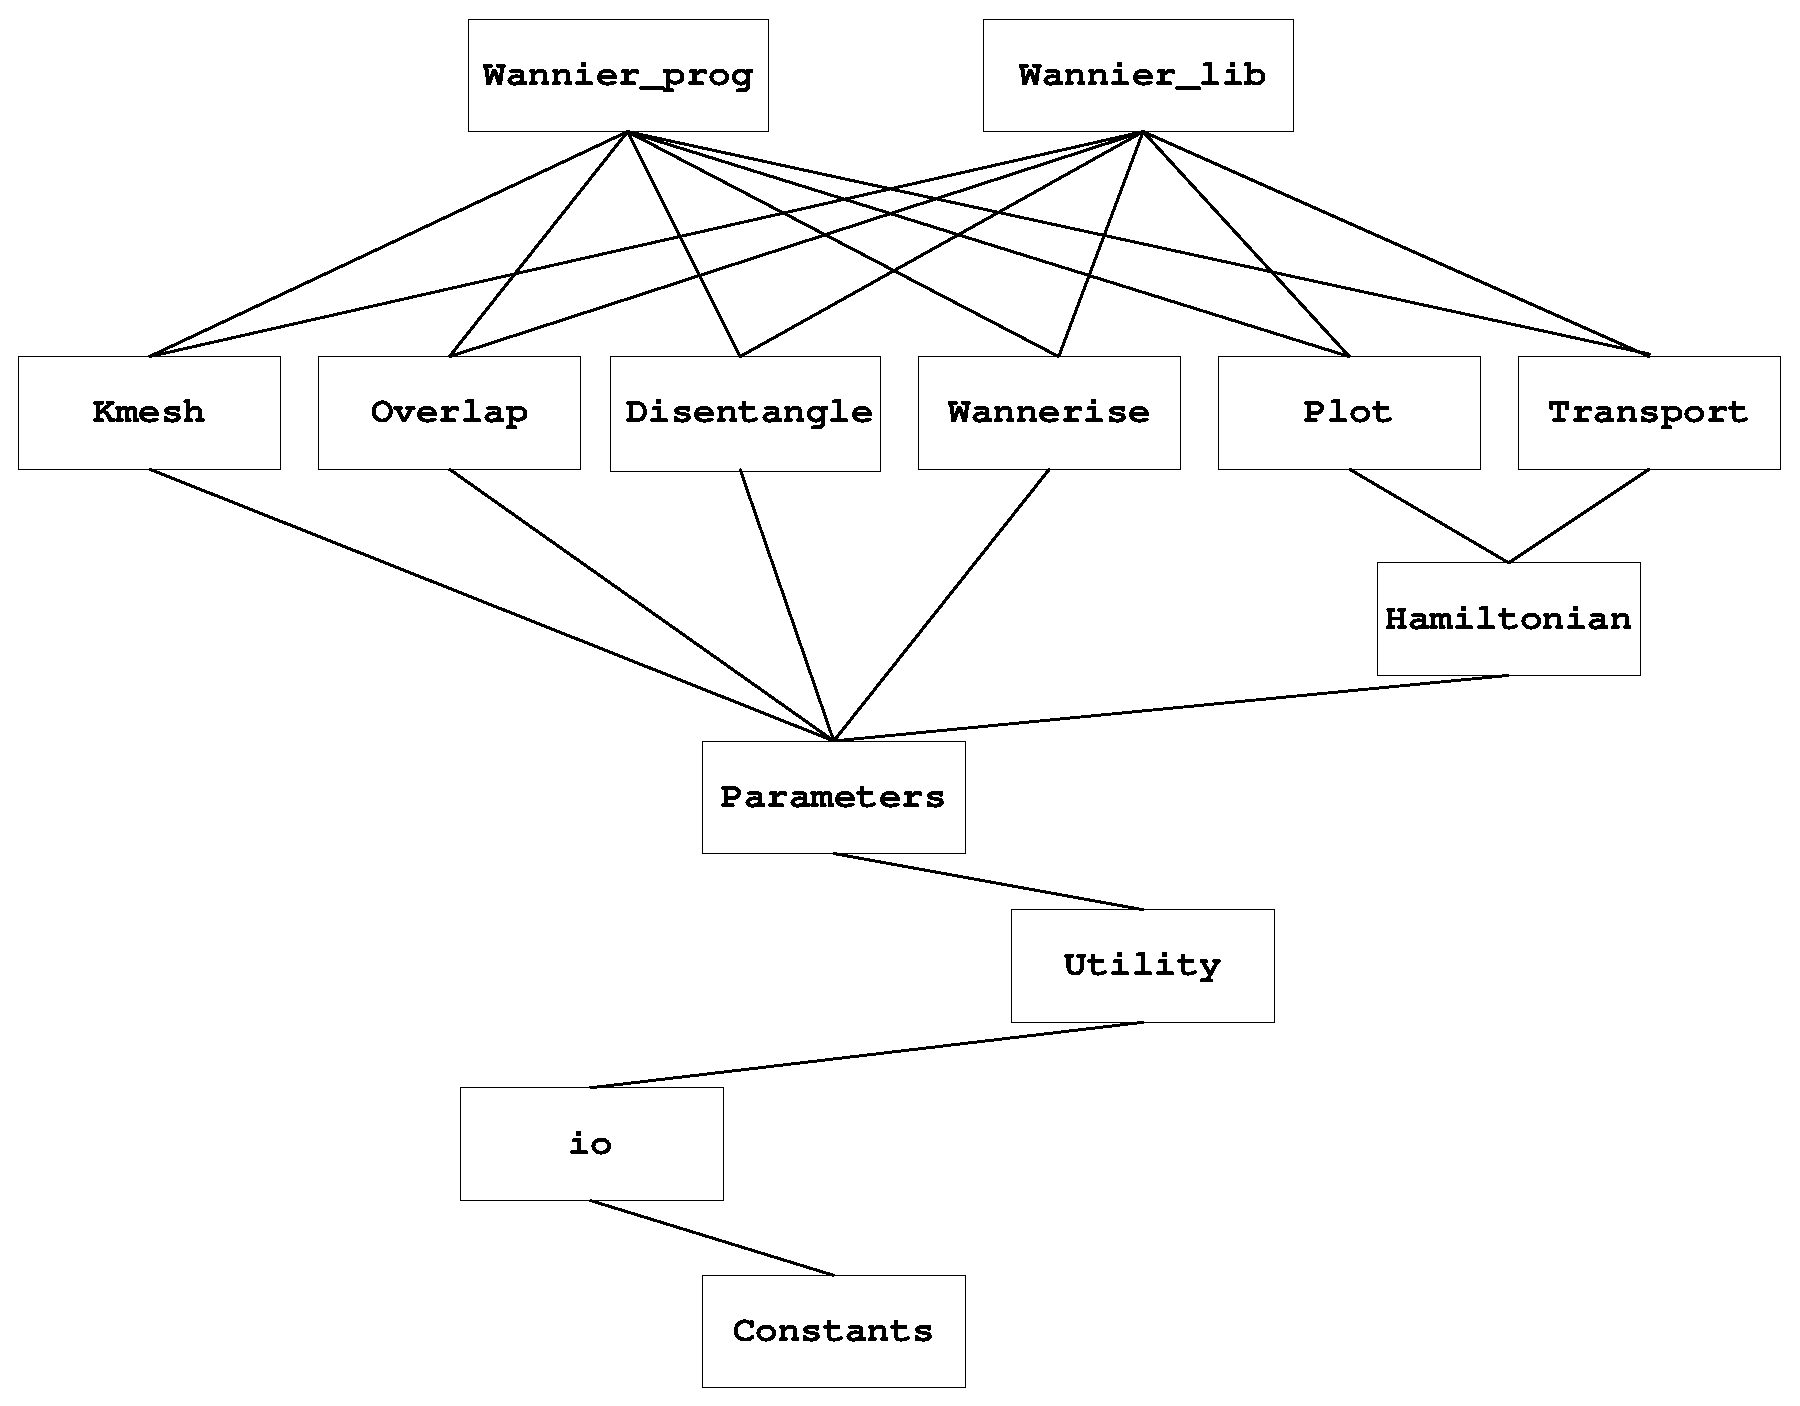
\includegraphics[width=5in]{overview.eps}
\caption{Schematic overview of the module structure of
  \wannier. Modules may only use data and subroutines from lower
  modules.}
\label{structure}
\end{center}
\end{figure}


\chapter{Wannier as a post-processing tool} \label{ch:wann-pp}

This is a description of how to use Wannier90 code as a
post-processing tool. 

The code must be run twice. On the first pass either the logical keyword
\verb#postproc_setup# must be set to \verb#.true.# in the input file
\verb#seedname.win# or the code must be run with the command line
option \verb#-pp#.  Running the code then generates the file
\verb#seedname.nnkp# which provides the information required to 
construct the $M_{mn}^{(\mathbf{k,b})}$ overlaps (MV Eq.~(25)) and
$A_{mn}^{(\mathbf{k})}$ (MV Eq.~(62), SMV Eq.~(22)). 

Once the overlaps and projection have been computed and written to
files \verb#seedname.mmn# and \verb#seedname.amn#, respectively,
set \verb#postproc_setup# to \verb#.false.# and run the code. Output is
written to the file \verb#seedname.wout#.


\section{nnkp file}

OUTPUT, if $\verb#postproc_setup#=\verb#.true.#$

The file \verb#seedname.nnkp# provides the information needed to
determine the required overlap elements $M_{mn}^{(\mathbf{k,b})}$ and
projections $A_{mn}^{(\mathbf{k})}$. It is written automatically when
the code is invoked with the \verb#-pp# command-line option (or when
\verb#postproc_setup=.true.# in \verb#seedname.win#. There should be
no need for the user to edit this file.

Much of the information in \verb#seedname.nnkp# is arranged in blocks
delimited by the strings \verb#begin block_name# \ldots
\verb#end block_name#, as described below. 


\subsection{Keywords}
The first line of the file is a user comment, e.g., the date and time:

\verb#File written on 12Feb2006 at 15:13:12#

\noindent 
The only logical keyword is \verb#calc_only_A#, eg,

\verb#calc_only_A  :  F#

\subsection{Real\_lattice block}
\begin{verbatim}
begin real_lattice
 2.250000   0.000000   0.000000
 0.000000   2.250000   0.000000
 0.000000   0.000000   2.250000
end real_lattice
\end{verbatim}

The real lattice vectors in units of Angstrom.


\subsection{Recip\_lattice block}
\begin{verbatim}
begin recip_lattice
 2.792527   0.000000   0.000000
 0.000000   2.792527   0.000000
 0.000000   0.000000   2.792527
end recip_lattice
\end{verbatim}

The reciprocal lattice vectors in units of inverse Angstrom.


\subsection{Kpoints block}
\begin{verbatim}
begin kpoints
  8
  0.00000   0.00000   0.00000
  0.00000   0.50000   0.00000
  .
  .
  .
  0.50000   0.50000   0.50000
end kpoints
\end{verbatim}

The first line in the block is the total number of k-points
\verb#num_kpts#. The subsequent \verb#num_kpts# lines specify the
k-points in crystallographic co-ordinates relative to the reciprocal
lattice vectors.


\subsection{Projections block}
\begin{verbatim}
begin projections
   n_proj
   centre   l  mr  r   
     z-axis   x-axis   zona   box-size   
   centre   l  mr  r   
     z-axis   x-axis   zona   box-size   
   .
   .
end projections
\end{verbatim}

\noindent
Notes:

\verb#n_proj#: integer; the number of projection centres, equal to the
number of Wannier functions \verb#num_wann#.

\verb#centre#: three real numbers; projection function centre
in crystallographic co-ordinates relative to the direct lattice
vectors.

\verb#l  mr  r#: three integers; $l$ and $m_\mathrm{r}$ specify the
angular part $\Theta_{lm_{\mathrm{r}}}(\theta,\varphi)$, and
$\mathrm{r}$ specifies the radial part $R_{\mathrm{r}}(r)$ of the
projection function (see Tables~\ref{tab:angular}, \ref{tab:hybrids}
and \ref{tab:radial}). 

\verb#z-axis#: three real numbers; default is
\verb#0.0 0.0 1.0#; defines the axis from which the polar angle
$\theta$ in spherical polar coordinates is measured.

\verb#x-axis#: three real numbers; must be orthogonal to
\verb#z-axis#; default is \verb#1.0 0.0 0.0# or a vector
perpendicular to \verb#z-axis# if \verb#z-axis# is given; defines the
axis from with the azimuthal angle $\varphi$ in spherical polar
coordinates is measured.

\verb#zona#: real number; the value of $\frac{Z}{a}$ associated
with the radial part of the atomic orbital. Units are in reciprocal
Angstrom.

\verb#box-size#: real number; the linear dimension of the real-space
box (or sphere) for calculating the overlap
$\langle\psi_{m\mathbf{k}}|\phi_{n}\rangle$ of a wavefunction with the
localised projection function. Units are in Angstrom. This feature is not
currently used.



\subsection{nnkpts block}
\begin{verbatim}
begin nnkpts
  10
  1   2   0  0  0
  .
  .
end nnkpts
\end{verbatim}

First line: \verb#nntot#, the number of nearest neighbours belonging
to each k-point of the Monkhorst-Pack mesh

Subsequent lines: \verb#nntot#$\times$\verb#num_kpts#
lines, ie, \verb#nntot# lines of data for each k-point of the mesh. 

Each line of consists of 5 integers. The first is the
k-point number \verb#nkp#. The second to the fifth specify it's nearest
neighbours $\mathbf{k+b}$: the second integer points to the k-point
that is the periodic image of the $\mathbf{k+b}$ that we want; the
last three integers give the G-vector, in reciprocal lattice units,
that brings the k-point specified by the second integer (which is in
the first BZ) to the actual $\mathbf{k+b}$ that we need.


\subsection{exclude\_bands block}
\begin{verbatim}
begin exclude_bands 
  8 
  1 
  2 
  .
  .
end exclude_bands
\end{verbatim}
To exclude bands (independent of k-point) from the calculation of the 
overlap and projection matricies, for example to ignore shallow-core states.
The first line is the number of states to exclude, the following lines give
the states for be excluded.


\subsection{An example of projections}\label{sec:proj_example}

As a concrete example: one wishes to have a set of four sp$^3$ projection
orbitals on, say, a carbon atom at (0.5,0.5,0.5) in fractional
co-ordinates relative to the direct lattice vectors. In this case
\verb#seedname.win# will contain the following lines:

\begin{verbatim}
begin projections
 C:l=-1
end projections
\end{verbatim}

and \verb#seedname.nnkp#, generated on the first pass of
\verb#wannier90# (with \verb#postproc_setup=T#), will contain: 

\begin{verbatim}
begin projections
   4
   0.50000    0.50000    0.50000    -1  1  1
     0.000  0.000  1.000   1.000  0.000  0.000   2.00  2.00
   0.50000    0.50000    0.50000    -1  2  1
     0.000  0.000  1.000   1.000  0.000  0.000   2.00  2.00
   0.50000    0.50000    0.50000    -1  3  1
     0.000  0.000  1.000   1.000  0.000  0.000   2.00  2.00
   0.50000    0.50000    0.50000    -1  4  1
     0.000  0.000  1.000   1.000  0.000  0.000   2.00  2.00
end projections
\end{verbatim}

where the first line tells us that in total four projections are
specified, and the subsquent lines provide the projection centre, the
angular and radial parts of the orbital (see
Section~\ref{sec:orbital-defs} for definitions), the $z$ and $x$ axes,
and the diffusivity and cut-off radius for the projection orbital.

\textsc{pwscf}, or any other \textit{ab initio} electronic structure
code, then reads \verb#seedname.nnkp# file, calculates the projections
and writes them to \verb#seedname.amn#. 




%\subsection{Things to add}
%
%\begin{itemize}
%\item List of states to exclude from the calculation
%  (\verb#exclude_bands#)
%\end{itemize}
%
%Notes:
%
%It would be desirable to be able to control which bands to include. One
%might perform a `nscf' calculation for 16 bands and want to
%\begin{enumerate}
%\item ignore the lowest $n$ bands (e.g., only look at conduction states)
%\item take the lowest $n$ bands (e.g., only look at valence states)
%\item ignore an isolated set of bands in the middle of the energy
% range (e.g., the d orbitals in ZnTe)
%\end{enumerate}
%As calculating overlaps and projections is time consuming we want to
%cut out these states at the \verb#pw2wannier90# stage, not in
%\verb#wannier90#. 
%We can probably specify all this in \verb#seedname.win# and pass
%an explicit list of states to include (or exclude) in
%\verb#seedname.nnkp#.
%

\section{Mmn file} 

INPUT. 

The file \verb#seedname.mmn# contains the overlaps
$M_{mn}^{(\mathbf{k,b})}$.

First line: a user comment, e.g., the date and time

Second line: 3 integers: \verb#num_bands#, \verb#num_kpts#,
\verb#nntot#

Then: $\verb#num_kpts#\times\verb#nntot#$ blocks of data:
 
First line of each block: 5 integers. The first specifies the
$\mathbf{k}$ (i.e., gives the ordinal corresponding to its position in
the list  of k-points in \verb#seedname.win#). The 2nd to 5th integers
specify $\mathbf{k+b}$. The  2nd integer, in particular, points to the
k-point on the list that is a  periodic image of $\mathbf{k+b}$, and
in particular is the image that is actually mentioned in the list. The 
last three integers specify the $\mathbf{G}$ vector, in  reciprocal
lattice units, that brings the k-point specified by the fourth
integer, and that thus lives inside the first BZ zone, to the actual
$\mathbf{k+b}$ that we need.

Subsequent $\verb#num_bands#\times\verb#num_bands#$ lines of each
block: two real numbers per line. These are the real and imaginary
parts, respectively, of the actual scalar product
$M_{mn}^{(\mathbf{k,b})}$ for $m,n \in [1,\verb#num_bands#]$. The
order of these elements is such that the first index $m$ is fastest.


\section{Amn file}

INPUT.

The file \verb#seedname.amn# contains the projection
$A_{mn}^{(\mathbf{k})}$.

First line: a user comment, e.g., the date and time

%Second line: a single integer, either 0 or 1. See below for explanation.

Second line: 3 integers: \verb#num_bands#, \verb#num_kpts#, \verb#num_wann#

                                     
Subsequently
$\verb#num_bands#\times\verb#num_wann#\times\verb#num_kpts#$ 
lines: 3 integers and 2 real numbers on each line. The first 
two integers are the band indices $m$ and $n$. The third integer specifies
the $\mathbf{k}$ by giving the ordinal corresponding to its position
in the list of $k$-points in \verb#seedname.win#. The real numbers
are the real and imaginary parts, respectively, of the actual
$A_{mn}^{(\mathbf{k})}$.

%The flag in the second line of \verb#seedname.amn# is present in order
%to give the \textit{ab initio} code some freedom to choose the shape
%of the projections itself. There are two possibilities:
%\begin{itemize}
%\item If it is 0, then
%\verb#wannier90# assumes that the projections in \verb#seedname.amn#
%have been calculated as specified in \verb#seedname.nnkp# and proceeds
%(if hybrid orbitals are required) to mix them in the correct manner to
%obtain projections onto the desired orbitals specified in
%\verb#seedname.win#
%\item If it is 1, then \verb#wannier90# ignores the specification of
%  the projection orbital shapes in \verb#seedname.win# and takes the
%  \verb#seedname.amn# file `as is', i.e., does no mixing.
%\end{itemize}

%In terms of the example of Section~\ref{sec:proj_example}, let us
%suppose that this flag is set to 0. Then 
%\verb#seedname.amn# contains the overlaps of a wavefunction
%$\psi_{m\mathbf{k}}$ with an atomic s and three p-orbitals
%$\{\verb#s#,\verb#px#,\verb#py#,\verb#pz#\}$.
%\verb#wannier90# will read 
%\verb#seedname.amn# and calculate the projection
%$A_{mn}^{(\mathbf{k})}$ of a $\psi_{m\mathbf{k}}$ onto
%four sp$^3$ orbitals  $\{\phi_{n}\}$ (specified in \verb#seedname.win# by
%\verb#l=-1#, or the string \verb#sp3#)
%by linear mixing as follows:  

%\begin{eqnarray}
%A_{mn}^{(\mathbf{k})} & = & \langle\psi_{m\mathbf{k}}|\phi_{n}\rangle
%                      \nonumber \\
%                      & = &
%                      \langle\psi_{m\mathbf{k}}|\verb#sp3-n#\rangle
%                      \nonumber \\ 
%                      & = &
% \frac{1}{2}\left[\langle\psi_{m\mathbf{k}}|\verb#s#\rangle \pm
% \langle\psi_{m\mathbf{k}}|\verb#px#\rangle \pm
% \langle\psi_{m\mathbf{k}}|\verb#py#\rangle \pm
% \langle\psi_{m\mathbf{k}}|\verb#pz#\rangle\right], \label{eq:Amn}
%\end{eqnarray} 
%
%where the matrix elements on the right-hand side are taken from
%\verb#seedname.amn#. Projections corresponding to four sp$^{3}$
%orbitals \verb#sp3-1#, \verb#sp3-2#, \verb#sp3-3#, and \verb#sp3-4# --
%see Section~\ref{sec:orbital-defs} -- are
%obtained with appropriate choice of the signs in Eq.~(\ref{eq:Amn}): 
%($+$,$+$,$+$), ($+$,$-$,$-$), ($-$,$+$,$-$) and
%($-$,$-$,$+$).


\section{eig file}

INPUT. 

Required if any of \verb#disentanglement#, \verb#plot_bands#,
   \verb#plot_fermi_surface# or \verb#plot_dos# are \verb#.true.#

The file \verb#seedname.eig# contains the Kohn-Sham eigenvalues
     $\varepsilon_{n\mathbf{k}}$ (in eV) at each point in the
     Monkhorst-Pack mesh.

Each line consist of two integers and a real number. The first integer
is the band index, the second integer gives the ordinal corresponding
to the $k$-point in the list of $k$-points in \verb#seedname.win#,
and the real number is the eigenvalue. 

E.g.,

\begin{verbatim}
           1           1  -6.43858831271328
           2           1   19.3977795287297
           3           1   19.3977795287297
           4           1   19.3977795287298
\end{verbatim}


\section{Interface with PWSCF}

\begin{enumerate}
\item Run `scf'/'nscf' calculation(s) with \verb#pw#
\item Run \verb#wannier90# with \verb#postproc_setup#~=~\verb#.true.# to
  generate \verb#seedname.nnkp#
\item Run \verb#pw2wannier90#. First it reads \verb#pw2wannier90.in#,
  which defines \verb#prefix# and \verb#outdir# for the underlying `scf'
  calculation, as well as the name of the file \verb#seedname.nnkp#,
  and does a consistency check between the direct and reciprocal lattice
  vectors read from \verb#seedname.nnkp# and those defined in the
  files specified by \verb#prefix#. \verb#pw2wannier90# generates
  \verb#seedname.mmn#, \verb#seedname.amn# and \verb#seedname.eig#
\item Run \verb#wannier90# with \verb#postproc_setup#~=~\verb#.false.# to
  disentangle bands (if required) and localise Wannier functions.
\end{enumerate}

\subsection{pw2wannier90.in}

A number of keywords may be specified in the \verb#pw2wannier90# input file:

   \verb#outdir# -- Location to write output files. Default is \verb#`./'#

   \verb#prefix# -- Prefix for the PWscf calculation. Default is \verb#` '#

   \verb#seedname# -- Seedname for the Wannier90 calculation. Default
   is \verb#`wannier'#

   \verb#spin_component# -- Spin component. Takes values \verb#`up'#,

   \verb#`down'# or \verb#`none'# (default).

%   wan_mode = 'standalone'

   \verb#write_unk# -- Set to \verb#true# to write the periodic part
   of the Bloch functions for plotting in Wannier90. Default is
   \verb#.false.#

   \verb#wvfn_formatted# -- Set to \verb#.true.# to write formatted
   wavefunctions. Default is \verb#.false.# (only relevant if
   \verb#write_unk=.true.#)

   \verb#write_amn# -- Set to \verb#.false.# if
   $A_{mn}^{(\mathbf{k})}$ not required. Default is \verb#.true.#

   \verb#write_mmn# -- Set to \verb#.false.# if
   $M_{mn}^{(\mathbf{k,b})}$ not required. Default is \verb#.true.#


\chapter{\wannier\ as a library}\label{ch:wann-lib}

This is a description of the interface between any external program
and the wannier code. There are two subroutines: \verb#wannier_setup#
and \verb#wannier_run#. Calling \verb#wannier_setup# will return
information required to construct the $M_{mn}^{(\mathbf{k,b})}$
overlaps (Ref.~\cite{marzari-prb97}, Eq.~(25)) and
$A_{mn}^{(\mathbf{k})}=\left\langle
  \psi_{m\mathbf{k}}|g_{n}\right\rangle$ projections
(Ref.~\cite{marzari-prb97}, Eq.~(62); Ref.~\cite{souza-prb01},
Eq.~(22)). Once the overlaps and projection have been computed,
calling \verb#wannier_run# activates the minimisation and plotting
routines in \wannier.

%\section{Dependencies}
%\begin{itemize}
%\item Parameters
%\item IO
%\item Kmesh
%\item Overlap
%\item Wannierise
%\end{itemize}

\section{Subroutines}

\subsection{{\tt wannier\_setup}}

{\noindent \bf \verb#wannier_setup(seed_name,mp_grid,num_kpts,real_lattice,recip_lattice,#\\
\verb#              kpt_latt,num_bands_tot,num_atoms,atom_symbols,atoms_cart,#\\
\verb#              gamma_only,spinors,nntot,nnlist,nncell,num_bands,num_wann,proj_site,#\\
\verb#              proj_l,proj_m,proj_radial,proj_z,proj_x,proj_zona,#\\
\verb#              exclude_bands)#}

\begin{itemize}
\item \verb#character(len=*), intent(in) :: seed_name#\\ The seedname
  of the current calculation.
\item \verb#integer, dimension(3), intent(in) :: mp_grid#\\ The
  dimensions of the {Monkhorst-Pack} k-point grid.
\item \verb#integer, intent(in) :: num_kpts#\\ The number of k-points on
  the {Monkhorst-Pack} grid.
\item \verb#real(kind=dp), dimension(3,3), intent(in) :: real_lattice#\\
  The lattice vectors in Cartesian co-ordinates in units of Angstrom.
\item \verb#real(kind=dp), dimension(3,3), intent(in) :: recip_lattice#\\
  The reciprocal lattice vectors in Cartesian co-ordinates in units of reciprocal Angstrom.
\item
  \verb#real(kind=dp), dimension(3,num_kpts), intent(in) :: kpt_latt#\\
  The positions of the k-points in fractional co-ordinates
  relative to the reciprocal lattice vectors.
\item \verb#integer, intent(in) :: num_bands_tot#\\ The total number of bands in the
first-principles calculation (note: including semi-core states).
\item \verb#integer, intent(in) :: num_atoms#\\ The total number of atoms
  in the system.
\item \verb#character(len=20), dimension(num_atoms),#
      \verb# intent(in) :: atom_symbols#\\ The elemental symbols of
      the atoms.
\item \verb#real(kind=dp), dimension(3,num_atoms),#
      \verb#intent(in) :: atoms_cart#\\ The positions of the atoms in
      Cartesian co-ordinates in Angstrom.
\item \verb#logical, intent(in) :: gamma_only#\\ Set to \texttt{.true.} if the
  underlying electronic structure calculation has been performed with
  only $\Gamma$-point sampling and, hence, if the Bloch eigenstates
  that are used to construct $A_{mn}^{(\mathbf{k})}$ and
  $M_{mn}^{\mathbf{(k,b)}}$ are real.
\item \verb#logical, intent(in) :: spinors#\\ Set to \texttt{.true.} if
  underlying electronic structure calculation has been performed with
  spinor wavefunctions. Note: the only effect this has is that wannier90
  will expect half the usual number of projections.
\item \verb#integer, intent(out) :: nntot#\\ The
  total number of nearest neighbours for each k-point. 
\item \verb#integer, dimension(num_kpts,num_nnmax),#
      \verb# intent(out) :: nnlist#\\
      The list of nearest neighbours for each k-point.
\item \verb#integer,dimension(3,num_kpts,num_nnmax),#
      \verb# intent(out) :: nncell#\\ 
      The vector, in fractional reciprocal lattice co-ordinates, that
      brings the \verb#nn#$^{\mathrm{th}}$ nearest neighbour of
      k-point \verb#nkp# to its periodic image that
      is needed for computing the overlap 
      $M_{mn}^{(\mathbf{k,b})}$.
\item \verb#integer, intent(out) :: num_bands#\\ The number of bands in the
first-principles calculation used to form the overlap matricies (note: excluding eg. semi-core states).
\item \verb#integer, intent(out) :: num_wann#\\ The number of MLWF
  to be extracted.
\item  \verb#real(kind=dp), dimension(3,num_bands_tot), intent(out) :: proj_site# \\
Projection function centre
in crystallographic co-ordinates relative to the direct lattice
vectors.
\item \verb#integer, dimension(num_bands_tot), intent(out) :: proj_l#\\
 $l$  specifies the angular part $\Theta_{lm_{\mathrm{r}}}(\theta,\varphi)$ of the
projection function  (see Tables~\ref{tab:angular}, \ref{tab:hybrids}
and \ref{tab:radial}). 
\item \verb#integer, dimension(num_bands_tot), intent(out) :: proj_m#\\
 $m_\mathrm{r}$ specifies the angular part $\Theta_{lm_{\mathrm{r}}}(\theta,\varphi)$, of the
projection function
 (see Tables~\ref{tab:angular}, \ref{tab:hybrids}
and \ref{tab:radial}). 
\item \verb#integer, dimension(num_bands_tot), intent(out) :: proj_radial#\\
$\mathrm{r}$ specifies the radial part $R_{\mathrm{r}}(r)$ of the
projection function 
(see Tables~\ref{tab:angular}, \ref{tab:hybrids}
and \ref{tab:radial}). 
\item  \verb#real(kind=dp), dimension(3,num_bands_tot), intent(out) :: proj_z#\\
Defines the axis from which the polar angle
$\theta$ in spherical polar coordinates is measured. Default is
\verb#0.0 0.0 1.0#.
\item  \verb#real(kind=dp), dimension(3,num_bands_tot), intent(out) :: proj_x#\\
Must be orthogonal to
\verb#z-axis#; default is \verb#1.0 0.0 0.0# or a vector
perpendicular to \verb#proj_z# if \verb#proj_z# is given; defines the
axis from with the azimuthal angle $\varphi$ in spherical polar
coordinates is measured.
\item \verb#real(kind=dp), dimension(num_bands_tot), intent(out) :: proj_zona#\\
The value of $\frac{Z}{a}$ associated
with the radial part of the atomic orbital. Units are in reciprocal
Angstrom.
\item \verb#integer, dimension(num_bands_tot), intent(out) :: exclude_bands#\\ 
      Kpoints independant list of bands to exclude from the
      calculation of the MLWF (e.g., semi-core states). 

\end{itemize}

Conditions:
\begin{itemize}
\cond $\verb#num_kpts# = \verb#mp_grid(1)# \times \verb#mp_grid(2)#
\times \verb#mp_grid(3)#$.
\cond $\verb#num_nnmax# = 12$
\end{itemize}

This subroutine returns the information required to determine the
required overlap elements $M_{mn}^{(\mathbf{k,b})}$ and
projections $A_{mn}^{(\mathbf{k})}$,
i.e., \verb#M_matrix# and \verb#A_matrix#, described in
Section~\ref{wannier_run}. 

For the avoidance of doubt, \verb#real_lattice(1,2)# is the
$y-$component of the first lattice vector $\mathbf{A}_{1}$, etc.

The list of nearest neighbours of a particular k-point \verb#nkp# is
given by \verb#nnlist(nkp,1:nntot)#.

Additionally, the parameter \verb#shell_list#
may be specified in the \wannier\ input file.

\subsection{{\tt wannier\_run}} \label{wannier_run}

{\noindent \bf \verb#wannier_run(seed_name,mp_grid,num_kpts,real_lattice,recip_lattice,#\\
\verb#            kpt_latt,num_bands,num_wann,nntot,num_atoms,atom_symbols,#\\
\verb#            atoms_cart,gamma_only,M_matrix_orig,A_matrix,eigenvalues,#\\
\verb#            U_matrix,U_matrix_opt,lwindow,wann_centres,wann_spreads,#\\
\verb#            spread#)}

\begin{itemize}
\item \verb#character(len=*), intent(in) :: seed_name#\\ The seedname
  of the current calculation.
\item \verb#integer, dimension(3), intent(in) :: mp_grid#\\ The
  dimensions of the {Monkhorst-Pack} k-point grid.
\item \verb#integer, intent(in) :: num_kpts#\\ The number of k-points on
  the {Monkhorst-Pack} grid.
\item \verb#real(kind=dp), dimension(3,3),#
      \verb# intent(in) :: real_lattice#\\ The lattice vectors in
      Cartesian co-ordinates in units of Angstrom. 
\item \verb#real(kind=dp), dimension(3,3), intent(in) :: recip_lattice#\\
  The reciprical lattice vectors in Cartesian co-ordinates in units of inverse Angstrom.
\item \verb#real(kind=dp), dimension(3,num_kpts),#
      \verb# intent(in) :: kpt_latt#\\ The positions of the k-points in
      fractional co-ordinates relative to the reciprocal lattice
      vectors.
\item \verb#integer, intent(in) :: num_bands#\\ The total number of
      bands to be processed.
\item \verb#integer, intent(in) :: num_wann#\\ The number of MLWF to
  be extracted. 
\item \verb#integer, intent(in) :: nntot#\\ The number of
  nearest neighbours for each k-point.
\item \verb#integer, intent(in) :: num_atoms#\\ The total number of atoms
  in the system.
\item \verb#character(len=20), dimension(num_atoms),#
      \verb# intent(in) :: atom_symbols#\\ The elemental symbols of
      the atoms.
\item \verb#real(kind=dp), dimension(3,num_atoms),#
      \verb#intent(in) :: atoms_cart#\\ The positions of the atoms in
      Cartesian co-ordinates in Angstrom.
\item \verb#logical, intent(in) :: gamma_only#\\ Set to \texttt{.true.} if the
  underlying electronic structure calculation has been performed with
  only $\Gamma$-point sampling and, hence, if the Bloch eigenstates
  that are used to construct $A_{mn}^{(\mathbf{k})}$ and
  $M_{mn}^{\mathbf{(k,b)}}$ are real.
\item \verb#complex(kind=dp),#
      \verb# dimension(num_bands,num_bands,nntot,num_kpts),#\\
      \verb#                  intent(in) :: M_matrix#\\ 
      The matrices of overlaps between neighbouring periodic parts of
      the Bloch eigenstates at each k-point, $M_{mn}^{(\mathbf{(k,b)})}$
      (Ref.~\cite{marzari-prb97}, Eq.~(25)).
\item \verb#complex(kind=dp), dimension(num_bands,num_wann,num_kpts),#\\
      \verb#                  intent(in) :: A_matrix# \\The matrices
      describing the projection of \verb#num_wann# trial orbitals on
      \verb#num_bands# Bloch states at each k-point,
      $A_{mn}^{(\mathbf{k})}$ (Ref.~\cite{marzari-prb97}, Eq.~(62);
      Ref.~\cite{souza-prb01}, Eq.~(22)).
\item \verb#real(kind=dp), dimension(num_bands,num_kpts),#
      \verb#intent(in) :: eigenvalues#\\ The
      eigenvalues $\varepsilon_{n\mathbf{k}}$ corresponding to the
      eigenstates, in eV.
\item \verb#complex(kind=dp), dimension(num_wann,num_wann,num_kpts),#\\
      \verb#                  intent(out) :: U_matrix#\\ The unitary
      matrices at each k-point (Ref.~\cite{marzari-prb97}, Eq.~(59))
\item \verb#complex(kind=dp), dimension(num_bands,num_wann,num_kpts),#\\
      \verb#                   intent(out) :: U_matrix_opt#\\ The
      unitary matrices that describe the optimal sub-space at each
      k-point (see Ref.~\cite{souza-prb01}, Section~{\sc IIIa}). The array is
      packed (see below) 
\item \verb#logical, dimension(num_bands,num_kpts), intent(out) :: lwindow#\\ 
       The element \verb#lwindow(nband,nkpt)# is {\tt .true.} if the band
{\tt nband} lies within the outer energy window at kpoint {\tt nkpt}.
\item \verb#real(kind=dp), dimension(3,num_wann), intent(out) :: wann_centres#\\   
      The centres of the MLWF in Cartesian co-ordinates in Angstrom. 
\item \verb#real(kind=dp), dimension(num_wann), intent(out) :: wann_spreads#\\ 
      The spread of each MLWF in \AA$^{2}$.
\item \verb#real(kind=dp), dimension(3), intent(out) ::#
      \verb#spread#\\ 
      The values of $\Omega$, $\Omega_{\mathrm{I}}$ and
      $\tilde{\Omega}$ (Ref.~\cite{marzari-prb97}, Eq.~(13)). 
\end{itemize}

Conditions:
\begin{itemize}
\cond $\verb#num_wann# \le \verb#num_bands#$
\cond $\verb#num_kpts# = \verb#mp_grid(1)# \times \verb#mp_grid(2)#
\times \verb#mp_grid(3)#$.
\end{itemize}

If $\verb#num_bands# = \verb#num_wann#$ then \verb#U_matrix_opt# is the identity matrix and
\verb#lwindow=.true.#

For the avoidance of doubt, \verb#real_lattice(1,2)# is the
$y-$component of the first lattice 
vector $\mathbf{A}_{1}$, etc.

\begin{eqnarray*}
\verb#M_matrix(m,n,nn,nkp)# & = & \left\langle u_{m\mathbf{k}} |
u_{n\mathbf{k+b}}\right\rangle\\
\verb#A_matrix(m,n,nkp)# & = &
\left\langle \psi_{m\mathbf{k}}|g_{n}\right\rangle\\
\verb#eigenvalues(n,nkp)# &=& \varepsilon_{n\mathbf{k}}
\end{eqnarray*}
where
\begin{eqnarray*}
\mathbf{k} &=&\verb#kpt_latt(1:3,nkp)#\\
\mathbf{k+b}&=& \verb#kpt_latt(1:3,nnlist(nkp,nn))# +
\verb#nncell(1:3,nkp,nn)# 
\end{eqnarray*}
and
$\left\{|g_{n}\rangle\right\}$ are a set of initial trial
orbitals. These are
typically atom or bond-centred Gaussians that are modulated by
appropriate spherical harmonics. 

Additional parameters should be specified in the \wannier\ input
file.



\chapter{Transport Calculations with \wannier\ }\label{ch:transport}

By setting $\verb#transport#=\verb#TRUE#$, \wannier\ will calculate
the quantum conductance and density of states of a one-dimensional
system. The results will be written to files \verb#seedname_qc.dat#
and \verb#seedname_dos.dat#, respectively.

The system for which transport properties are calculated is determined
by the keyword \verb#transport_mode#.

\section{\tt transport\_mode = bulk}

Quantum conductance and density of states are calculated for a perfectly
periodic one-dimensional conductor. If $\verb#tran_read_ht#=\verb#FALSE#$
the transport properties are calculated using the Hamiltonian in the Wannier 
function basis of the system found by \wannier. Setting 
$\verb#tran_read_ht#=\verb#TRUE#$ allows the user to provide an 
external Hamiltonian matrix file {\tt seedname\_htB.dat}, from which
the properties are found. See Section~\ref{sec:post-p} for more details of 
the keywords required for such calculations.

\section{\tt transport\_mode = lcr}

Quantum conductance and density of states are calculated 
for a system where semi-infinite, left and right leads
are connected through a central conductor region. This is known 
as the \emph{lcr} system.
Details of the method is described in Ref. \cite{Nardelli}.

In \wannier\ two options exist for performing such calculations: 
\begin{itemize}
\item If $\verb#tran_read_ht#=\verb#TRUE#$ the external Hamiltonian 
files {\tt seedname\_htL.dat, seedname\_htLC.dat, seedname\_htC.dat, 
seedname\_htCR.dat, seedname\_htR.dat} are read and used to compute 
the transport properties. 
\item If $\verb#tran_read_ht#=\verb#FALSE#$, then the transport
calculation is performed automatically using the Wannier functions as a
basis and the 2c2 geometry described in Section~\ref{sec:2c2}.
\end{itemize}

\section{Automated lcr Transport Calculations: The 2c2 Geometry}
\label{sec:2c2}

Calculations using the 2c2 geometry provide a method to calculate the
transport properties of an lcr system from a single \wannier\ calculation.
The Hamiltonian matrices which the five external files provide in the 
$\verb#tran_read_ht#=\verb#TRUE#$ case are instead built from the 
Wannier function basis directly. As such, strict rules apply to the system geometry, 
which is shown in Figure~\ref{fig:2c2}. These rules are as follows:
\begin{itemize}
\item Left and right leads must be identical and periodic.
\item Supercell must contain two principal layers (PLs) of lead on the left,
a central conductor region and two principal layers of lead on the right.
\item The conductor region must contain enough lead such that the
disorder does not affect the principal layers of lead either side.
\item A single \textbf{k}-point (Gamma) must be used.
\end{itemize}

\begin{figure}[h]
\centering
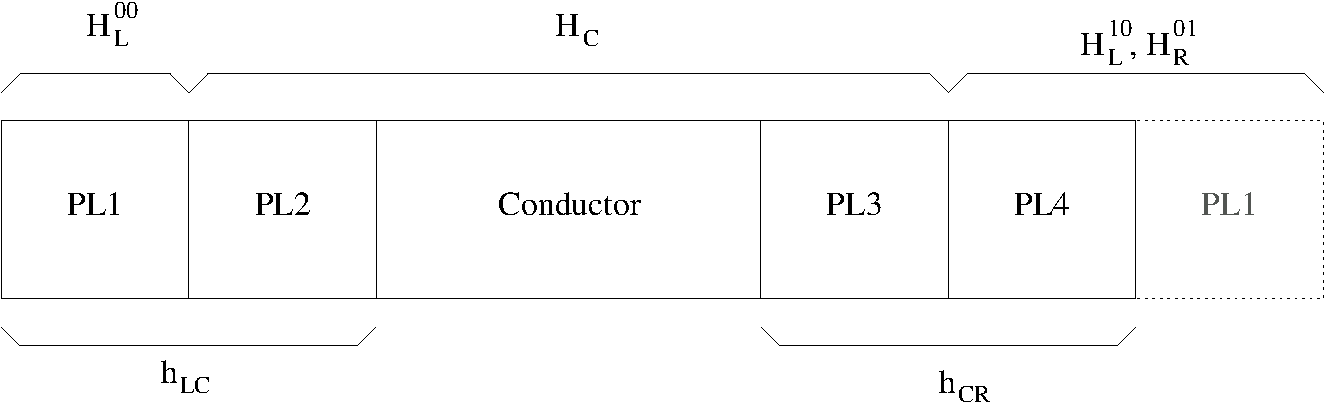
\includegraphics[height=4cm]{lcr_2c2}
\caption{Schematic illustration of the supercell required for 2c2
lcr calculations, showing where each of the Hamiltonian matrices
are derived from. Four principal layers (PLs) are required plus the
conductor region.}
\label{fig:2c2}
\end{figure}

In order to build the Hamiltonians, Wannier  functions are first 
sorted according to position and then type if a number of Wannier
functions exist with a similar centre (eg. \emph{d}-orbital type Wannier
functions centred on a Cu atom). Next, consistent parities of Wannier
function are enforced. To distingiush between different types of Wannier function
and assertain relative parities, a signature of each Wannier function 
is computed. The signature is formed of 20 integrals which have
different spatial dependence. They are given by:

\begin{equation}
I=\frac{1}{V}\int_V g(\mathbf{r})w(\mathbf{r})d\mathbf{r}
\label{eq:sig_ints}
\end{equation}

where $V$ is the volume of the cell, $w(\mathbf{r})$ is the Wannier 
function and $g(\mathbf{r})$ are the set of functions:

\begin{eqnarray}
g(\mathbf{r})=&\left\lbrace1,\sin\left(\frac{2\pi (x-x_c)}{L_x}\right),
											 \sin\left(\frac{2\pi (y-y_c)}{L_y}\right),
											 \sin\left(\frac{2\pi (z-z_c)}{L_z}\right),
											 \sin\left(\frac{2\pi (x-x_c)}{L_x}\right)
											 \sin\left(\frac{2\pi (y-y_c)}{L_y}\right),\right.\nonumber \\
										   &\left.\sin\left(\frac{2\pi (x-x_c)}{L_x}\right)
											 \sin\left(\frac{2\pi (z-z_c)}{L_z}\right),
											 ... \right\rbrace
\label{eq:g(r)}
\end{eqnarray}
upto third order in powers of sines. Here, the supercell has dimension 
$(L_x,L_y,L_z)$ and the Wannier function has centre $\mathbf{r}_c=(x_c,y_c,z_c)$.
Each of these integrals may be written as linear combinations 
of the following sums:

\begin{equation}
S_n(\mathbf{G})=\displaystyle{e^{i\mathbf{G.r}_{c}}\sum_{m}U_{mn}\tilde{u}_{m\Gamma}^{*}(\mathbf{G})}
\end{equation}

where $n$ and $m$ are the Wannier function and band indexes, 
$\mathbf{G}$ is a G-vector, $U_{mn}$ is the unitary matrix that 
transforms from the Bloch reopresentation of the system to the 
maximally-localised Wannier function basis and 
$\tilde{u}_{m\Gamma}^{*}(\mathbf{G})$ are the conjugates of the 
Fourier transforms of the periodic parts of the Bloch states at the $\Gamma\!$
-point. The complete set of $\tilde{u}_{m\mathbf{k}}(\mathbf{G})$ 
are often outputted by plane-wave DFT codes. However, to calculate the 20 
signature integrals, only 32 specific $\tilde{u}_{m\mathbf{k}}(\mathbf{G})$ 
are required. These are found in an addition file (\verb#seedname.unkg#) 
that should be provided by the interface between the DFT code and \wannier\ . 
A detailed description of this file may be found in Section~\ref{sec:files_unkg}.

Additionally, the following keywords are also required in the input file:
\begin{itemize}
\item \verb#tran_num_ll# : The number of Wannier functions in a 
principal layer.
\item \verb#tran_num_cell_ll# : The number of unit cells in one 
principal layer of lead
\end{itemize}

A further parameter related to these calculations is
\verb#tran_group_threshold#.

Examples of how 2c2 calculations are preformed can be found 
in the \wannier\ Tutorial. 


\chapter{Files}


\section{{\tt seedname.win}}
INPUT. The master input file; contains the specification of the system
and any parameters for the run. For a description of input parameters,
see Chapter~\ref{chap:parameters}; for examples, see
Section~\ref{winfile} and the \wannier\
Tutorial.

\subsection{Units}

The following are the dimensional quantities that are
specified in the master input file:

\begin{itemize}
\item Direct lattice vectors
\item Positions (of atomic or projection) centres in real space
\item Energy windows
\item Positions of k-points in reciprocal space
\item Convergence thresholds for the minimisation of $\Omega$
%%\item \verb#zona# and \verb#box-size# (see Section~\ref{sec:proj})
\item \verb#zona# (see Section~\ref{sec:proj})
\item \verb#wannier_plot_cube#: cut-off radius for plotting WF in
  Gaussian cube format
\end{itemize}

Notes:

\begin{itemize}
\item The units (either \verb#ang#
  (default) or \verb#bohr#) in which the lattice vectors, atomic
  positions or projection centres are given can be set in the first
  line of the blocks 
  \verb#unit_cell_cart#, \verb#atoms_cart# and \verb#projections#,
  respectively, in \verb#seedname.win#.
\item Energy is always in eV.
\item Convergence thresholds are always in \AA$^{2}$
\item Positions of k-points are always in crystallographic
  coordinates relative to the reciprocal lattice vectors.
%%\item \verb#box-size# and \verb#zona# always in Angstrom and
%%  reciprocal Angstrom, respectively
\item \verb#zona# is always in reciprocal Angstrom (\AA$^{-1}$)
\item The keyword \verb#length_unit# may be set to \verb#ang#
  (default) or \verb#bohr#, in order to set the units in which the
  quantities in the output file {\tt seedname.wout} are written.
\item \verb#wannier_plot_radius# is in Angstrom
\end{itemize}

The reciprocal lattice vectors
$\{\mathbf{B}_{1},\mathbf{B}_{2},\mathbf{B}_{3}\}$ are defined in
terms
of the direct lattice vectors
$\{\mathbf{A}_{1},\mathbf{A}_{2},\mathbf{A}_{3}\}$ by the equation

\begin{equation}
\mathbf{B}_{1} = \frac{2\pi}{\Omega}\mathbf{A}_{2}\times\mathbf{A}_{3}
\ \ \ \mathrm{etc.},
\end{equation}

where the cell volume is
$V=\mathbf{A}_{1}\cdot(\mathbf{A}_{2}\times\mathbf{A}_{3})$.

\section{{\tt seedname.mmn}}
INPUT. Written by the underlying electronic structure code. See
Chapter~\ref{ch:wann-pp} for details.

\section{{\tt seedname.amn}}
INPUT. Written by the underlying electronic structure code. See
Chapter~\ref{ch:wann-pp} for details. 

\section{{\tt seedname.eig}}
INPUT. Written by the underlying electronic structure code. See
Chapter~\ref{ch:wann-pp} for details.

\section{{\tt seedname.nnkp}} \label{sec:old-nnkp}
OUTPUT. Written by \wannier\ when {\tt postproc\_setup=.TRUE.} (or,
alternatively, when \wannier\ is run with the {\tt -pp} command-line
option). See Chapter~\ref{ch:wann-pp} for details.

\section{{\tt seedname.wout}}
OUTPUT. The master output file. Here we give a description of the main
features of the output. The verbosity of the output is controlled by
the input parameter {\tt iprint}. The higher the value, the more
detail is given in the output file. The default value is 1, which prints
minimal information.

\subsection{Header}

The header provides some basic information about \wannier, the
authors, and the execution time of the current run.

\begin{verbatim}

             +---------------------------------------------------+
             |                                                   |
             |                   WANNIER90                       |
             |                                                   |
             +---------------------------------------------------+
             |                                                   |
             |        Welcome to the Maximally-Localized         |
             |        Generalized Wannier Functions code         |
             |            http://www.wannier.org                 |
             |                                                   |
             |  Wannier90 v2.0 Authors:                          |
             |    Arash A. Mostofi  (Imperial College London)    |
             |    Giovanni Pizzi    (EPFL)                       |
             |    Ivo Souza         (Universidad del Pais Vasco) |
             |    Jonathan R. Yates (University of Oxford)       |
             |                                                   |
             |  Wannier90 Contributors:                          |
             |    Young-Su Lee       (KIST, S. Korea)            |
             |    Matthew Shelley    (Imperial College London)   |
             |    Nicolas Poilvert   (Penn State University)     |
             |    Raffaello Bianco   (Paris 6 and CNRS)          |
             |    Gabriele Sclauzero (ETH Zurich)                |
             |                                                   |
             |  Wannier77 Authors:                               |
             |    Nicola Marzari    (EPFL)                       |
             |    Ivo Souza         (Universidad del Pais Vasco) |
             |    David Vanderbilt  (Rutgers University)         |
             |                                                   |
                                       .
                                       .
             | Copyright (c) 1996-2015                           |
             |        Arash A. Mostofi, Jonathan R. Yates,       |
             |        Young-Su Lee, Giovanni Pizzi, Ivo Souza,   |
             |        David Vanderbilt and Nicola Marzari        |
             |                                                   |
             |        Release: 2.0.1   2nd April 2015            |
                                       .
                                       .
             |                                                   |
             +---------------------------------------------------+
             |    Execution started on  2Apr2015 at 18:39:42     |
             +---------------------------------------------------+

\end{verbatim}

\subsection{System information}

This part of the output file presents information that \wannier\ has
read or inferred from the master input file {\tt seedname.win}. This
includes real and reciprocal lattice vectors, atomic positions,
k-points, parameters for job control, disentanglement, localisation
and plotting. 

\begin{verbatim}
                                    ------
                                    SYSTEM
                                    ------
 
                              Lattice Vectors (Ang)
                    a_1     3.938486   0.000000   0.000000
                    a_2     0.000000   3.938486   0.000000
                    a_3     0.000000   0.000000   3.938486
 
                   Unit Cell Volume:      61.09251  (Ang^3)
 
                        Reciprocal-Space Vectors (Ang^-1)
                    b_1     1.595330   0.000000   0.000000
                    b_2     0.000000   1.595330   0.000000
                    b_3     0.000000   0.000000   1.595330
  
 *----------------------------------------------------------------------------*
 |   Site       Fractional Coordinate          Cartesian Coordinate (Ang)     |
 +----------------------------------------------------------------------------+
 | Ba   1   0.00000   0.00000   0.00000   |    0.00000   0.00000   0.00000    |
 | Ti   1   0.50000   0.50000   0.50000   |    1.96924   1.96924   1.96924    |
                                          .
                                          . 
 *----------------------------------------------------------------------------*
  
                                ------------
                                K-POINT GRID
                                ------------
  
             Grid size =  4 x  4 x  4      Total points =   64
  
 *---------------------------------- MAIN ------------------------------------*
 |  Number of Wannier Functions               :                 9             |
 |  Number of input Bloch states              :                 9             |
 |  Output verbosity (1=low, 5=high)          :                 1             |
 |  Length Unit                               :               Ang             |
 |  Post-processing setup (write *.nnkp)      :                 F             |
                                              .
                                              .
 *----------------------------------------------------------------------------*
\end{verbatim}

\subsection{Nearest-neighbour k-points}

This part of the output files provides information on the
$\mathrm{b}$-vectors and weights chosen to satisfy the condition of
Eq.~\ref{eq:B1}. 

\begin{verbatim}
 *---------------------------------- K-MESH ----------------------------------*
 +----------------------------------------------------------------------------+
 |                    Distance to Nearest-Neighbour Shells                    |
 |                    ------------------------------------                    |
 |          Shell             Distance (Ang^-1)          Multiplicity         |
 |          -----             -----------------          ------------         |
 |             1                   0.398833                      6            |
 |             2                   0.564034                     12            |
                                       .
                                       .
 +----------------------------------------------------------------------------+
 | The b-vectors are chosen automatically                                     |
 | The following shells are used:   1                                         |
 +----------------------------------------------------------------------------+
 |                        Shell   # Nearest-Neighbours                        |
 |                        -----   --------------------                        |
 |                          1               6                                 |
 +----------------------------------------------------------------------------+
 | Completeness relation is fully satisfied [Eq. (B1), PRB 56, 12847 (1997)]  |
 +----------------------------------------------------------------------------+
\end{verbatim}

\subsection{Disentanglement}

Then (if required) comes the part where $\omi$ is minimised to
disentangle the optimally-connected subspace of states for the
localisation procedure in the next step.

First, a summary of the energy windows that are being used is given:
\begin{verbatim}
 *------------------------------- DISENTANGLE --------------------------------*
 +----------------------------------------------------------------------------+
 |                              Energy  Windows                               |
 |                              ---------------                               |
 |                   Outer:    2.81739  to   38.00000  (eV)                   |
 |                   Inner:    2.81739  to   13.00000  (eV)                   |
 +----------------------------------------------------------------------------+
\end{verbatim}

Then, each step of the iterative minimisation of $\omi$ is reported. 
\begin{verbatim}                                   
                   Extraction of optimally-connected subspace                  
                   ------------------------------------------                  
 +---------------------------------------------------------------------+<-- DIS
 |  Iter     Omega_I(i-1)      Omega_I(i)      Delta (frac.)    Time   |<-- DIS
 +---------------------------------------------------------------------+<-- DIS
       1       3.82493590       3.66268867       4.430E-02      0.36    <-- DIS
       2       3.66268867       3.66268867       6.911E-15      0.37    <-- DIS
                                       .
                                       .
                                   
             <<<      Delta < 1.000E-10  over  3 iterations     >>>
             <<< Disentanglement convergence criteria satisfied >>>

        Final Omega_I     3.66268867 (Ang^2)

 +----------------------------------------------------------------------------+
\end{verbatim}
The first column gives the iteration number. For a description of the
minimisation procedure and expressions for $\omi^{(i)}$, see the
original paper~\cite{souza-prb01}. The procedure is considered to be
converged when the fractional difference between $\omi^{(i)}$ and
$\omi^{(i-1)}$ is less than {\tt dis\_conv\_tol} over {\tt
  dis\_conv\_window} iterations. The final column gives a running
account of the wall time (in seconds) so far. Note that at the end of
each line of output, there are the characters ``{\tt <-- DIS}''. This
enables fast searching of the output using, for example, the Unix
command {\tt grep}:

{\tt my\_shell> grep DIS wannier.wout | less}

\subsection{Wannierisation}

The next part of the input file provides information on the
minimisation of $\omt$. At each iteration, the centre and spread of
each WF is reported.

\begin{verbatim}
*------------------------------- WANNIERISE ---------------------------------*
 +--------------------------------------------------------------------+<-- CONV
 | Iter  Delta Spread     RMS Gradient      Spread (Ang^2)      Time  |<-- CONV
 +--------------------------------------------------------------------+<-- CONV
 
 ------------------------------------------------------------------------------
 Initial State
  WF centre and spread    1  (  0.000000,  1.969243,  1.969243 )     1.52435832
  WF centre and spread    2  (  0.000000,  1.969243,  1.969243 )     1.16120620
                                      .
                                      .
      0     0.126E+02     0.0000000000       12.6297685260       0.29  <-- CONV
        O_D=      0.0000000 O_OD=      0.1491718 O_TOT=     12.6297685 <-- SPRD
 ------------------------------------------------------------------------------
 Cycle:      1
  WF centre and spread    1  (  0.000000,  1.969243,  1.969243 )     1.52414024
  WF centre and spread    2  (  0.000000,  1.969243,  1.969243 )     1.16059775
                                      .
                                      .
  Sum of centres and spreads ( 11.815458, 11.815458, 11.815458 )    12.62663472
 
      1    -0.313E-02     0.0697660962       12.6266347170       0.34  <-- CONV
        O_D=      0.0000000 O_OD=      0.1460380 O_TOT=     12.6266347 <-- SPRD
 Delta: O_D= -0.4530841E-18 O_OD= -0.3133809E-02 O_TOT= -0.3133809E-02 <-- DLTA
 ------------------------------------------------------------------------------
 Cycle:      2
  WF centre and spread    1  (  0.000000,  1.969243,  1.969243 )     1.52414866
  WF centre and spread    2  (  0.000000,  1.969243,  1.969243 )     1.16052405
                                      .
                                      .
   Sum of centres and spreads ( 11.815458, 11.815458, 11.815458 )    12.62646411
 
      2    -0.171E-03     0.0188848262       12.6264641055       0.38  <-- CONV
        O_D=      0.0000000 O_OD=      0.1458674 O_TOT=     12.6264641 <-- SPRD
 Delta: O_D= -0.2847260E-18 O_OD= -0.1706115E-03 O_TOT= -0.1706115E-03 <-- DLTA
 ------------------------------------------------------------------------------
                                      .
                                      .
 ------------------------------------------------------------------------------
 Final State
  WF centre and spread    1  (  0.000000,  1.969243,  1.969243 )     1.52416618
  WF centre and spread    2  (  0.000000,  1.969243,  1.969243 )     1.16048545
                                      .
                                      .
  Sum of centres and spreads ( 11.815458, 11.815458, 11.815458 )    12.62645344
 
         Spreads (Ang^2)       Omega I      =    12.480596753
        ================       Omega D      =     0.000000000
                               Omega OD     =     0.145856689
    Final Spread (Ang^2)       Omega Total  =    12.626453441
 ------------------------------------------------------------------------------
\end{verbatim}

It looks quite complicated, but things look more simple if one uses
{\tt grep}:

{\tt my\_shell> grep CONV wannier.wout}

gives

\begin{verbatim}
 +--------------------------------------------------------------------+<-- CONV
 | Iter  Delta Spread     RMS Gradient      Spread (Ang^2)      Time  |<-- CONV
 +--------------------------------------------------------------------+<-- CONV
      0     0.126E+02     0.0000000000       12.6297685260       0.29  <-- CONV
      1    -0.313E-02     0.0697660962       12.6266347170       0.34  <-- CONV
                                                   .
                                                   .
     50     0.000E+00     0.0000000694       12.6264534413       2.14  <-- CONV
\end{verbatim}

The first column is the iteration number, the second is the change in
$\Omega$ from the previous iteration, the third is the root-mean-squared
gradient of $\Omega$ with respect to variations in the unitary
matrices $\mathbf{U}^{(\mathbf{k})}$, and the last is the time taken (in
seconds). Depending on the input parameters used, the procedure either
runs for {\tt num\_iter} iterations, or a convergence criterion is
applied on $\Omega$. See Section~\ref{sec:wann_params} for details.

Similarly, the command

{\tt my\_shell> grep SPRD wannier.wout}

gives

\begin{verbatim}
        O_D=      0.0000000 O_OD=      0.1491718 O_TOT=     12.6297685 <-- SPRD
        O_D=      0.0000000 O_OD=      0.1460380 O_TOT=     12.6266347 <-- SPRD
                                            .
                                            .
        O_D=      0.0000000 O_OD=      0.1458567 O_TOT=     12.6264534 <-- SPRD         
\end{verbatim}

which, for each iteration, reports the value of the diagonal and
off-diagonal parts of the non-gauge-invariant spread, as well as the
total spread, respectively. Recall from Section~\ref{sec:method} that
$\Omega = \omi + \Omega_{\mathrm{D}} + \Omega_{\mathrm{OD}}$. 

\subsection{Plotting}

After WF have been localised, \wannier\ enters its plotting routines
(if required). For example, if you have specified an interpolated
bandstucture: 

\begin{verbatim}
 *---------------------------------------------------------------------------*
 |                               PLOTTING                                    |
 *---------------------------------------------------------------------------*
  
 Calculating interpolated band-structure
\end{verbatim}

\subsection{Summary timings}

At the very end of the run, a summary of the time taken for various
parts of the calculation is given. The level of detail is controlled
by the {\tt timing\_level} input parameter (set to 1 by default).

\begin{verbatim}
 *===========================================================================*
 |                             TIMING INFORMATION                            |
 *===========================================================================*
 |    Tag                                                Ncalls      Time (s)|
 |---------------------------------------------------------------------------|
 |kmesh: get                                        :         1         0.212|
 |overlap: read                                     :         1         0.060|
 |wann: main                                        :         1         1.860|
 |plot: main                                        :         1         0.168|
 *---------------------------------------------------------------------------*
 
 All done: wannier90 exiting
\end{verbatim}



\section{{\tt seedname.chk}}
INPUT/OUTPUT. Information required to restart the calculation or enter the
plotting phase. If we have used disentanglement this file also contains the
rectangular matrices $\bf{U}^{{\rm dis}({\bf k})}$.

%\section{{\tt seedname\_um.dat}}
%INPUT/OUTPUT. Contains $\bf{U}^{({\bf k})}$ and $\bf{M}^{(\bf{k,b})}$ (in the
%basis of the rotated Bloch states). Required to restart the calculation or enter the
%plotting phase.

\section{{\tt seedname.r2mn}}
OUTPUT.
Written if $\verb#write_r2mn#=\verb#true#$. The matrix elements
$\langle m|r^2|n\rangle$ (where $m$ and $n$ refer to MLWF)

\section{{\tt seedname\_band.dat}}
OUTPUT. Written if {\tt bands\_plot=.TRUE.}; The raw data for the
interpolated band structure.

\section{{\tt seedname\_band.gnu}}
OUTPUT. Written if {\tt bands\_plot=.TRUE.} and {\tt
  bands\_plot\_format=gnuplot}; A {\tt gnuplot} script to plot the
  interpolated band structure.

\section{{\tt seedname\_band.agr}}
OUTPUT. Written if {\tt bands\_plot=.TRUE.} and {\tt
  bands\_plot\_format=xmgrace}; A {\tt grace} file to plot the
  interpolated band structure.


\section{{\tt seedname\_band.kpt}}
OUTPUT. Written if {\tt bands\_plot=.TRUE.}; The k-points used for the
interpolated band structure, in units of the reciprocal lattice
vectors. This file can be used to generate a comparison band structure
from a first-principles code.

\section{{\tt seedname.bxsf}}
OUTPUT. Written if {\tt fermi\_surface\_plot=.TRUE.}; A Fermi surface plot file
suitable for plotting with XCrySDen.

\section{{\tt seedname\_w.xsf}}
OUTPUT. Written if {\tt wannier\_plot=.TRUE.} and {\tt
  wannier\_plot\_format=xcrysden}. Contains the {\tt
  w}$^{\mathrm{th}}$ WF in real space in a format suitable for
  plotting with XCrySDen or VMD, for example.

\section{{\tt seedname\_w.cube}}
OUTPUT. Written if {\tt wannier\_plot=.TRUE.} and {\tt
  wannier\_plot\_format=cube}. Contains the {\tt
  w}$^{\mathrm{th}}$ WF in real space in Gaussian cube format,
  suitable for plotting in XCrySDen, VMD, gopenmol etc.

\section{{\tt UNKp.s}}
INPUT. Read if \verb#wannier_plot#=\verb#.TRUE.# and used to plot the
MLWF. Read if \verb#transport_mode#=\verb#lcr# and \verb#tran_read_ht#=\verb#.FALSE.# 
for use in automated lcr transport calculations.

The periodic part of the Bloch states represented on a regular real
 space grid, indexed by k-point \verb#p# (from 1 to \verb#num_kpts#)
 and spin \verb#s# (`1' for `up', `2' for `down').

The name of the wavefunction file is assumed to have the form:

\begin{verbatim}
    write(wfnname,200) p,spin
200 format ('UNK',i5.5,'.',i1)
\end{verbatim}

The first line of each file should contain 5 integers: the number of
 grid points in each direction (\verb#ngx#, \verb#ngy# and
 \verb#ngz#), the k-point number \verb#ik# and the total number of
 bands \verb#num_band# in the file. The full file will be read by \wannier\ as:

\begin{verbatim}
read(file_unit) ngx,ngy,ngz,ik,nbnd
do loop_b=1,num_bands
  read(file_unit) (r_wvfn(nx,loop_b),nx=1,ngx*ngy*ngz)
end do
\end{verbatim}

The file can be in formatted or unformatted style, this is controlled
by the logical keyword \verb#wvfn_formatted#. 


\section{{\tt seedname\_centres.xyz}}

OUTPUT. Written if {\tt write\_xyz=.TRUE.}; xyz format
atomic structure file suitable for viewing with your favourite
visualiser ({\tt jmol}, {\tt gopenmol}, {\tt vmd}, etc.). 

\section{{\tt seedname\_hr.dat}}

OUTPUT. Written if {\tt write\_hr=.TRUE.}. The first line gives the date and
time at which the file was created. 
The second line states the number of Wannier functions {\tt num\_wann}. The third
line gives the number of Wigner-Seitz grid-points {\tt nrpts}. The next block of 
{\tt nrpts} integers gives the degeneracy of each Wigner-Seitz grid point, with
15 entries per line.
Finally, the remaining {\tt num\_wann}$^2 \times$ {\tt nrpts} lines
each contain, respectively, the components of the vector $\mathbf{R}$
in terms of the lattice vectors $\{\mathbf{A}_{i}\}$, the indices $m$
and $n$, and the real and imaginary parts of the Hamiltonian matrix element
$H_{mn}^{(\mathbf{R})}$ in the WF basis, e.g.,

\begin{verbatim}
 Created on 24May2007 at 23:32:09                            
        20
        17
    4   1   2    1    4    1    1    2    1    4    6    1    1   1   2
    1   2
    0   0  -2    1    1   -0.001013    0.000000
    0   0  -2    2    1    0.000270    0.000000
    0   0  -2    3    1   -0.000055    0.000000
    0   0  -2    4    1    0.000093    0.000000
    0   0  -2    5    1   -0.000055    0.000000
    .
    .
    .
\end{verbatim}

\section{{\tt seedname\_r.dat}}
OUTPUT.
Written if $\verb#write_rmn#=\verb#true#$. The matrix elements
$\langle m\mathbf{0}|\mathbf{r}|n\mathbf{R}\rangle$ (where $n\mathbf{R}$ refers to MLWF $n$ in unit cell $\mathbf{R}$). The first line gives the date and time at which the file was created. 
The second line states the number of Wannier functions {\tt num\_wann}. 
Similar to the case of the Hamiltonian matrix above, the 
remaining {\tt num\_wann}$^2 \times$ {\tt nrpts} lines
each contain, respectively, the components of the vector $\mathbf{R}$
in terms of the lattice vectors $\{\mathbf{A}_{i}\}$, the indices $m$
and $n$, and the real and imaginary parts of the position matrix element
in the WF basis.

\section{{\tt seedname\_wsvec.dat}}
OUTPUT.
Written if $\verb#write_hr#=\verb#true#$ or $\verb#write_rmn#=\verb#true#$ or $\verb#write_tb#=\verb#true#$. The first line gives the date and
time at which the file was created and the value of {\tt use\_ws\_distance}. 
For each pair of Wannier functions (identified by the components of the vector $\mathbf{R}$ separating their unit cells and their indices) it gives: (i) the number of lattice vectors of the periodic supercell $\mathbf{T}$ that bring the Wannier function in $\mathbf{R}$ back in the Wigner-Seitz cell centred on the other Wannier function and (ii) the set of superlattice vectors $\mathbf{T}$ to make this transformation. 
These superlattice vectors $\mathbf{T}$ should be added to the $\mathbf{R}$ vector to obtain the correct centre of the Wannier function that underlies a given matrix element (e.g. the Hamiltonian matrix elements in {\tt seedname\_hr.dat}) in order to correctly interpolate in reciprocal space.

\begin{verbatim}
## written on 20Sep2016 at 18:12:37  with use_ws_distance=.true.
    0    0    0    1    1
    1
    0    0    0
    0    0    0    1    2
    1
    0    0    0
    0    0    0    1    3
    1
    0    0    0
    0    0    0    1    4
    1
    0    0    0
    0    0    0    1    5
    1
    0    0    0
    0    0    0    1    6
    2
    0   -1   -1
    1   -1   -1
    .
    .
    .  
\end{verbatim}

\section{{\tt seedname\_qc.dat}}
OUTPUT. Written if $\verb#transport#=\verb#.TRUE.#$.
The first line gives the date and
time at which the file was created. 
In the subsequent lines, the energy value
in units of eV is written in the left column,
and the quantum conductance in units of 
$\frac{2e^2}{h}$ ($\frac{e^2}{h}$
for a spin-polarized system)
is written in the right column.

\begin{verbatim}
 ## written on 14Dec2007 at 11:30:17
   -3.000000       8.999999
   -2.990000       8.999999
   -2.980000       8.999999
   -2.970000       8.999999
    .
    .
    .
\end{verbatim}

\section{{\tt seedname\_dos.dat}}
OUTPUT. Written if $\verb#transport#=\verb#.TRUE.#$.
The first line gives the date and
time at which the file was created. 
In the subsequent lines, the energy value
in units of eV is written in the left column,
and the density of states in an arbitrary unit
is written in the right column.
 
\begin{verbatim}
 ## written on 14Dec2007 at 11:30:17
   -3.000000       6.801199
   -2.990000       6.717692
   -2.980000       6.640828
   -2.970000       6.569910
    .
    .
    .
\end{verbatim}


\section{{\tt seedname\_htB.dat}}

INPUT/OUTPUT. 
Read if 
$\verb#transport_mode#=\verb#bulk#$
and $\verb#tran_read_ht#=\verb#.TRUE.#$.
Written if $\verb#tran_write_ht#=\verb#.TRUE.#$. 
The first line gives the date and
time at which the file was created. 
The second line gives \verb#tran_num_bb#.
The subsequent lines contain 
\verb#tran_num_bb#$\times$\verb#tran_num_bb#
$H_{mn}$ matrix, where the indices
$m$ and $n$ span all \verb#tran_num_bb# WFs
located at $0^{\mathrm{th}}$ principal layer.
Then \verb#tran_num_bb# is recorded again in the new line 
followed by $H_{mn}$, where
$m^{\mathrm{th}}$ WF is 
at $0^{\mathrm{th}}$ principal layer
and $n^{\mathrm{th}}$ at $1^{\mathrm{st}}$ principal layer.
The $H_{mn}$ matrix is written in such a way that
$m$ is the fastest varying index.

\begin{verbatim}
 written on 14Dec2007 at 11:30:17
   150
   -1.737841   -2.941054    0.052673   -0.032926    0.010738   -0.009515
    0.011737   -0.016325    0.051863   -0.170897   -2.170467    0.202254
    .
    .
    .
   -0.057064   -0.571967   -0.691431    0.015155   -0.007859    0.000474
   -0.000107   -0.001141   -0.002126    0.019188   -0.686423  -10.379876
   150
    0.000000    0.000000    0.000000    0.000000    0.000000    0.000000
    0.000000    0.000000    0.000000    0.000000    0.000000    0.000000
    .
    .
    .
    0.000000    0.000000    0.000000    0.000000    0.000000   -0.001576
    0.000255   -0.000143   -0.001264    0.002278    0.000000    0.000000
\end{verbatim}

\section{{\tt seedname\_htL.dat}}

INPUT.
Read if $\verb#transport_mode#=\verb#lcr#$
and $\verb#tran_read_ht#=\verb#.TRUE.#$.
The file must be written in the same way as 
in \verb#seedname_htB.dat#.
The first line can be any comment you want.
The second line gives \verb#tran_num_ll#.
\verb#tran_num_ll# in \verb#seedname_htL.dat#
must be equal to
that in \verb#seedname.win#. 
The code will stop otherwise.

\begin{verbatim}
 Created by a WANNIER user
   105
    0.316879    0.000000   -2.762434    0.048956    0.000000   -0.016639
    0.000000    0.000000    0.000000    0.000000    0.000000   -2.809405
    .
    .
    .
    0.000000    0.078188    0.000000    0.000000   -2.086453   -0.001535
    0.007878   -0.545485  -10.525435
   105
    0.000000    0.000000    0.000315   -0.000294    0.000000    0.000085
    0.000000    0.000000    0.000000    0.000000    0.000000    0.000021
    .
    .
    .
    0.000000    0.000000    0.000000    0.000000    0.000000    0.000000
    0.000000    0.000000    0.000000
\end{verbatim}

\section{{\tt seedname\_htR.dat}}

INPUT.
Read if $\verb#transport_mode#=\verb#lcr#$
and $\verb#tran_read_ht#=\verb#.TRUE.#$
and $\verb#tran_use_same_lead#=\verb#.FALSE.#$.
The file must be written in the same way as 
in \verb#seedname_htL.dat#.
\verb#tran_num_rr# in \verb#seedname_htR.dat#
must be equal to
that in \verb#seedname.win#. 

\section{{\tt seedname\_htC.dat}}

INPUT.
Read if $\verb#transport_mode#=\verb#lcr#$
and $\verb#tran_read_ht#=\verb#.TRUE.#$.
The first line can be any comment you want.
The second line gives \verb#tran_num_cc#.
The subsequent lines contain 
\verb#tran_num_cc#$\times$\verb#tran_num_cc#
$H_{mn}$ matrix, where the indices
$m$ and $n$ span all \verb#tran_num_cc# WFs
inside the central conductor region.
\verb#tran_num_cc# in \verb#seedname_htC.dat#
must be equal to
that in \verb#seedname.win#. 

\begin{verbatim}
 Created by a WANNIER user
    99
  -10.499455   -0.541232    0.007684   -0.001624   -2.067078   -0.412188
    0.003217    0.076965    0.000522   -0.000414    0.000419   -2.122184
    .
    .
    .
   -0.003438    0.078545    0.024426    0.757343   -2.004899   -0.001632
    0.007807   -0.542983  -10.516896
\end{verbatim}

\section{{\tt seedname\_htLC.dat}}

INPUT.
Read if $\verb#transport_mode#=\verb#lcr#$
and $\verb#tran_read_ht#=\verb#.TRUE.#$.
The first line can be any comment you want.
The second line gives
\verb#tran_num_ll#
and \verb#tran_num_lc#
in the given order.
The subsequent lines contain 
\verb#tran_num_ll#$\times$\verb#tran_num_lc#
$H_{mn}$ matrix.
The index $m$ spans \verb#tran_num_ll# WFs
in the surface principal layer of semi-infinite left lead
which is in contact with the conductor region.
The index $n$ spans \verb#tran_num_lc# WFs
in the conductor region which
have a non-negligible interaction with
the WFs in the semi-infinite left lead.
Note that \verb#tran_num_lc# 
can be different from \verb#tran_num_cc#.


\begin{verbatim}
 Created by a WANNIER user
   105    99
    0.000000    0.000000    0.000000    0.000000    0.000000    0.000000
    0.000000    0.000000    0.000000    0.000000    0.000000    0.000000
    .
    .
    .
   -0.000003    0.000009    0.000290    0.000001   -0.000007   -0.000008
    0.000053   -0.000077   -0.000069
\end{verbatim}

\section{{\tt seedname\_htCR.dat}}

INPUT.
Read if $\verb#transport_mode#=\verb#lcr#$
and $\verb#tran_read_ht#=\verb#.TRUE.#$.
The first line can be any comment you want.
The second line gives
\verb#tran_num_cr#
and \verb#tran_num_rr#
in the given order.
The subsequent lines contain 
\verb#tran_num_cr#$\times$\verb#tran_num_rr#
$H_{mn}$ matrix.
The index $m$ spans \verb#tran_num_cr# WFs
in the conductor region which
have a non-negligible interaction with
the WFs in the semi-infinite right lead.
The index $n$ spans \verb#tran_num_rr# WFs
in the surface principal layer of semi-infinite right lead
which is in contact with the conductor region.
Note that \verb#tran_num_cr# 
can be different from \verb#tran_num_cc#.

\begin{verbatim}
 Created by a WANNIER user
    99   105
   -0.000180    0.000023    0.000133   -0.000001    0.000194    0.000008
   -0.000879   -0.000028    0.000672   -0.000257   -0.000102   -0.000029
    .
    .
    .
    0.000000    0.000000    0.000000    0.000000    0.000000    0.000000
    0.000000    0.000000    0.000000
\end{verbatim}

\section{{\tt seedname.unkg}}
\label{sec:files_unkg}

INPUT.
Read if $\verb#transport_mode#=\verb#lcr#$
and $\verb#tran_read_ht#=\verb#.FALSE.#$.
The first line is the number of G-vectors at which the
$\tilde{u}_{m\mathbf{k}}(\mathbf{G})$ are subsequently
printed. This number should always be 32 since 32 
specific $\tilde{u}_{m\mathbf{k}}$ are required.
The following lines contain the following in this order:
The band index $m$, a counter on the number of G-vectors,
the integer co-efficient of the G-vector components $a,b,c$
(where $\mathbf{G}=a\mathbf{b}_1+b\mathbf{b}_2+c\mathbf{b}_3$),
then the real and imaginary parts of the corresponding
$\tilde{u}_{m\mathbf{k}}(\mathbf{G})$ at the $\Gamma$-point. 
We note that the ordering in which the G-vectors and 
$\tilde{u}_{m\mathbf{k}}(\mathbf{G})$ are printed is not 
important, but the specific G-vectors are critical. The following 
example displays for a single band, the complete set of 
$\tilde{u}_{m\mathbf{k}}(\mathbf{G})$ that are required.
Note the G-vectors ($a,b,c$) needed.
 
\begin{verbatim}
      32
    1    1    0    0    0   0.4023306   0.0000000
    1    2    0    0    1  -0.0000325   0.0000000
    1    3    0    1    0  -0.3043665   0.0000000
    1    4    1    0    0  -0.3043665   0.0000000
    1    5    2    0    0   0.1447143   0.0000000
    1    6    1   -1    0   0.2345179   0.0000000
    1    7    1    1    0   0.2345179   0.0000000
    1    8    1    0   -1   0.0000246   0.0000000
    1    9    1    0    1   0.0000246   0.0000000
    1   10    0    2    0   0.1447143   0.0000000
    1   11    0    1   -1   0.0000246   0.0000000
    1   12    0    1    1   0.0000246   0.0000000
    1   13    0    0    2   0.0000338   0.0000000
    1   14    3    0    0  -0.0482918   0.0000000
    1   15    2   -1    0  -0.1152414   0.0000000
    1   16    2    1    0  -0.1152414   0.0000000
    1   17    2    0   -1  -0.0000117   0.0000000
    1   18    2    0    1  -0.0000117   0.0000000
    1   19    1   -2    0  -0.1152414   0.0000000
    1   20    1    2    0  -0.1152414   0.0000000
    1   21    1   -1   -1  -0.0000190   0.0000000
    1   22    1   -1    1  -0.0000190   0.0000000
    1   23    1    1   -1  -0.0000190   0.0000000
    1   24    1    1    1  -0.0000190   0.0000000
    1   25    1    0   -2  -0.0000257   0.0000000
    1   26    1    0    2  -0.0000257   0.0000000
    1   27    0    3    0  -0.0482918   0.0000000
    1   28    0    2   -1  -0.0000117   0.0000000
    1   29    0    2    1  -0.0000117   0.0000000
    1   30    0    1   -2  -0.0000257   0.0000000
    1   31    0    1    2  -0.0000257   0.0000000
    1   32    0    0    3   0.0000187   0.0000000
    2    1    0    0    0  -0.0000461   0.0000000
    .
    .
    .
\end{verbatim}


\section{{\tt seedname\_u.mat}}
OUTPUT. Written if $\verb#write_u_matrices#=\verb#.TRUE.#$. The first line gives the date and
time at which the file was created.
The second line states the number of kpoints {\tt num\_kpts} and the number of wannier
functions {\tt num\_wann} twice. The third line is empty.
Then there are {\tt num\_kpts} blocks of data, each of which starts with a line containing the kpoint 
(in fractional coordinates of the reciprocal lattice vectors) 
followed by {\tt num\_wann * num\_wann} lines containing the matrix elements (real and imaginary parts) of
$\mathbf{U}^{(\mathbf{k})}$.
The matrix elements are in column-major order (ie, cycling over rows first and then columns).
There is an empty line between each block of data.

\begin{verbatim}
 written on 15Sep2016 at 16:33:46 
           64           8           8
	 
   0.0000000000  +0.0000000000  +0.0000000000
   0.4468355787  +0.1394579978
  -0.0966033667  +0.4003934902
  -0.0007748974  +0.0011788678
  -0.0041177339  +0.0093821027
   .
   .
   .

   0.1250000000   0.0000000000  +0.0000000000
   0.4694005589  +0.0364941808
  +0.2287801742  -0.1135511138
  -0.4776782452  -0.0511719121
  +0.0142081014  +0.0006203139
   .
   .
   .
\end{verbatim}


\section{{\tt seedname\_u\_dis.mat}}

OUTPUT. Written if $\verb#write_u_matrices#=\verb#.TRUE.#$ and disentanglement is enabled.
The first line gives the date and time at which the file was created.
The second line states the number of kpoints {\tt num\_kpts}, the number of wannier
functions {\tt num\_bands} and the number of {\tt num\_bands}.
The third line is empty.
Then there are {\tt num\_kpts} blocks of data, each of which starts with a line containing the kpoint 
(in fractional coordinates of the reciprocal lattice vectors) 
followed by {\tt num\_wann * num\_bands} lines containing the matrix elements (real and imaginary parts)
of $\mathbf{U}^{\mathrm{dis}(\mathbf{k})}$.
The matrix elements are in column-major order (ie, cycling over rows first and then columns).
There is an empty line between each block of data.

\begin{verbatim}
 written on 15Sep2016 at 16:33:46 
           64           8          16
	    
   0.0000000000  +0.0000000000  +0.0000000000
   1.0000000000  +0.0000000000
  +0.0000000000  +0.0000000000
  +0.0000000000  +0.0000000000
  +0.0000000000  +0.0000000000
   .
   .
   .
   
   0.1250000000   0.0000000000  +0.0000000000
   1.0000000000  +0.0000000000
  +0.0000000000  +0.0000000000
  +0.0000000000  +0.0000000000
  +0.0000000000  +0.0000000000
   .
   .
   .
\end{verbatim}


\chapter{\label{chap:interpolation}Some notes on the interpolation}

In \wannier{} v.2.1, a new flag {\tt use\_ws\_distance} has been 
introduced. Setting it to {\tt .false.} reproduces the 
``standard'' behavior of \wannier{} in v.2.0.1 and earlier,
while setting it to {\tt .true.} changes the interpolation method
as described below. In general, this allows a smoother interpolation,
helps reducing (a bit) the number of $k-$points required for interpolation,
and reproduces the band structure of large supercells sampled at $\Gamma$ 
only (setting it to {\tt .false.} produces instead flat bands, which 
might instead be the intended behaviour for small molecules carefully
placed at the centre of the cell).

The core idea rests on the fact that the Wannier functions $w_{n\bvec{R}}(\bvec{r})$
that we build from $N\times M\times L$ $k-$points are actually periodic 
over a supercell of size $N\times M\times L$, but when you use 
them to interpolate you want them to be \emph{zero} outside this supercell. 
In 1D it is pretty obvious want we mean here, but in 3D what you really 
want that they are zero outside the Wigner--Seitz cell of the 
$N\times M\times L$ superlattice.

The best way to impose this condition is to check that every real-space 
distance that enters in the $R\to k$ Fourier transform is the shortest possible 
among all the $N\times M\times L-$periodic equivalent copies. 

If the distances were between unit cells, this would be trivial, but the 
distances are between Wannier functions which are not centred on $\bvec R=0$. 
Hence, when you want to consider the matrix element of a generic operator $\bvec O$
(i.e., the Hamiltonian)  $\langle w_{i\bvec 0}(\bvec{r})|\bvec{O}|w_{j\bvec{R}}(\bvec{r})\rangle$ 
you must take in account that the centre $\bvec{\tau}_i$ of $w_{i\bvec 0}(\bvec{r})$ may 
be very far away from $\bvec{0}$ and the centre $\bvec{\tau}_j$ of $w_{j\bvec{R}}(\bvec{r})$
may be very far away from $\bvec{R}$.

There are many way to find the shortest possible distance between $w_{i\bvec{0}}(\bvec{r})$ and 
$w_{j\bvec{R}}(\bvec{r}-\bvec{R})$, the one used here is to consider the distance
$\bvec{d}_{ij\bvec{R}} = \bvec{\tau}_i - (\bvec{\tau}_j+\bvec{R})$
and all its superlattice periodic equivalents
$\bvec{d}_{ij\bvec{R}}+ \bvec{\tilde R}_{nml}$, with 
$\bvec{\tilde R}_{nml} = (Nn\bvec{a}_1 + Mm\bvec{a}_2 + Ll\bvec{a}_3)$
and $n,l,m = {-3,-2,...0,...3}$.

Then,
\begin{enumerate}
\item if $\bvec{d}_{ij\bvec{R}}+ \bvec{\tilde R}_{nml}$ is inside the  
  $N\times M \times L$ super-WS cell, then it is the shortest, take it and quit

\item if it is outside the WS, then it is not the shortest, throw it away

\item if it is on the border/corner of the WS then it is the shortest, but there 
are other choices of $(n,m,l)$ which are equivalent, find all of them
\end{enumerate}

Because of how the Fourier transform is defined in the \wannier{} code (not the only 
possible choice) it is only $\bvec{R}+\bvec{\tilde R}_{nml}$ 
that enters the exponential, but you still have to consider the distance 
among the actual centres of the Wannier functions. Using 
the centres of the unit-cell to which the Wannier functions belong 
is not enough (but is easier, and saves you one index).

Point 3 is not stricly necessary, but using it helps enforcing the 
symmetry of the system in the resulting band structure. You 
will get some small but evident symmetry breaking in the band 
plots if you just pick one of the equivalent $\bvec{\tilde R}$ vectors.

Note that in some cases, all this procedure does absolutely nothing,
for instance if all the Wannier function centres are very close to 0 
(e.g., a molecule carefully placed in the periodic cell).

In some other cases, the effect may exist but be imperceptible. E.g.,
if you use a very fine grid of $k-$points, even if you don't centre 
each functions perfectly, the periodic copies will still be so far away 
that the change in centre applied with $\tt use\_ws\_distance$ does not matter. 

When instead you use few $k-$points, activating the $\tt use\_ws\_distance$
may help a lot in avoiding spurious oscillations of the band structure
even when the Wannier functions are well converged.


\chapter{Sample files}

\section{Input file}
\subsection{seedname.win}
\begin{verbatim}
num_wann          : 4 
mp_grid           : 4 4 4
mp_grid_automatic : true    ! NB not yet implemented
num_iter          : 1000
nshells           : 1       ! NB to be replaced
nwhich            : 1       ! NB to be replaced
postproc_setup    : true

begin unit_cell_cart
-1.61 0.00 1.61
 0.00 1.61 1.61
-1.61 1.61 0.00
end unit_cell_cart

begin atoms_frac
C   -0.125  -0.125  -0.125
C    0.125   0.125   0.125
end atoms_frac

bands_plot        : true
bands_num_points  : 100
bands_plot_format : gnuplot

begin kpoint_path
L 0.50000 0.50000 0.50000 G 0.00000 0.00000 0.00000
G 0.00000 0.00000 0.00000 X 0.50000 0.00000 0.50000
X 0.50000 0.00000 0.50000 K 0.62500 0.25000 0.62500
end kpoint_path

begin projections
C:l=0,l=1
end projections
\end{verbatim}

\subsection{seedname.nnkp}
Running \verb#wannier90# on the above input file would generate the
following \verb#nnkp# file: 

\begin{verbatim}
File written on  9Feb2006 at 15:13: 9 

calc_only_A   :  F

begin real_lattice
  -1.612340   0.000000   1.612340
   0.000000   1.612340   1.612340
  -1.612340   1.612340   0.000000
end real_lattice

begin recip_lattice
  -1.951300  -1.951300   1.951300
   1.951300   1.951300   1.951300
  -1.951300   1.951300  -1.951300
end recip_lattice

begin kpoints
     64
  0.00000   0.00000   0.00000   
  0.00000   0.25000   0.00000   
  0.00000   0.50000   0.00000   
  0.00000   0.75000   0.00000   
  0.25000   0.00000   0.00000   
  .
  .
  .
  0.50000   0.75000   0.75000   
  0.75000   0.00000   0.75000   
  0.75000   0.25000   0.75000   
  0.75000   0.50000   0.75000   
  0.75000   0.75000   0.75000     
end kpoints

begin projections
   8
  -0.12500   -0.12500   -0.12500     0  1  1 
     0.000  0.000  1.000   1.000  0.000  0.000   2.00  2.00
  -0.12500   -0.12500   -0.12500     1  1  1 
     0.000  0.000  1.000   1.000  0.000  0.000   2.00  2.00
  -0.12500   -0.12500   -0.12500     1  2  1 
     0.000  0.000  1.000   1.000  0.000  0.000   2.00  2.00
  -0.12500   -0.12500   -0.12500     1  3  1 
     0.000  0.000  1.000   1.000  0.000  0.000   2.00  2.00
   0.12500    0.12500    0.12500     0  1  1 
     0.000  0.000  1.000   1.000  0.000  0.000   2.00  2.00
   0.12500    0.12500    0.12500     1  1  1 
     0.000  0.000  1.000   1.000  0.000  0.000   2.00  2.00
   0.12500    0.12500    0.12500     1  2  1 
     0.000  0.000  1.000   1.000  0.000  0.000   2.00  2.00
   0.12500    0.12500    0.12500     1  3  1 
     0.000  0.000  1.000   1.000  0.000  0.000   2.00  2.00
end projections

begin nnkpts
    8
  1     2      0   0   0
  1     4      0  -1   0
  1     5      0   0   0
  1    13     -1   0   0
  1    17      0   0   0
  1    22      0   0   0
  1    49      0   0  -1
  1    64     -1  -1  -1
  2     1      0   0   0
  2     3      0   0   0
  2     6      0   0   0
  2    14     -1   0   0
  2    18      0   0   0
  2    23      0   0   0
  2    50      0   0  -1
  2    61     -1   0  -1
  .
  .
  .
 64     1      1   1   1
 64    16      0   0   1
 64    43      0   0   0
 64    48      0   0   0
 64    52      1   0   0
 64    60      0   0   0
 64    61      0   1   0
 64    63      0   0   0
end nnkpts
\end{verbatim}




\part{\texttt{postw90.x}}

\chapter{Parameters}

\section{Introduction}

The \texttt{wannier90.x} code described in Part~\ref{part:w90}
calculates the maximally-localized Wannier functions. %The \texttt{wannier90.x} code is a
%serial executable (i.e., it cannot be executed in parallel on different
%CPUs).

The \texttt{postw90.x} executable contains instead a series of modules
that take the Wannier functions calculated by \texttt{wannier90.x} and
use them to calculate different properties.  This executable is
parallel (by means of MPI libraries), so it can be run on multiple
CPUs.  The information on the calculated Wannier functions is read
from the checkpoint \verb|seedname.chk| file. Note that this is
written in an unformatted machine-dependent format. If you need to use
this file on a different machine, or you want to use a version of
\texttt{postw90.x} compiled with a different compiler, refer to
Sec.~\ref{sec:w90chk2chk} in the Appendices for a description of how
to export/import this file. 

\section{Usage}
{\tt postw90.x} can be run in parallel using MPI libraries to
reduce the computation time.

For serial execution use: {\tt postw90.x [seedname]} 

\begin{itemize} \item 
{\tt seedname}: If a seedname string is given the code
will read its input from a file {\tt seedname.win}. The default
  value is {\tt wannier}. One can also equivalently provide the string
  {\tt seedname.win} instead of  {\tt seedname}.
\end{itemize}

For parallel execution use: {\tt mpirun -np NUMPROCS postw90.x [seedname]}

\begin{itemize} \item 
{\tt NUMPROCS}: substitute with the number of processors that you want
to use.
\end{itemize}

Note that the {\tt mpirun} command and command-line flags may be
different in your MPI implementation: read your MPI manual or ask your
computer administrator.

Note also that this requires that the {\tt postw90.x} executable has been
compiled in its parallel version (follow the instructions in the file
{\tt README.install} in the main directory of the wannier90
distribution) and
that the MPI libraries and binaries are installed and correctly
configured on your machine.

\section[seedname.win File]{{\tt seedname.win} File}
The \texttt{postw90.x} uses the same \texttt{seedname.win} input file
of \texttt{wannier90.x}. The input keywords of \texttt{postw90.x} must
thus be added to this file, using the same syntax described in
Sec.~\ref{sec:seednamefile}. 

Note that \texttt{wannier90.x} checks if the syntax of the input file
is correct, but then ignores the value of the flags that refer only to
modules of \texttt{postw90.x}, so one can safely run
\texttt{wannier90.x} on a file that contains also \texttt{postw90.x}
flags.

Similarly, \texttt{postw90.x} ignores flags that refer only to
\texttt{wannier90.x} (as number of iterations, restart flags,
\ldots). However, some parts of the input file must be there, as for
instance the number of Wannier functions, etc.

The easiest thing to do
is therefore to simply \emph{add} the \texttt{postw90} input keywords to
the \texttt{seedname.win} file that was used
to obtain the Wannier functions.

\section{List of available modules}

The currently available modules in \texttt{postw90.x} are:
\begin{itemize}
\item \texttt{dos}: Calculation of the density of states (DOS), projected
  density of states (PDOS), net spin etc.
\item \texttt{kpath}: Calculation of $k$-space quantities such as
  energy bands and Berry curvature along a piecewise linear path in
  the BZ (see examples 17 and 18 of the tutorial).
\item \texttt{kslice}: Calculation of $k$-space quantities on a planar
  slice of the BZ (see examples 17 and 18 of the tutorial).
\item \texttt{berry}: Calculation of properties related to the BZ
  integral of the Berry curvature and Berry connection, including
  anomalous Hall conductivity, orbital magnetisation, and optical
  conductivity (see Chap.~\ref{ch:berry} and examples 18 and 19 of the
  tutorial).
\item \texttt{gyrotropic}: Calculation of gyrotropic properties, 
    including natural and current0induced optical rotation, 
and the current-induced magnetization
   (see Chap.~\ref{ch:gyrotropic} and examples  of the
  tutorial).
\item \texttt{BoltzWann}: Calculation of electronic transport
  properties for bulk materials using the semiclassical Boltzmann
  transport equation (see Chap.~\ref{ch:boltzwann} and example 16 of
  the tutorial).
\item \texttt{geninterp} (Generic Band Interpolation): Calculation band energies (and band
  derivatives) on a generic list of $k$ points (see Chap.~\ref{ch:geninterp}).
\end{itemize}


\section{Keyword List}
On the next pages the list of available \postw\ input keywords is
reported.  In particular, Table~\ref{parameter_keywords_postw90}
reports keywords that affect the generic behavior of all modules of
\postw. Often, these are ``global'' variables that can be overridden
by module-specific keywords (as for instance the {\tt kmesh}
flag). The subsequent tables describe the input parameters for each
specific module.

A description of the behaviour of the global flags is described
Sec.~\ref{sec:postw90-globalflags}; the description of the flags
specific to the modules can be found in the following sections.

\clearpage

\begin{table}[h!]
\begin{center}
\begin{tabular}{|c|c|p{6cm}|}
  \hline
  Keyword & Type & Description \\
  &      &             \\
  \hline\hline
  \multicolumn{3}{|c|}{Global Parameters of \postw\ } \\
  \hline
  {\sc kmesh}   & I & Dimensions of the uniform interpolation $k$-mesh 
(one or three integers) \\
  {\sc kmesh\_spacing}& R & Minimum spacing between $k$ points in
  \AA$^{-1}$\\
  {\sc adpt\_smr}   & L & Use adaptive smearing\\
  {\sc adpt\_smr\_fac}   & R & Adaptive smearing prefactor\\
  {\sc adpt\_smr\_max} & P & Maximum allowed value for the adaptive
  energy smearing (eV) \\  
  {\sc smr\_type}   & S &  Analytical form used for the broadened delta function\\
  {\sc smr\_fixed\_en\_width}   & P & Energy smearing (if non-adaptive)\\
  {\sc num\_elec\_per\_state}   & I & Number of electrons per state \\
  \old{\sc scissors\_shift}   & P & Scissors shift applied to the conduction bands (eV) \old{(deprecated)} \\
  {\sc num\_valence\_bands}   & I & Number of valence bands \\
  {\sc spin\_decomp}& L & Decompose various properties into
  up-spin, down-spin, and possibly spin-flip parts\\
  {\sc spin\_axis\_polar}& P & Polar angle of the spin quantization axis (deg)\\
  {\sc spin\_axis\_azimuth}& P & Azimuthal angle of the spin quantization axis (deg)\\
  {\sc spin\_moment}$^*$& L & Determines whether to evaluate the spin 
magnetic moment per cell\\ 
  {\sc uHu\_formatted}& L & Read a formatted {\tt seedname.uHu} file \\
%  {\sc uIu\_formatted}& L & Read a formatted uIu file\\
{\sc spn\_formatted}  & L & 
  Read a formatted {\tt seedname.spn} file\\
  {\sc berry\_curv\_unit} & S & Unit of Berry curvature\\ 
 \hline
\end{tabular}
\caption[Parameter file keywords controlling \postw.]  {{\tt
    seedname.win} file keywords controlling the general behaviour of
  the modules in \postw. Argument types are represented by, I for a
  integer, R for a real number, P for a
  physical value, L for a logical value and S for a text string.\\
  The keyword {\tt spin\_moment} does not affect
    the behavior of the modules in \postw, and does not really belong
    to any of them. It is listed here for lack of a better place.}
\label{parameter_keywords_postw90}
\end{center}
\end{table}


\begin{table}[h!]
\begin{center}
\begin{tabular}{|c|c|p{6cm}|}
  \hline
  Keyword & Type & Description \\
  &      &             \\
  \hline\hline
  \multicolumn{3}{|c|}{{\tt dos} Parameters} \\
  \hline
  {\sc dos}  & L & Calculate the density of states and related properties\\
  {\sc dos\_task}& S  & List of properties to compute \\
  {\sc dos\_energy\_min} & P & Lower limit of the energy range for
  computing the DOS (eV)\\
  {\sc dos\_energy\_max}& P & Upper limit of the energy range for
  computing the DOS (eV)\\
  {\sc dos\_energy\_step}& R & Step for increasing the energy in the specified range (eV)\\
  {\sc dos\_project}& I & List of WFs onto which the DOS is projected\\
  {\sc [dos\_]kmesh} & I & Dimensions of the uniform interpolation $k$-mesh (one or three integers)\\ 
  {\sc [dos\_]kmesh\_spacing}& R & Minimum spacing between $k$ points in \AA$^{-1}$\\
  {\sc [dos\_]adpt\_smr} & L & Use adaptive smearing for the DOS \\
  {\sc [dos\_]adpt\_smr\_fac} & R & Adaptive smearing prefactor\\
  {\sc [dos\_]adpt\_smr\_max} & P & Maximum allowed value for the adaptive energy smearing (eV) \\
  {\sc [dos\_]smr\_fixed\_en\_width} & P  & Energy smearing (if non-adaptive) for the DOS (eV) \\   
  {\sc [dos\_]smr\_type} & S & Analytical form used for the broadened delta function
  when computing the DOS. \\
  \hline
\end{tabular}
\caption[Parameter file keywords controlling the DOS module.]  {{\tt
    seedname.win} file keywords controlling the {\tt dos}
  module. Argument types are represented by, I for a integer, R for a
  real number, P for a physical value, L for a logical value and S for
  a text string.}
\label{parameter_keywords_dos}
\end{center}
\end{table}


\begin{table}[h!]
\begin{center}
\begin{tabular}{|c|c|p{6cm}|}
  \hline
  Keyword & Type & Description \\
  &      &             \\
  \hline\hline
  \multicolumn{3}{|c|}{{\tt kpath} Parameters} \\
  \hline
  {\sc kpath}  & L & Calculate properties along a piecewise linear path in the BZ \\
  {\sc kpath\_task}& L & List of properties to evaluate\\
  {\sc kpath\_num\_points}& I & Number of points in the first kpath segment\\
  {\sc kpath\_bands\_colour}& S & Property used to colour the energy bands along the path\\
  \hline
\end{tabular}
\caption[Parameter file keywords controlling the kpath module.]  {{\tt
    seedname.win} file keywords controlling the {\tt kpath}
  module. Argument types are represented by, I for a integer, R for a
  real number, P for a physical value, L for a logical value and S for
  a text string.}
\label{parameter_keywords_kpath}
\end{center}
\end{table}

\begin{table}[h!]
\begin{center}
\begin{tabular}{|c|c|p{6cm}|}
  \hline
  Keyword & Type & Description \\
  &      &             \\
  \hline\hline
  \multicolumn{3}{|c|}{{\tt kslice} Parameters} \\
  \hline
  {\sc kslice}  & L & Calculate properties on a slice in the BZ \\
  {\sc kslice\_task}& S & List of properties to evaluate\\
  {\sc kslice\_corner}& R & Position of the corner of the slice\\
  {\sc kslice\_b1}& R & First vector defining the slice\\
  {\sc kslice\_b2}& R & Second vector defining the slice\\
  {\sc kslice\_2dkmesh}& I & Dimensions of the uniform interpolation 
  $k$-mesh on the slice (one or two integers)\\
   \red{\sc kslice\_fermi\_level}& P & \red{This parameter is not used anymore. Use {\sc fermi\_energy} instead.}\\
 {\sc kslice\_fermi\_lines\_colour}& S & Property used to colour the Fermi 
  lines\\
  \hline
\end{tabular}
\caption[Parameter file keywords controlling the kslice module.]
{{\tt seedname.win} file keywords controlling the {\tt kslice}
  module. Argument types are represented by, I for a integer, R for a
  real number, P for a physical value, L for a logical value and S for
  a text string.}
\label{parameter_keywords_kslice}
\end{center}
\end{table}



\begin{table}[h!]
\begin{center}
\begin{tabular}{|c|c|p{6cm}|}
  \hline
  Keyword & Type & Description \\
  &      &             \\
  \hline\hline
  \multicolumn{3}{|c|}{{\tt berry} Parameters} \\
  \hline
  {\sc berry}  & L & Calculate Berry-type quantities \\
  {\sc berry\_task}& L  & List of properties to compute \\
  {\sc [berry\_]kmesh} & I & Dimensions of the uniform interpolation $k$-mesh 
  (one or three integers)\\ 
  {\sc [berry\_]kmesh\_spacing}& R & Minimum spacing between $k$ points in 
  \AA$^{-1}$\\
  {\sc berry\_curv\_adpt\_kmesh} & I & Linear dimension of the adaptively refined $k$-mesh used to compute the anomalous Hall conductivity\\ 
  {\sc berry\_curv\_adpt\_kmesh\_thresh} & P & Threshold magnitude
  of the Berry curvature for adaptive refinement\\ 
  {\sc kubo\_freq\_min} & P & Lower limit of the frequency range for
  optical spectra and JDOS (eV) \\
  {\sc kubo\_freq\_max}& P & Upper limit of the frequency range for
  optical spectra and JDOS (eV) \\
  {\sc kubo\_freq\_step}& R &  Step for increasing
the optical frequency in the specified range\\
  {\sc kubo\_eigval\_max}& P &  Maximum energy eigenvalue
  included when evaluating the Kubo-Greenwood conductivity and JDOS\\
  {\sc [kubo\_]adpt\_smr} & L & Use adaptive energy smearing for the 
  optical conductivity and JDOS \\
  {\sc [kubo\_]adpt\_smr\_fac} & R & Adaptive smearing prefactor \\
  {\sc[kubo\_]adpt\_smr\_max} & P & Maximum allowed value for the 
  adaptive energy smearing (eV) \\
  {\sc [kubo\_]smr\_type} & S & Analytical form used for the broadened delta function
  when computing the optical conductivity and JDOS\\  
  {\sc [kubo\_]smr\_fixed\_en\_width} & P  & Energy smearing (if non-adaptive)
  for the optical conductivity and JDOS (eV) \\
  \hline
\end{tabular}
\caption[Parameter file keywords controlling the Berry module.]  {{\tt
    seedname.win} file keywords controlling the {\tt berry}
  module. Argument types are represented by, I for a integer, R for a
  real number, P for a physical value, L for a logical value and S for
  a text string.}
\label{parameter_keywords_berry}
\end{center}
\end{table}




\begin{table}[h!]
\begin{center}
\begin{tabular}{|c|c|p{6cm}|}
  \hline
  Keyword & Type & Description \\
  &      &             \\
  \hline\hline
  \multicolumn{3}{|c|}{{\tt berry} Parameters} \\
  \hline
  {\sc gyrotropic}  & L & Calculate gyrotropic quantities \\
  {\sc gyrotropic\_task}& L  & List of properties to compute \\
  {\sc [gyrotropic\_]kmesh} & I & Dimensions of the uniform interpolation $k$-mesh 
  (one or three integers)\\ 
  {\sc [gyrotropic\_]kmesh\_spacing}& R & Minimum spacing between $k$ points in 
  \AA$^{-1}$\\
  {\sc gyrotropic\_freq\_min} & P & Lower limit of the frequency range for
  optical rotation (eV) \\
  {\sc gyrotropic\_freq\_max}& P & Upper limit of the frequency range for
  optical rotation (eV) \\
  {\sc gyrotropic\_freq\_step}& P &  Step for increasing
the optical frequency in the specified range\\
  {\sc gyrotropic\_eigval\_max}& P &  Maximum energy eigenvalue
  included when evaluating the interband natural optical activity\\
  {\sc gyrotropic\_degen\_thresh}& P &  threshold to exclude degenerate bands from the calculation\\
  {\sc [gyrotropic\_]smr\_type} & S & Analytical form used for the broadened delta function\\  
  {\sc [gyrotropic\_]smr\_fixed\_en\_width} & P  & Energy smearing (eV) \\\hline
  {\sc [gyrotropic\_]band\_list} & I  & list of bands used in the calculation \\\hline
  {\sc gyrotropic\_box\_center} & R  &  \multirow{4}{6cm}{The center and three basis vectors, %
defining the box for integration (in reduced coordinates, three real numbers for each vector) } \\
  {\sc gyrotropic\_box\_b1} & R  &  \\
  {\sc gyrotropic\_box\_b2} & R  &  \\
  {\sc gyrotropic\_box\_b3} & R  &  \\
  \hline
\end{tabular}
\caption[Parameter file keywords controlling the Gyrotropic module.]  {{\tt
    seedname.win} file keywords controlling the {\tt gyrotropic}
  module. Argument types are represented by, I for a integer, R for a
  real number, P for a physical value, L for a logical value and S for
  a text string.}
\label{parameter_keywords_gyrotropic}
\end{center}
\end{table}



\begin{table}[h!]
\begin{center}
\begin{tabular}{|c|c|p{6cm}|}
\hline
Keyword & Type & Description \\
        &      &             \\
\hline\hline
\multicolumn{3}{|c|}{{\tt BoltzWann} Parameters} \\
\hline
{\sc boltzwann}   & L & Calculate Boltzmann transport coefficients \\
{\sc [boltz\_]kmesh} & I & Dimensions of the uniform interpolation 
$k$-mesh (one or three integers)\\ 
{\sc [boltz\_]kmesh\_spacing} & R & Minimum spacing between $k$ points in \AA$^{-1}$\\
{\sc boltz\_2d\_dir} & S & Non-periodic direction (for 2D systems only)\\
{\sc boltz\_relax\_time} & P & Relaxation time in fs\\
{\sc boltz\_mu\_min} & P & Minimum value of the chemical potential $\mu$ in eV\\
{\sc boltz\_mu\_max} & P & Maximum value of the chemical potential $\mu$ in eV\\
{\sc boltz\_mu\_step} & R & Step for $\mu$ in eV\\
{\sc boltz\_temp\_min} & P & Minimum value of the temperature~$T$ in Kelvin \\
{\sc boltz\_temp\_max} & P & Maximum value of the temperature~$T$ in Kelvin \\
{\sc boltz\_temp\_step} & R & Step for $T$ in Kelvin \\
{\sc boltz\_tdf\_energy\_step} & R & Energy step for the TDF (eV) \\
{\sc boltz\_tdf\_smr\_fixed\_en\_width} & P & Energy smearing for the TDF (eV) \\
{\sc boltz\_tdf\_smr\_type} & S & Smearing type for the TDF \\
{\sc boltz\_calc\_also\_dos} & L & Calculate also DOS while calculating the TDF\\
{\sc boltz\_dos\_energy\_min} & P & Minimum value of the energy for the DOS in eV \\
{\sc boltz\_dos\_energy\_max} & P & Maximum value of the energy for the DOS in eV \\
{\sc boltz\_dos\_energy\_step} & R & Step for the DOS in eV\\
{\sc [boltz\_dos\_]smr\_type} & S & Smearing type for the DOS \\
{\sc [boltz\_dos\_]adpt\_smr} & L & Use adaptive smearing for the DOS \\
{\sc [boltz\_dos\_]adpt\_smr\_fac} & R & Adaptive smearing prefactor\\
{\sc [boltz\_dos\_]adpt\_smr\_max} & P & Maximum allowed value for the
adaptive energy smearing (eV)\\
{\sc [boltz\_dos\_smr\_]fixed\_en\_width} & P  & Energy smearing (if non-adaptive) for the DOS (eV) \\
{\sc boltz\_bandshift} & L & Rigid bandshift of the conduction bands\\
{\sc boltz\_bandshift\_firstband} & I & Index of the first band to shift\\
{\sc boltz\_bandshift\_energyshift} & P & Energy shift of the conduction bands (eV)\\
\hline
\end{tabular}
\caption[Parameter file keywords controlling the \bw\ module.]
{{\tt seedname.win} file keywords controlling the \bw\ module (calculation of the Boltzmann transport coefficients in the Wannier basis). Argument types
are represented by, I for a integer, R for a real number, P for a
physical value, L for a logical value and S for a text string.}
\label{parameter_keywords_bw}
\end{center}
\end{table}

\begin{table}[h!]
\begin{center}
\begin{tabular}{|c|c|p{6cm}|}
\hline
Keyword & Type & Description \\
        &      &             \\
\hline\hline
\multicolumn{3}{|c|}{{\tt geninterp} Parameters} \\
\hline
{\sc geninterp}   & L & Calculate bands for given set of $k$ points \\
{\sc geninterp\_alsofirstder} & L & Calculate also first derivatives\\ 
{\sc geninterp\_single\_file} & L & Write a single file or one for each
process\\ 
\hline
\end{tabular}
\caption[Parameter file keywords controlling the geninterp module.]
{{\tt seedname.win} file keywords controlling the Generic Band
  Interpolation ({\tt geninterp}) module. Argument types
are represented by, I for a integer, R for a real number, P for a
physical value, L for a logical value and S for a text string.}
\label{parameter_keywords_geninterp}
\end{center}
\end{table}

\clearpage
\section{Global variables}
\label{sec:postw90-globalflags}

  \subsection[kmesh]{\tt  integer :: kmesh(:)}  
Dimensions of the interpolation grid used in {\tt postw90.x}.

\emph{Not to be confused with the {\tt mp\_grid} 
input flag, which
  instead specifies the Monkhorst--Pack grid used in the ab-initio calculation!}

If three integers $l$ $m$ $n$ are given, the reciprocal-space cell
subtended by the three primitive translations is sampled on a uniform
$l\times m\times n$ grid (including $\Gamma$).  If only one integer $m$ is given, an
$m\times m\times m$ grid is used.

If you use a module which needs a k-mesh, either {\tt kmesh\_spacing} or {\tt
  kmesh} must be defined.

  \subsection[kmesh\_spacing]{\tt real(kind=dp) :: kmesh\_spacing}
An alternative way of specifying the interpolation grid.
This flag defines the minimum distance for
neighboring $k$ points along each of the three directions in $k$
space. 

The units are \AA$^{-1}$.

If you use a module which needs a k-mesh, either {\tt kmesh\_spacing} or {\tt
  kmesh} must be defined.

\subsection[adpt\_smr]{\tt logical :: adpt\_smr}
Determines whether to use an adaptive scheme for broadening the
DOS and similar quantities defined on the energy axis.
If \verb#true#, the values for the smearing widths are 
controlled by the flag {\tt adpt\_smr\_fac}.

The default value is \verb#true#.

\subsection[adpt\_smr\_fac]{\tt real(kind=dp) :: adpt\_smr\_fac}

The width $\eta_{n{\bf k}}$ of the broadened delta function used to
determine the contribution to the spectral property (DOS, ...) from
band $n$ at point ${\bf k}$ is calculated as
%
$$
\eta_{n{\bf k}}=\alpha\vert \nabla_{\bf k}
\varepsilon_{n{\bf k}}\vert \Delta k,
$$ 
%
where $\varepsilon_{n{\bf k}}$ is the energy eigenvalue and the
dimensionless factor $\alpha$ is given by {\tt
  adpt\_smr\_fac}. $\Delta k$ is taken to be the largest of the mesh
spacings along the three reciprocal lattice vectors ${\bf b_1}$, ${\bf
  b_2}$, and ${\bf b_3}$.  If the calculated value of $\eta_{n{\bf
    k}}$ exceeds {\tt adpt\_smr\_max}, the latter value is used.

The default value is $\sqrt{2}$.

\subsection[adpt\_smr\_max]{\tt real(kind=dp) ::
  adpt\_smr\_max}

See description given immediately above.

The units are eV. The default value is 1.0.

\subsection[smr\_type]{\tt  character(len=120) :: smr\_type}

Defines the analytical form used for the broadened delta function in
the computation of the DOS and similar quantities defined on the
energy axis.

\begin{itemize}
  
\item
  {\tt gauss}: Gaussian smearing

\item
  {\tt m-pN}: derivative of the $N$-th order
    Methfessel-Paxton function ($N\geq 0$). Example: {\tt m-p2} for the
  second-order Methfessel-Paxton function. If only {\tt m-p} is
  provided, the first-order function is used, i.e., it is equivalent to {\tt m-p1}.

\item
  {\tt m-v} or {\tt cold}: derivative of the Marzari--Vanderbilt cold-smearing function

\item
  {\tt f-d}: derivative of the Fermi-Dirac distribution function

\end{itemize}

The default value is {\tt gauss}.

\subsection[smr\_fixed\_en\_width]{\tt logical :: smr\_fixed\_en\_width}
Energy width for the smearing function for the DOS. Used only if {\tt
  adpt\_smr} is \verb#false#.

The units are eV. The default value is 0~eV. Note that if the width is
smaller than twice the energy step (e.g. {\tt dos\_energy\_step} for
the {\tt dos} module), the DOS
will be unsmeared (thus the default is to have an unsmeared
properties when {\tt  adpt\_smr} is set to \verb#false#.).


  \subsection{\tt integer :: num\_elec\_per\_state} 
Number of electrons per state. It can only take the values one or
two.

The default value is 1 if {\tt spinors=true}, 2 otherwise.

  \subsection{\tt real(kind=dp) :: scissors\_shift} 
Scissors shift applied to the conduction bands.

\textbf{Note!} This variable is deprecated and will be removed in future
versions of the code. This applies the scissors shift only to the Hamiltonian,
but also other matrices might need to be updated if a scissors shift is 
applied. If you are using BoltzWann, consider using \texttt{boltz\_bandshift} instead.

The units are eV. The default value is 0~eV (i.e., no scissors shift applied).

  \subsection{\tt integer :: num\_valence\_bands} 
Number of valence bands of the system. Used in different modules and
for the scissors shift.

No default value.


\subsection[spin\_decomp]{\tt logical :: spin\_decomp}
If {\tt true}, extra columns are added to some output files (such as
{\tt seedname-dos.dat} for the {\tt dos} module, and analogously for
the {\tt berry} and {\tt BoltzWann} modules).

For the {\tt dos} and {\tt BoltzWann} modules, two further columns are
generated, which contain the decomposition of the required property
(e.g., total or orbital-projected DOS) of a spinor calculation into
up-spin and down-spin parts (relative to the quantization axis defined
by the input variables {\tt spin\_axis\_polar} and {\tt
  spin\_axis\_azimuth}).  For the {\tt berry} module with {\tt
  berry\_task = kubo}, three extra columns are added to {\tt
  seedname-jdos.dat}, containing the decomposition of the JDOS into up
$\rightarrow$ up, down $\rightarrow$ down, and spin-flip
transitions. In the same way, six extra columns are added to the data
files {\tt seedname-kubo*.dat} where the complex optical conductivity
is stored.

The file {\tt seedname.spn} must be present at input. Furthermore, if
this variable is set to \verb#true# it
requires {\tt num\_elec\_per\_state = 1}.

The default value is \verb#false#.

  \subsection{\tt real(kind=dp) :: spin\_axis\_polar}
Polar angle of the spin quantization axis.

The units are degrees. The default value is 0.

\subsection{\tt real(kind=dp) :: spin\_axis\_azimuth}
Azimuthal angle of the spin quantization axis. 

The units are degrees. The default value is 0.

\subsection[spin\_moment]{\tt logical :: spin\_moment}
Determines whether to evaluate the spin moment.

The default value is \verb#false#.

\subsection[uHu\_formatted]{\tt logical :: uHu\_formatted}

If \verb#uHu_formatted#=\verb#true#, then the uHu matrix elements will be
read from disk as formatted (ie ASCII) files; otherwise they will be
read as unformatted files.

The default value of this parameter is $\verb#false#$.

%\subsection[uIu\_formatted]{\tt character(len=20) :: uIu\_formatted}

%If \verb#uIu_formatted#=\verb#TRUE#, then the uIu matrix elements will be
%read from disk as formatted (ie ASCII) files; otherwise they will be
%read as unformatted files.

%The default value of this parameter is $\verb#false#$.

\subsection[spn\_formatted]{\tt logical :: spn\_formatted}

If \verb#spn_formatted#=\verb#true#, then the spin matrix elements
will be read from disk as formatted (ie ASCII) files; otherwise they
will be read as unformatted files. Unformatted is generally preferable
as the files will take less disk space and I/O is significantly
faster. However such files will not be transferable between all
machine architectures and formatted files should be used if
transferability is required (i.e., for test cases).

The default value is \verb#false#.


\subsection[spn\_formatted]{\tt character(len=20) :: berry\_curv\_unit}

Unit in which the Berry curvature is specified at input (in {\tt
  berry\_curv\_adpt\_kmesh\_thresh}) or written to file (when {\tt
  kpath\_task=curv} or {\tt kslice\_task=curv}).

\begin{itemize}

\item
  {\tt ang2}: Angstrom$^2$

\item
  {\tt bohr2}: Bohr$^2$ (atomic units)

\end{itemize}

The default value is {\tt ang2}.

\clearpage
\section{DOS}
Note that the behavior of the \verb#dos# module  is also influenced by
the value of some global flags (listed in
Table~\ref{parameter_keywords_postw90}), as
\verb#spin_decomp#, \verb#spin_axis_polar#, \verb#spin_axis_azimuth#,
\verb#scissors_shift#, etc.
Some of the global flags can be possibly
overridden by local flags of the DOS module, listed below, which have
the same name of the global flag but are prefixed by \verb#dos_#.

\subsection[dos]{\tt logical :: dos}
Determines whether to enter the DOS routines.

The default value is \verb#false#.


\subsection[dos\_task]{\tt character(len=20) ::  dos\_task}
The quantity to compute when {\tt dos=true}

The valid options for this parameter are:
\begin{itemize}
\item[{\bf --}] \verb#dos_plot# Density of states. An output data file
  {\tt seedname-dos.dat} is created, containing the energy values in
  eV in the first column, and the total DOS per unit cell and unit
  energy range (in eV$^{-1}$) in the second. Two additional columns
  are present if {\tt spin\_decomp=true}
\end{itemize}


The default value is \verb#dos_plot#.


\subsection[dos\_min\_energy]{\tt real(kind=dp) :: dos\_energy\_min}
Lower limit of the energy range for computing the DOS.
Units are eV.

The default value is the minimum value of the energy eigenvalues
stored in {\tt seedname.eig}, minus 0.6667.

\subsection[dos\_max\_energy]{\tt real(kind=dp) :: dos\_energy\_max}
Upper limit of the energy range for computing the DOS.
Units are eV.

If an inner energy window was specified, 
the default value is the upper bound of the innter energy window, plus 0.6667.
Otherwise it is  the maximum value of the energy eigenvalues
stored in {\tt seedname.eig}, plus 0.6667.

\subsection[dos\_energy\_step]{\tt real(kind=dp) :: dos\_energy\_step}
Energy step for the grid of energies used to plot the dos. Units are eV.

The default value is 0.01~eV.

\subsection[dos\_project]{\tt integer :: dos\_project(:)}

If present {\tt postw90} computes, instead of the total DOS, the
partial DOS projected onto the WFs listed. The WFs are numbered
according to the file {\tt seedname.wout}.

For example, to project onto WFs 2, 6, 7, 8, and 12:

{\tt dos\_project : 2, 6-8, 12}

The DOS projected onto a set ${\cal S}$ of orbitals is calculated as
%
\begin{align}
\rho_{\cal S}(E)&=\frac{1}{N_k}\sum_{\bf k}\sum_n
\langle \psi_{n\bf k}^{({\rm H})}\vert \hat{P}_{\bf k}({\cal S})\vert 
\psi_{n\bf k}^{({\rm H})}\rangle\delta(\varepsilon_{n\bf k}-E)\\
\hat{P}_{\bf k}({\cal S})&=\sum_{m\in{\cal S}}
\vert \psi_{n\bf k}^{({\rm W})}\rangle\langle \psi_{n\bf k}^{({\rm W})}\vert,
\end{align}
%
where $N_k$ is the number of mesh points used to sample the BZ, and
the superscript (H) and (W) refer to {\it Hamiltonian gauge} and {\it
  Wannier gauge}~\cite{wang-prb06}.

\subsection[dos\_kmesh]{\tt integer :: dos\_kmesh(:)}
Overrides the \verb#kmesh# global variable (see Sec.~\ref{sec:postw90-globalflags}).

\subsection[dos\_kmesh\_spacing]{\tt real(kind=dp) :: dos\_kmesh\_spacing}
Overrides the \verb#kmesh_spacing# global variable (see Sec.~\ref{sec:postw90-globalflags}).

\subsection[dos\_adpt\_smr]{\tt logical :: dos\_adpt\_smr}
Overrides the \verb#adpt_smr# global variable (see Sec.~\ref{sec:postw90-globalflags}).

\subsection[dos\_adpt\_smr\_fac]{\tt real(kind=dp) :: dos\_adpt\_smr\_fac}
Overrides the \verb#adpt_smr_fac# global variable (see
Sec.~\ref{sec:postw90-globalflags}).

\subsection[dos\_adpt\_smr\_max]{\tt real(kind=dp) ::
  dos\_adpt\_smr\_max}
Overrides the \verb#adpt_smr_max# global variable (see
Sec.~\ref{sec:postw90-globalflags}).

\subsection[dos\_smr\_fixed\_en\_width]{\tt logical :: dos\_smr\_fixed\_en\_width}
Overrides the \verb#smr_fixed_en_width# global variable (see
Sec.~\ref{sec:postw90-globalflags}).

Note that if the width is smaller than twice the energy step {\tt dos\_energy\_step}, the DOS
will be unsmeared (thus the default is to have an unsmeared DOS).


\subsection[dos\_smr\_type]{\tt  character(len=20) :: dos\_smr\_type}
Overrides the \verb#smr_type# global variable (see Sec.~\ref{sec:postw90-globalflags}).


\clearpage
\section{kpath}

\subsection[berry]{\tt logical :: kpath}
Determines whether to enter the kpath routines.

The default value is \verb#false#.


\subsection[kpath\_task]{\tt character(len=20) ::  kpath\_task} 
The quantities to plot when {\tt kpath=true} 

The valid options for this parameter are:
\begin{itemize}

\item[{\bf --}] \verb#bands# Energy bands, in eV. The following files
  are created:
\begin{itemize}
  
   \item[$\cdot$] {\tt seedname-bands.dat} (data file) 

   \item[$\cdot$] {\tt seedname-bands.gnu} ({\tt gnuplot} script)

   \item[$\cdot$] {\tt seedname-bands.py} ({\tt python} script)

   \item[$\cdot$] {\tt seedname-path.kpt} (list of $k$-points along
     the path, written in the {\tt pwscf} format)

\end{itemize}

\item[{\bf --}] \verb#curv# Minus the Berry curvature given by
  Eq.~(\ref{eq:curv-occ}) of Ch.~\ref{ch:berry}, in units of {\tt
    berry\_curv\_unit}. The following files are created:

\begin{itemize}

   \item[$\cdot$] {\tt seedname-curv.dat} (data file) 

   \item[$\cdot$] {\tt seedname-curv\_\{x,y,z\}.gnu} ({\tt gnuplot} scripts)

   \item[$\cdot$] {\tt seedname-curv\_\{x,y,z\}.py} ({\tt python} scripts)

\end{itemize}

\item[{\bf --}] \verb#morb# The integrand of the $k$-space orbital
  magnetization formula [Eq.~(\ref{eq:morb-k}) of Ch.~\ref{ch:berry}]
  in eV$\cdot$\AA$^2$. Four output files are created:

\begin{itemize}

   \item[$\cdot$] {\tt seedname-morb.dat} (data file)

   \item[$\cdot$] {\tt seedname-morb\_\{x,y,z\}.gnu} ({\tt gnuplot}
     scripts)

   \item[$\cdot$] {\tt seedname-morb\_\{x,y,z\}.py} ({\tt python}
     scripts)

\end{itemize}

\item[{\bf --}] Any combination of the above.  The following
  combinations are of special interest

{\tt kpath\_task = bands+curv}

{\tt kpath\_task = bands+morb}

They generate the following files:
\begin{itemize}
  
   \item[$\cdot$] {\tt seedname-bands.dat} (data file) 

   \item[$\cdot$] {\tt seedname-\{curv,morb\}.dat} (data file) 

   \item[$\cdot$] {\tt seedname-bands+\{curv,morb\}\_\{x,y,z\}.py}
     ({\tt python} scripts)

\end{itemize}

Two-panel figures are produced, with the energy bands within $\pm
0.65$~eV of the Fermi level in the top panel, and the Berry curvature
(or $k$-space orbital magnetization) in the bottom panel.
\end{itemize}

The default value is {\tt bands}.


\subsection[kpath\_num\_points]{\tt integer :: kpath\_num\_points}

If $\verb#kpath#=\verb#true#$, then the number of points along
the first section of the bandstructure plot given by
\verb#kpoint_path#. Other sections will have the same density of
$k$-points. 

The default value is 100.


\subsection[kpath\_colour]{\tt character(len=20) ::
  kpath\_bands\_colour}
When {\tt kpath\_task=bands}, colour code the energy bands according
to the specified quantity.

The valid options for this parameter are:
\begin{itemize}
\item[{\bf --}] \verb#spin# Spin projection (in units of $\hbar/2$)
  along the quantization axis defined by the variables {\tt
    spin\_axis\_polar} and {\tt spin\_axis\_azimuth}, for a spinor
  calculation
\item[{\bf --}]  \verb#none# no colour coding
\end{itemize}

The default value is {\tt none}.


\clearpage
\section{kslice}

\subsection[berry]{\tt logical :: kslice}
Determines whether to enter the kslice routines.

The default value is \verb#false#.

\subsection[kslice\_task]{\tt character(len=20) ::  kslice\_task}
The quantity to plot when {\tt kslice=true} 

The valid options for this parameter are:
\begin{itemize}

\item[{\bf --}] \verb#fermi_lines# Lines of intersection between
  constant-energy surfaces and the slice. The energy level is
  specified by the keyword {\tt fermi\_energy}. Output files:

  \begin{itemize}

  \item[$\cdot$] {\tt seedname-kslice-fermi-spn.dat} (data file when
    {\tt kslice\_fermi\_lines\_colour = spin})

  \item[$\cdot$] {\tt seedname-bnd\_n.dat} ({\tt gnuplot} data files
    when {\tt kslice\_fermi\_lines\_colour = none})

  \item[$\cdot$] {\tt seedname-kslice-coord.dat} ({\tt python} data
    files when {\tt kslice\_fermi\_lines\_colour = none})

  \item[$\cdot$] {\tt seedname-kslice-bands.dat} ({\tt python} data
    file when {\tt kslice\_fermi\_lines\_colour = none})

  \item[$\cdot$] {\tt seedname-kslice-fermi\_lines.gnu} ({\tt gnuplot}
    script)

  \item[$\cdot$] {\tt seedname-kslice-fermi\_lines.py} ({\tt python}
    script)

  \end{itemize}

\item[{\bf --}] \verb#curv#[+\verb#fermi_lines#] Heatmap of the Berry
  curvature of the occupied states [together with the constant-energy
  contours]. The unit of Berry curvature is {\tt berry\_curv\_unit}.

Output files:

  \begin{itemize}

  \item[$\cdot$] {\tt seedname-kslice-coord.dat} (data files)
    
  \item[$\cdot$] {\tt seedname-kslice-curv.dat} (data file)

  \item[$\cdot$] [{\tt seedname-kslice-bands.dat}] (data file)
    
  \item[$\cdot$] {\tt seedname-kslice-curv\_\{x,y,z\}[+fermi\_lines].py} ({\tt
      python} scripts) 
    
  \end{itemize}

\item[{\bf --}] \verb#morb#[+\verb#fermi_lines#] Heatmap of the
  $k$-space orbital magnetization in eV$\cdot$\AA$^2$ [together with
  the constant-energy contours]. Output files:

  \begin{itemize}

  \item[$\cdot$] {\tt seedname-kslice-coord.dat} (data files)
    
  \item[$\cdot$] {\tt seedname-kslice-morb.dat} (data file)

  \item[$\cdot$] [{\tt seedname-kslice-bands.dat}] (data file)
    
  \item[$\cdot$] {\tt seedname-kslice-morb\_\{x,y,z\}[+fermi\_lines].py} ({\tt
      python} scripts)
    
  \end{itemize}

\end{itemize}

The default value is {\tt fermi\_lines}.

Note: When {\tt kslice\_fermi\_lines\_colour = none} the {\tt gnuplot}
scripts draw the $k$-slices with a square shape, even when {\tt
  kslice\_b1} and {\tt kslice\_b2} below are not at right angles, or
do not have equal lengths.  (The {\tt python} scripts draw the slices
with the correct parallelogram shape.)

\subsection[kslice\_corner]{\tt real(kind=dp) :: kslice\_corner(3)}
Reduced coordinates of the lower-left corner of the slice in k-space.

The default value is $(0.0,0.0,0.0)$

\subsection[kslice\_corner]{\tt real(kind=dp) :: kslice\_b1(3)}
Reduced coordinates of the first reciprocal-space vector 
defining the slice.

The default value is $(1.0,0.0,0.0)$.

\subsection[kslice\_corner]{\tt real(kind=dp) :: kslice\_b2(3)}
Reduced coordinates of the second reciprocal-space vector 
defining the slice.

The default value is $(0.0,1.0,0.0)$.

\subsection[kslice\_num\_points]{\tt integer :: kslice\_2dkmesh(2)}

Dimensions of the $k$-point grid covering the slice.
If two integers $m$ $n$ are given, the slice is sampled on a uniform
$m\times n$ grid.  If only one integer $m$ is given, an $m\times m$
grid is used.

The default value for \verb#kslice_kmesh# is 50.


\subsection[kpath\_colour]{\tt character(len=20) ::
  kslice\_fermi\_lines\_colour}
When {\tt kslice\_task=fermi\_lines} (but not when combined with {\tt
  curv} or {\tt morb}), colour code the Fermi lines according to the
specified quantity.

The valid options for this parameter are:
\begin{itemize}
\item[{\bf --}] \verb#spin# Spin projection (in units of $\hbar/2$)
  along the quantization axis defined by the variables {\tt
    spin\_axis\_polar} and {\tt spin\_axis\_azimuth}, for a spinor
  calculation
\item[{\bf --}]  \verb#none# no colour coding
\end{itemize}

The default value is {\tt none}.


\clearpage
\section{berry}

\subsection[berry]{\tt logical :: berry}
Determines whether to enter the berry routines.

The default value is \verb#false#.


\subsection[berry\_task]{\tt character(len=120) ::  berry\_task}
The quantity to compute when {\tt berry=true}

The valid options for this parameter are:

\begin{itemize}


\item[{\bf --}] \verb#kubo# Complex optical conductivity and joint
  density of states. Output files:

\begin{itemize}

\item[$\cdot$] {\tt seedname-kubo-S\_{\{xx,yy,zz,xy,xz,yz\}.dat}}
  (data files).  First column: optical frequency $\hbar\omega$ in
  eV. Second and third columns: real and imaginary parts of the
  symmetric conductivity $\sigma^{\rm
    S}_{\alpha\beta}(\hbar\omega)=\sigma^{\rm
    S}_{\beta\alpha}(\hbar\omega)$ in S/cm. Six additional columns are
  present if {\tt spin\_decomp = true}.

\item[$\cdot$] {\tt seedname-kubo-A\_{\{yz,zx,xy\}.dat}} (data files).
  First column: optical frequency $\hbar\omega$ in eV. Second and
  third columns: real and imaginary parts of the antisymmetric
  conductivity $\sigma^{\rm A}_{\alpha\beta}(\hbar\omega)=-\sigma^{\rm
    A}_{\beta\alpha}(\hbar\omega)$ in S/cm. Six additional columns are
  present if {\tt spin\_decomp = true}.


\item[$\cdot$] {\tt seedname-jdos.dat} (data file).  First column:
  energy difference $\hbar\omega$ in eV between conduction ($c$) and
  valence ($v$) states with the same crystal momentum ${\bf
    k}$. Second column: joint density of states
  $\rho_{cv}(\hbar\omega)$ (number of states per unit cell per unit
  energy range, in eV$^{-1}$). Three additional columns are present if
  {\tt spin\_decomp = true}.


\end{itemize}

\item[{\bf --}] \verb#ahc# Anomalous Hall conductivity, in S/cm.  The
  three independent components $\sigma_x=\sigma_{yz}$,
  $\sigma_y=\sigma_{zx}$, and $\sigma_z=\sigma_{xy}$ are
  computed. Output files:

\begin{itemize}

\item[$\cdot$] {\tt seedname-ahc-fermiscan.dat} (data file) . The
  first column contains the Fermi level $\varepsilon_F$ in eV, and the
  following three column the values of
  $\sigma_{x,y,z}(\varepsilon_F)$.  This file is written if a range of
  Fermi energies is specified via {\tt fermi\_energy\_min} and {\tt
    fermi\_energy\_max}.  If a single Fermi energy is given, the AHC
  is printed in {\tt seedname.wpout} only.

\end{itemize}

\item[{\bf --}] \verb#morb# Orbital magnetisation, in bohr magnetons
  per cell.

Output files:

\begin{itemize}

\item[$\cdot$] {\tt seedname-morb-fermiscan.dat} (data file). The
  first column contains the Fermi level $\varepsilon_F$ in eV, and the
  following three column the values of $M^{\rm
    orb}_{x,y,z}(\varepsilon_F)$.  This file is written if a range of
  Fermi energies is specified via {\tt fermi\_energy\_min} and {\tt
    fermi\_energy\_max}.  If a single Fermi energy is given, ${\bf
    M}^{\rm orb}$ is printed in {\tt seedname.wpout} only.

\end{itemize}

\end{itemize}
There is no default value.


\subsection[berry\_kmesh]{\tt integer :: berry\_kmesh(:)}
Overrides the \verb#kmesh# global variable (see
Sec.~\ref{sec:postw90-globalflags}).

\subsection[berry\_kmesh\_spacing]{\tt real(kind=dp) ::
  berry\_kmesh\_spacing}
Overrides the \verb#kmesh_spacing# global variable (see
Sec.~\ref{sec:postw90-globalflags}).


\subsection[berry\_adpt\_kmesh]{\tt integer :: berry\_curv\_adpt\_kmesh}
If a positive integer $n$ is given and {\tt berry\_task=ahc}, an
$n\times n\times n$ mesh is placed around points on the uniform mesh
(defined by either {\tt berry\_kmesh} or {\tt berry\_kmesh\_spacing})
where the magnitude of the $k$-space Berry curvature exceeds the
threshold value specified in {\tt
  berry\_curv\_adpt\_kmesh\_thresh}. This can be used to densify the
BZ integration mesh around spikes in the Berry curvature.

The default value is 1.


\subsection[berry\_adpt\_kmesh\_thresh]{\tt real(kind=dp) ::
  berry\_curv\_adpt\_kmesh\_thresh}

Magnitude of the Berry curvature (in units of {\tt berry\_curv\_unit})
that triggers adaptive mesh refinement when {\tt berry\_task=ahc}.

The default value is 100.0.


\subsection[optics\_energy\_min]{\tt real(kind=dp) :: kubo\_freq\_min}
Lower limit of the frequency range for computing the optical conductivity
and JDOS. Units are eV.

The default value 0.0.

\subsection[optics\_energy\_max]{\tt real(kind=dp) :: kubo\_freq\_max}
Upper limit of the frequency range for computing the optical conductivity
and JDOS. Units are eV.

If an inner energy window was specified, the default value is {\tt
  dis\_froz\_max}-{\tt fermi\_energy}+0.6667.  Otherwise it is the
difference between the maximum and the minimum energy eigenvalue
stored in {\tt seedname.eig}, plus 0.6667.


\subsection[optics\_energy\_step]{\tt real(kind=dp) :: kubo\_freq\_step}
Difference between consecutive values of the optical frequency
between {\tt kubo\_freq\_min} and {\tt kubo\_freq\_max}. Units are eV.

The default value is 0.01.


\subsection[optics\_energy\_max]{\tt real(kind=dp) ::
  kubo\_eigval\_max}
Maximum energy eigenvalue of the eigenstates to be included in the
evaluation of the optical conductivity and JDOS.  Units are eV.

If an inner energy window was specified, the default value is the
upper bound of the inner energy window plus 0.6667.  Otherwise it is
the maximum energy eigenvalue stored in {\tt seedname.eig} plus
0.6667.

\subsection[optics\_adpt\_smr]{\tt logical :: kubo\_adpt\_smr}
Overrides the \verb#adpt_smr# global variable (see
Sec.~\ref{sec:postw90-globalflags}).

\subsection[optics\_adpt\_smr\_fac]{\tt real(kind=dp) ::
  kubo\_adpt\_smr\_fac}
Overrides the \verb#adpt_smr_fac# global variable (see
Sec.~\ref{sec:postw90-globalflags}).

\subsection[optics\_adpt\_smr\_max]{\tt real(kind=dp) ::
  kubo\_adpt\_smr\_max}
Overrides the \verb#adpt_smr_max# global variable (see
Sec.~\ref{sec:postw90-globalflags}).

\subsection[optics\_smr\_fixed\_en\_width]{\tt logical :: 
kubo\_smr\_fixed\_en\_width}
Overrides the \verb#smr_fixed_en_width# global variable (see
Sec.~\ref{sec:postw90-globalflags}).

\subsection[optics\_smr\_type]{\tt  character(len=120) :: 
kubo\_smr\_type}
Overrides the \verb#smr_type# global variable (see
Sec.~\ref{sec:postw90-globalflags}).


\clearpage
\section{Gyrotropic}

\subsection[gyrotropic]{\tt logical :: gyrotropic}
Determines whether to enter the gyrotropic routines.

The default value is \verb#false#.


\subsection[gyrotropic\_task]{\tt character(len=120) ::  gyrotropic\_task}
The quantity to compute when {\tt gyrotropic=true}

May contain one or more of the following valid options (note that each option starts with a '-'):

\begin{itemize}

\item \verb#-D0#  The Berry-curvature dipole tensor \eq{D_ab} (dimensionless) \\
Output file: {\tt seedname-gyrotropic-D.dat}
( see Sec. \ref{sec:gyrotropic:format} for file format description)

\item \verb#-Dw# The finite-frequency  Berry-curvature dipole tensor \eq{D-tilde} (dimensionless) \\
Output file: {\tt seedname-gyrotropic-tildeD.dat}
( see Sec. \ref{sec:gyrotropic:format} for file format description)


\item \verb#-C# The ohmic conductivity tensor \eq{C_ab} (Ampere/cm) \\
Output file: {\tt seedname-gyrotropic-C.dat}
( see Sec. \ref{sec:gyrotropic:format} for file format description)

\item \verb#-K# The orbital contribution to the kME tensor \eq{K_ab} (Ampere) \\
Output file: {\tt seedname-gyrotropic-K\_orb.dat}
( see Sec. \ref{sec:gyrotropic:format} for file format description)
    \begin{itemize}
	\item[$\circ$] \verb#-spin# : if this task is present, compute also the spin contribution.\\
	Output file: {\tt seedname-gyrotropic-K\_spin.dat}
    \end{itemize}

\item \verb#-NOA# The orbital contribution to the NOA \eq{K_ab} (\AA) \\
Output file: {\tt seedname-gyrotropic-NOA\_orb.dat}
( see Sec. \ref{sec:gyrotropic:format} for file format description)
    \begin{itemize}
	\item[$\circ$] \verb#-spin# : if this task is present, compute also the spin contribution. \\
	Output file: {\tt seedname-gyrotropic-NOA\_spin.dat}
    \end{itemize}

\item \verb#-dos# the density of states
Output file: {\tt seedname-gyrotropic-DOS.dat}. First column - energy (eV), second column - DOS ($1/(\mathrm{eV}\times\mathrm{\AA}^3)$)

\end{itemize}

There is no default value.

\subsection{output data format \label{sec:gyrotropic:format}}
The calculated tensors are written as functions of Fermi level $E_F$ (first column) 
and frequency $\omega$ (second column).
If the tensor does not denend on $\omega$, the second column is filled by zeros. 
Data is grouped in blocks of the same $\omega$ separated by two blank lines.
In case of natural optical activity the columns 3 to 11 contain the independent 
components of $\gamma_{abc}$ (antisymmetric in $ab$): $yzx$, $zxy$ ,$xyz$, $yzy$, $yzz$, $zxz$, $xyy$, $yzz$ and $zxx$.
For tensors $C_{ab}$, $D_{ab}$, $\widetilde D_{ab}$, $K_{ab}$ the symmetric and antisymmetric components are writted.
Thus, the columns 3 to 11 are marked as $xx$, $yy$, $zz$, $xy$, $xz$, $yz$, $x$, $y$, $z$, wich correspond ,e.g., for $D_{ab}$ to 
$D_{xx}$, $D_{yy}$, $D_{zz}$, $(D_{xy}+D_{yx})/2$, $(D_{xz}+D_{zx})/2$, $(D_{yz}+D_{zy})/2$, $(D_{yz}-D_{zy})/2$, $(D_{zx}-D_{xz})/2$, $(D_{xy}-D_{yx})/2$

\subsection[gyrotropic\_kmesh]{\tt integer :: gyrotropic\_kmesh(:)}
Overrides the \verb#kmesh# global variable (see
Sec.~\ref{sec:postw90-globalflags}).

\subsection[gyrotropic\_kmesh\_spacing]{\tt real(kind=dp) ::
  gyrotropic\_kmesh\_spacing}
Overrides the \verb#kmesh_spacing# global variable (see
Sec.~\ref{sec:postw90-globalflags}).


\subsection[gyrotropic\_freq\_min]{\tt real(kind=dp) :: gyrotropic\_freq\_min}
Lower limit of the frequency range for computing the optical activity. 

Units are eV.
The default value 0.0.

\subsection[gyrotropic\_freq\_max]{\tt real(kind=dp) :: gyrotropic\_freq\_max}
Upper limit of the frequency range for computing the optical activity. Units are eV.

If an inner energy window was specified, the default value is {\tt
  dis\_froz\_max}-{\tt fermi\_energy}+0.6667.  Otherwise it is the
difference between the maximum and the minimum energy eigenvalue
stored in {\tt seedname.eig}, plus 0.6667.

\subsection[gyrotropic\_freq\_step]{\tt real(kind=dp) :: gyrotropic\_freq\_step}
Difference between consecutive values of the optical frequency
between {\tt gyrotropic\_freq\_min} and {\tt gyrotropic\_freq\_max}. 

Units are eV.
The default value is 0.01.

\subsection[gyrotropic\_eigval\_max]{\tt real(kind=dp) ::  gyrotropic\_eigval\_max}
Maximum energy eigenvalue of the eigenstates to be included in the
evaluation of the Natural optical activity.   Units are eV.

If an inner energy window was specified, the default value is the
upper bound of the inner energy window plus 0.6667.  Otherwise it is
the maximum energy eigenvalue stored in {\tt seedname.eig} plus
0.6667.

\subsection[gyrotropic\_smr\_fixed\_en\_width]{\tt logical :: gyrotropic\_smr\_fixed\_en\_width}
Overrides the \verb#smr_fixed_en_width# global variable (see
Sec.~\ref{sec:postw90-globalflags}).

\subsection[gyrotropic\_smr\_type]{\tt  character(len=120) :: gyrotropic\_smr\_type}
Overrides the \verb#smr_type# global variable (see
Sec.~\ref{sec:postw90-globalflags}).

\subsection[gyrotropic\_degen\_thresh]{\tt  character(len=120) :: gyrotropic\_degen\_thresh}
The threshould to eliminate degenerate bands from the calculation
in order to avoid divergences.

Units are eV. The  dfault value is 0.

\subsection[gyrotropic\_box\_center]{\tt  character(len=120) :: gyrotropic\_box\_center} - three real numbers.
Optionally the integration may be restricted to a parallelogram, centered at {\tt gyrotropic\_box\_center}
and defined by vectors {\tt gyrotropic\_box\_b\{1,2,3\}}

In reduced coordinates. Default value is 0.5 0.5 0.5

\subsection[gyrotropic\_box\_b1]{\tt  character(len=120) :: gyrotropic\_box\_b1} - three real numbers.
In reduced coordinates. Default value is 1.0 0.0 0.0

\subsection[gyrotropic\_box\_b2]{\tt  character(len=120) :: gyrotropic\_box\_b2} - three real numbers.
In reduced coordinates. Default value is 0.0 1.0 0.0

\subsection[gyrotropic\_box\_b3]{\tt  character(len=120) :: gyrotropic\_box\_b3} - three real numbers.
In reduced coordinates. Default value is 0.0 0.0 1.0

\clearpage
\section{BoltzWann}
\subsection[boltzwann]{\tt logical :: boltzwann}
Determines whether to enter the \bw\ routines.

The default value is \verb#false#.

\subsection[boltz\_kmesh]{\tt integer :: boltz\_kmesh(:)}
It determines the interpolation $k$ mesh used to calculate the TDF (from which the transport coefficient are calculated). If {\tt boltz\_calc\_also\_dos} is \verb#true#, the same $k$ mesh is used also for the DOS.
Overrides the \verb#kmesh# global variable (see
Sec.~\ref{sec:postw90-globalflags}).

\subsection[boltz\_kmesh\_spacing]{\tt real(kind=dp) :: boltz\_kmesh\_spacing}
Overrides the \verb#kmesh_spacing# global variable (see
Sec.~\ref{sec:postw90-globalflags}).

\subsection[boltz\_2d\_dir]{\tt  character(len=4) :: boltz\_2d\_dir}
\label{sec:boltz2ddir}
For two-dimensional systems, the direction along which the system is non-periodic. It can assume the following values: \texttt{x} for a 2D system on the $yz$ plane,  \texttt{y} for a 2D system on the $xz$ plane, \texttt{z} for a 2D system on the $xy$ plane, or \texttt{no} for a 3D system with periodicity along all threee directions.

This value is used when calculating the Seebeck coefficient, where the electrical conductivity tensor needs to be inverted. If the value is different from zero, only the relevant $2\times 2$ sub-block of the electrical conductivity is inverted.

The default value is \texttt{no}.

\subsection[boltz\_relax\_time]{\tt real(kind=dp) :: boltz\_relax\_time}
The relaxation time to be used for the calculation of the TDF and the transport coefficients.

The units are fs.
The default value is 10~fs.

\subsection[boltz\_mu\_min]{\tt real(kind=dp) :: boltz\_mu\_min}
Minimum value for the chemical potential $\mu$ for which we want to calculate the transport coefficients.

The units are eV.
No default value.

\subsection[boltz\_mu\_max]{\tt real(kind=dp) :: boltz\_mu\_max}
Maximum value for the chemical potential $\mu$ for which we want to calculate the transport coefficients.

The units are eV.
No default value.

\subsection[boltz\_mu\_step]{\tt real(kind=dp) :: boltz\_mu\_step}
Energy step for the grid of chemical potentials $\mu$ for which we want to calculate the transport coefficients.

The units are eV.
No default value.

\subsection[boltz\_temp\_min]{\tt real(kind=dp) :: boltz\_temp\_min}
Minimum value for the temperature $T$ for which we want to calculate the transport coefficients.

The units are K.
No default value.

\subsection[boltz\_temp\_max]{\tt real(kind=dp) :: boltz\_temp\_max}
Maximum value for the temperature $T$ for which we want to calculate the transport coefficients.

The units are K.
No default value.

\subsection[boltz\_temp\_step]{\tt real(kind=dp) :: boltz\_temp\_step}
Energy step for the grid of temperatures $T$ for which we want to calculate the transport coefficients.

The units are K.
No default value.

\subsection[boltz\_tdf\_energy\_step]{\tt real(kind=dp) :: boltz\_tdf\_energy\_step}
Energy step for the grid of energies for the TDF.

The units are eV.
The default value is 0.001~eV.

\subsection[boltz\_tdf\_smr\_type]{\tt character(len=120) :: boltz\_tdf\_smr\_type}
The type of smearing function to be used for the TDF. The available strings are the same of the global {\tt smr\_type} input flag. 

The default value is the one given via the {\tt smr\_type} input flag (if defined).

\subsection[boltz\_tdf\_smr\_fixed\_en\_width]{\tt real(kind=dp) :: boltz\_tdf\_smr\_fixed\_en\_width}
Energy width for the smearing function. Note that for the TDF, a standard (non-adaptive) smearing scheme is used.

The units are eV.
The default value is 0~eV. Note that if the width is smaller than twice the energy step {\tt boltz\_tdf\_energy\_step}, the TDF will be unsmeared (thus the default is to have an unsmeared TDF).

\subsection[boltz\_calc\_also\_dos]{\tt logical :: boltz\_calc\_also\_dos}
Whether to calculate also the DOS while calculating the TDF.

If one needs also the DOS, it is faster to calculate the DOS using
this flag instead of using independently the routines of the {\tt dos} module, since in this way the interpolation on the $k$ points will be performed only once.

The default value is \verb#false#.

\subsection[boltz\_dos\_energy\_min]{\tt real(kind=dp) :: boltz\_dos\_energy\_min}
The minimum value for the energy grid for the calculation of the DOS.

The units are eV.
The default value is {\tt minval(eigval)-0.6667}, where  {\tt minval(eigval)} i\
s the minimum eigenvalue returned by the ab-initio code on the ab-initio $q$ me\
sh.

\subsection[boltz\_dos\_energy\_max]{\tt real(kind=dp) :: boltz\_dos\_energy\_max}
The maximum value for the energy grid for the calculation of the DOS.

The units are eV.
The default value is {\tt maxval(eigval)+0.6667}, where  {\tt maxval(eigval)} i\
s the maximum eigenvalue returned by the ab-initio code on the ab-initio $q$ me\
sh.

\subsection[boltz\_dos\_energy\_step]{\tt real(kind=dp) :: boltz\_dos\_energy\_step}
Energy step for the grid of energies for the DOS.

The units are eV.
The default value is 0.001~eV.

\subsection[boltz\_dos\_smr\_type]{\tt character(len=120) :: boltz\_dos\_smr\_type}
Overrides the \verb#smr_type# global variable (see
Sec.~\ref{sec:postw90-globalflags}).

\subsection[boltz\_dos\_adpt\_smr]{\tt logical :: boltz\_dos\_adpt\_smr}
Overrides the \verb#adpt_smr# global variable (see
Sec.~\ref{sec:postw90-globalflags}).

\subsection[boltz\_dos\_adpt\_smr\_fac]{\tt real(kind=dp) :: boltz\_dos\_adpt\_smr\_fac}
Overrides the \verb#adpt_smr_fac# global variable (see
Sec.~\ref{sec:postw90-globalflags}).

\subsection[boltz\_dos\_adpt\_smr\_max]{\tt real(kind=dp) :: boltz\_dos\_adpt\_smr\_max}
Overrides the \verb#adpt_smr_max# global variable (see
Sec.~\ref{sec:postw90-globalflags}).

\subsection[boltz\_dos\_smr\_fixed\_en\_width]{\tt logical :: boltz\_dos\_smr\_fixed\_en\_width}
Overrides the \verb#smr_fixed_en_width# global variable (see
Sec.~\ref{sec:postw90-globalflags}).

\subsection[boltz\_bandshift]{\tt logical :: boltz\_bandshift}
Shift all conduction bands by a given amount (defined by {\tt boltz\_bandshift\_energyshift}).

Note: this flag slightly differs from the global {\tt scissors\_shift} flag: with {\tt boltz\_bandshift}, an exact rigid shift is applied \emph{after} interpolation; {\tt scissors\_shift} applies instead the shift \emph{before} interpolation. As a consequence, results may slightly differ (and this is why we provide both possibilities). Note also that with {\tt scissors\_shift} you have to provide the number of valence bands {\tt num\_valence\_bands}, while with {\tt boltz\_bandshift} you should provide the first band to shift {\tt boltz\_bandshift\_firstband} = {\tt num\_valence\_bands}$+1$.

The default value is \verb#false#.

\subsection[boltz\_bandshift\_firstband]{\tt integer :: boltz\_bandshift\_firstband}
Index of the first conduction band to shift.

That means that all bands with index $i\ge {\tt boltz\_bandshift\_firstband}$ will be shifted by  {\tt boltz\_bandshift\_energyshift}, if {\tt boltz\_bandshift} is \verb#true#.

The units are eV.
No default value; if {\tt boltz\_bandshift} is \verb#true#, this flag must be provided.

\subsection[boltz\_bandshift\_energyshift]{\tt real(kind=dp) :: boltz\_bandshift\_energyshift}
Energy shift of the conduction bands.

The units are eV.
No default value; if {\tt boltz\_bandshift} is \verb#true#, this flag must be provided.


\section{Generic Band Interpolation}
\subsection[boltzwann]{\tt logical :: geninterp}
Determines whether to enter the Generic Band Interpolation routines.

The default value is \verb#false#.

\subsection[geninterp\_alsofirstder]{\tt logical :: geninterp\_alsofirstder}
Whether to calculate also the first derivatives of the bands at the
given $k$ points.

The default value is \verb#false#.

\subsection[geninterp\_alsofirstder]{\tt logical :: geninterp\_single\_file}
Whether to write a single  {\tt seedname\_geninterp.dat} file (all I/O is done by the root node); or
instead multiple files (one for each node) with
names {\tt seedname\_geninterp\_NNNNN.dat}, where {\tt NNNNN} is the
node number.
See also the discussion in Sec.~\ref{sec:seedname.geninterp.dat} on
how to use this flag.

The default value is \verb#true#.


\chapter{Overview of the {\tt berry} module}
\label{ch:berry}

Several electronic properties of crystals are naturally expressed in
terms of ``Berry-type'' quantities in $k$-space~\cite{xiao-rmp10}.
Three such properties are presently calculated in the {\tt berry}
module using Wannier functions as a basis: anomalous Hall conductivity
(AHC), orbital magnetization, and interband optical conductivity.

\section{Theory}

Let us begin by defining the $k$-space Berry connection
%
$$
{\bf A}_n({\bf k})=\langle u_{n{\bf k}}\vert i\bm{\nabla}_{\bf k}\vert
u_{n{\bf k}}\rangle
$$
%
and the Berry curvature
%
$$
\bm{\Omega}_n({\bf k})=\bm{\nabla}_{\bf k}\times {\bf A}_n({\bf k})=
-{\rm Im}
\langle \bm{\nabla}_{\bf k} u_{n{\bf k}}\vert \times
\vert\bm{\nabla}_{\bf k} u_{n{\bf k}}\rangle.
$$

It is convenient to represent the axial Berry curvature vector as an
antisymmetric tensor: $ \Omega_{n,\alpha\beta}({\bf k})
=\epsilon_{\alpha\beta\gamma} \Omega_{n,\gamma}({\bf k})$, where
$\epsilon_{\alpha\beta\gamma}$ is the Levi-Civita tensor.

The
intrinsic AHC $\sigma^{\rm AH}_{\alpha\beta}=-\sigma^{\rm
  AH}_{\beta\alpha}$ is given by the BZ integral of the curvature
summed over the occupied bands~\cite{xiao-rmp10},
%
$$
\sigma^{\rm AH}_{\alpha\beta}=-\frac{e^2}{\hbar} \int_{\rm
  BZ}\frac{d{\bf k}}{(2\pi)^3}\sum_n\,f_{n{\bf
    k}}\,\Omega_{n,\alpha\beta}({\bf k}),
$$
%
where $f_{n{\bf k}}$ is the Fermi occupancy.

The ground-state orbital magnetization of a crystal is given
by~\cite{xiao-rmp10,ceresoli-prb06}
%
$$
{\bf M}_{\rm orb}=\frac{e}{2\hbar}\int_{\rm BZ}\frac{d{\bf
    k}}{(2\pi)^3}\sum_n\,f_{n{\bf k}}\,
{\rm Im}\,\langle \bm{\nabla}_{\bf k}u_{n{\bf k}}\vert
\times
\left(H_{\bf k}+\varepsilon_{n{\bf k}}-2\varepsilon_F\right)
\vert \bm{\nabla}_{\bf k}u_{n{\bf k}}\rangle,
$$
%
where $\varepsilon_{n{\bf k}}$ and $\varepsilon_F$ are
the band energies and the Fermi energy respectively.

In the independent-particle approximation, the absorptive (Hermitean)
part of the interband optical conductivity can be expressed as
%
$$
\sigma^{\rm H}_{\alpha\beta}(\omega)=\frac{\pi e^2}{\hbar}
\int_{\rm BZ}\frac{d{\bf
    k}}{(2\pi)^3}\sum_{n,m}f_{n{\bf k}}(1-f_{m{\bf k}})\omega_{mn,\bf k}
A_{nm,\alpha}({\bf k})A_{mn,\beta}({\bf k})
\delta(\omega-\omega_{mn,\bf k}),
$$
%
where $\hbar\omega_{mn,\bf k}=\varepsilon_{m{\bf
    k}}-\varepsilon_{n{\bf k}}$ and $ {\bf A}_{nm}({\bf k})=\langle
u_{n{\bf k}}\vert i\bm{\nabla}_{\bf k}\vert u_{m{\bf k}}\rangle$ is a
matrix generalization of the Berry connection (not to be confused with
the projection matrix $A^{({\bf k})}_{mn}$ of Eq.~(1.8)).  This is the
usual Kubo-Greenwood formula, with the interband velocity matrix
elements recast in terms of off-diagonal elements of ${\bf
  A}_{nm}({\bf k})$~\cite{blount}. Its real and imaginary parts are
symmetric and antisymmetric under $\alpha\leftrightarrow\beta$
respectively,
%
$$
\sigma^{\rm H}_{\alpha\beta}(\omega)={\rm Re}\,\sigma^{\rm S}_{\alpha\beta}(\omega)+
i{\rm Im}\, \sigma^{\rm A}_{\alpha\beta}(\omega).
$$
%
The symmetric part is the ``ordinary'' optical conductivity; the
antisymmetric part is the ``dichroic'' component, related to
magneto-optical effects such as magnetic circular dichroism and the
magneto-optical Kerr effect.

Once the Hermitean (absorptive) part is calculated over a wide range
of frequencies, the anti-Hermitean (reactive) part can be extracted
from the Kramers-Kronig relations.

\section{Implementation}

The basic idea of the implementation in the {\tt berry} module is to
calculate the needed Berry-type quantities very efficiently at
arbitrarily points in the BZ by Wannier interpolation, once certain
Wannier matrix elements have been tabulated.

As described in Refs.~\cite{wang-prb06,yates-prb07}, the connection
${\bf A}_{nm}({\bf k})$ and curvature $\bm{\Omega}_n({\bf k})$
entering the optical conductivity and AHC expressions can be
calculated at arbitrary points ${\bf k}$ once the matrix elements
$\langle {\bf 0}n\vert H\vert {\bf R}m\rangle$ and $\langle {\bf
  0}n\vert {\bf r}\vert {\bf R}m\rangle$ of the Hamiltonian and
position operator are known.  Luckily, these matrix elements are
readily available at the end of a standard MLWF calculation with {\tt
  wannier90}. In particular, the position-operator matrix can be
calculated as a Fourier transform of the overlap matrices in
Eq.~(1.7),
%
$$\langle u_{n{\bf k}}\vert u_{m{\bf k}+{\bf b}}\rangle.
$$

The presence of the Hamiltonian sandwiched in the middle of the
orbital magnetization formula complicates things a bit, and further
Wannier matrix elements are needed which are not
available ``for free'' at the end of a standard {\tt wannier90}
run. In order to calculate them by Fourier transforms, one more piece
of information must be passed on from the $k$-space {\it ab-initio}
calculation, namely, the matrix elements
%
$$\langle u_{n{\bf k}+{\bf b}_1}\vert
H_{\bf k}\vert u_{m{\bf k}+{\bf b}_2}\rangle
$$
%
over the {\it ab-initio} $k$-point mesh~\cite{lopez-prb12}.  The
evaluation of these matrix elements has been implemented in {\tt
  pw2wannier90}, the interface routine between {\tt pwscf} and {\tt
  wannier90}. To compute them, add the line
%
{\tt
\begin{quote}
write\_uHu = .true.
\end{quote}
}
%
to the input file {\tt seedname.pw2wan}.

A note on the implementation: the optical conductivity and orbital
magnetization are implemented in the {\tt berry} module in the manner
described in Refs.~\cite{yates-prb07} and \cite{lopez-prb12}
respectively. As for the AHC, it is currently implemented using the
``trace formulation'' of Ref.~\cite{lopez-prb12}, rather than the
original formulation of Ref.~\cite{wang-prb06} (the two are
equivalent, and should produce identical results to within numerical
accuracy).


\chapter{Electronic transport calculations with the \bw\ module}\label{ch:boltzwann}

By setting $\verb#boltzwann#=\verb#TRUE#$, \postw\ will call the \bw\ routines to calculate some transport coefficients using the Boltzmann transport equation in the relaxation time approximation.

In particular, the transport coefficients that are calculated are: the electrical conductivity $\bvec \sigma$, the Seebeck coefficient $\bvec S$ and the coefficient $\bvec K$ (defined below; it is the main ingredient of the thermal conductivity). 

The list of parameters of the \bw\ module are summarized in Table~\ref{parameter_keywords_bw}. 
An example of a Boltzmann transport calculation can be found in the \wannier\ Tutorial. 

\textbf{Note}: By default, the code assumes to be working with a 3D bulk material, with periodicity along all three spatial directions. If you are interested in studying 2D systems, set the correct value for the \texttt{boltz\_2d\_dir} variable (see Sec.~\ref{sec:boltz2ddir} for the documentation). This is important for the evaluation of the Seebeck coefficient.

Please cite the following paper~\cite{pizzi-cpc13} when publishing results obtained using the \bw\  module:
\begin{quote}
G. Pizzi, D. Volja, B. Kozinsky, M. Fornari, and N. Marzari, \\
\emph{BoltzWann: A code for the evaluation of thermoelectric and electronic transport properties with a maximally-localized Wannier functions basis},\\
Comp. Phys. Comm. (2013), DOI:10.1016/j.cpc.2013.09.015 (arXiv:1305.1587).
\end{quote}

%Reference: [BoltzWann paper]
\section{Theory}
\label{sec:boltzwann-theory}
The theory of the electronic transport using the Boltzmann transport equations can be found for instance in Refs.~\cite{ziman-book72,grosso-book00,mahan-itc06}. Here we briefly summarize only the main results. 

The current density $\bvec J$ and the heat current (or energy flux density) $\bvec J_Q$ can be written, respectively, as
\begin{align}
  \bvec J   &= \bvec \sigma(\bvec E - \bvec S \bvec \nabla T) \\
  \bvec J_Q &= T \bvec \sigma \bvec S \bvec E - \bvec K \bvec \nabla T,
\end{align}
where the electrical conductivity $\bvec \sigma$, the Seebeck coefficient $\bvec S$ and $\bvec K$ are $3\times 3$ tensors, in general.

Note: the thermal conductivity $\bvec \kappa$ (actually, the electronic part of the thermal conductivity), which is defined as the heat current per unit of temperature gradient in open-circuit experiments (i.e., with $\bvec J=0$) is not precisely $\bvec K$, but  $\bvec\kappa = \bvec K-\bvec S \bvec \sigma \bvec S T$ (see for instance Eq.~(7.89) of Ref.~\cite{ziman-book72} or Eq.~(XI-57b) of Ref.~\cite{grosso-book00}).
The thermal conductivity $\bvec \kappa$ can be then calculated from the $\bvec \sigma$, $\bvec S$ and $\bvec K$ tensors output by the code.

These quantities depend on the value of the chemical potential $\mu$ and on the temperature $T$, and can be calculated as follows:
\begin{align}
  [\bvec \sigma]_{ij}(\mu,T)&=e^2 \int_{-\infty}^{+\infty} d\varepsilon \left(-\frac {\partial f(\varepsilon,\mu,T)}{\partial \varepsilon}\right)\Sigma_{ij}(\varepsilon), \\
  [\bvec \sigma \bvec S]_{ij}(\mu,T)&=\frac e T \int_{-\infty}^{+\infty} d\varepsilon \left(-\frac {\partial f(\varepsilon,\mu,T)}{\partial \varepsilon}\right)(\varepsilon-\mu)\Sigma_{ij}(\varepsilon), \label{eq:boltz-sigmas}\\
  [\bvec K]_{ij}(\mu,T)&=\frac 1 T \int_{-\infty}^{+\infty} d\varepsilon \left(-\frac {\partial f(\varepsilon,\mu,T)}{\partial \varepsilon}\right)(\varepsilon-\mu)^2 \Sigma_{ij}(\varepsilon),\label{eq:boltz-thermcond}
\end{align}
where $[\bvec \sigma \bvec S]$ denotes the product of the two tensors $\bvec \sigma$ and $\bvec S$, $f(\varepsilon,\mu,T)$ is the usual Fermi--Dirac distribution function 
\begin{equation*}
  f(\varepsilon,\mu,T) = \frac{1}{e^{(\varepsilon-\mu)/K_B T}+1}
\end{equation*}
and $\Sigma_{ij}(\varepsilon)$ is the Transport Distribution Function (TDF) tensor, defined as
\begin{equation*}
  \Sigma_{ij}(\varepsilon) = \frac 1 V \sum_{n,\bvec k} v_i(n,\bvec k) v_j(n,\bvec k) \tau(n,\bvec k) \delta(\varepsilon - E_{n,k}).
\end{equation*}

In the above formula, the sum is over all bands $n$ and all states $\bvec k$ (including spin, even if the spin index is not explicitly written here). $E_{n,\bvec k}$ is the energy of the $n-$th band at $\bvec k$, $v_i(n,\bvec k)$ is the $i-$th component of the band velocity at $(n,\bvec k)$, $\delta$ is the Dirac's delta function, $V$ is the cell volume, and finally $\tau$ is the relaxation time. In the \emph{relaxation-time approximation} adopted here, $\tau$ is assumed as a constant, i.e., it is independent of $n$ and $\bvec k$ and its value (in fs) is read from the input variable \verb#boltz_relax_time#.

\section{Files}
\subsection{{\tt seedname\_boltzdos.dat}}
OUTPUT. Written by \postw\ if {\tt boltz\_calc\_also\_dos} is \verb#true#. Note that even if there are other general routines in \postw\ which specifically calculate the DOS, it may be convenient to use the routines in \bw\ setting {\tt boltz\_calc\_also\_dos = true} if one must also calculate the transport coefficients. In this way, the (time-demanding) band interpolation on the $k$ mesh is performed only once, resulting in a much shorter execution time.

The first lines are comments (starting with \# characters) which describe the content of the file.
Then, there is a line for each energy $\varepsilon$ on the grid, containing a number of columns. The first column is the energy $\varepsilon$. The following is the DOS at the given energy $\varepsilon$.
The DOS can either be calculated using the adaptive smearing scheme\footnote{%
Note that in \bw\ the adaptive (energy) smearing scheme also implements a simple adaptive $k-$mesh scheme:
if at any given $k$ point one of the band gradients is zero, then that $k$ point is replaced by 8 neighboring $k$ points. Thus, the final results for the DOS may be slightly different with respect to that given by the {\tt dos} module.} if {\tt boltz\_dos\_adpt\_smr} is \verb#true#, or using a ``standard'' fixed smearing, whose type and value are defined by {\tt boltz\_dos\_smr\_type} and {\tt boltz\_dos\_smr\_fixed\_en\_width}, respectively.
If spin decomposition is required (input flag {\tt spin\_decomp}), further columns are printed, with the spin-up projection of the DOS, followed by spin-down projection.

\subsection{{\tt seedname\_tdf.dat}}
OUTPUT. This file contains the Transport Distribution Function (TDF) tensor $\bvec \Sigma$ on a grid of energies. 

The first lines are comments (starting with \# characters) which describe the content of the file.
Then, there is a line for each energy $\varepsilon$ on the grid, containing a number of columns. The first is the energy $\varepsilon$, the followings are the components if $\bvec \Sigma(\varepsilon)$ in the following order: $\Sigma_{xx}$, $\Sigma_{xy}$, $\Sigma_{yy}$, $\Sigma_{xz}$, $\Sigma_{yz}$, $\Sigma_{zz}$. If spin decomposition is required (input flag {\tt spin\_decomp}), 12 further columns are provided, with the 6 components of $\bvec \Sigma$ for the spin up, followed by those for the spin down.

The energy $\varepsilon$ is in eV, while $\bvec \Sigma$ is in 
 $\displaystyle\frac{1}{\hbar^2}\cdot\frac{\mathrm{eV}\cdot\mathrm{fs}}{\text{\AA}}$.

\subsection{{\tt seedname\_elcond.dat}}
OUTPUT. This file contains the electrical conductivity tensor $\bvec \sigma$ on the grid of $T$ and $\mu$ points. 

The first lines are comments (starting with \# characters) which describe the content of the file.
Then, there is a line for each $(\mu,T)$ pair, containing 8 columns, which are respectively: $\mu$, $T$, $\sigma_{xx}$, $\sigma_{xy}$, $\sigma_{yy}$, $\sigma_{xz}$, $\sigma_{yz}$, $\sigma_{zz}$. (The tensor is symmetric).

The chemical potential is in eV, the temperature is in K, and the components of the electrical conductivity tensor ar in SI units, i.e. in 1/$\Omega$/m.

\subsection{{\tt seedname\_sigmas.dat}}
OUTPUT. This file contains the tensor $\bvec\sigma\bvec S$, i.e. the product of the electrical conductivity tensor and of the Seebeck coefficient as defined by Eq.~\eqref{eq:boltz-sigmas}, on the grid of $T$ and $\mu$ points. 

The first lines are comments (starting with \# characters) which describe the content of the file.
Then, there is a line for each $(\mu,T)$ pair, containing 8 columns, which are respectively: $\mu$, $T$, $(\sigma S)_{xx}$, $(\sigma S)_{xy}$, $(\sigma S)_{yy}$, $(\sigma S)_{xz}$, $(\sigma S)_{yz}$, $(\sigma S)_{zz}$. (The tensor is symmetric).

The chemical potential is in eV, the temperature is in K, and the components of the tensor ar in SI units, i.e. in A/m/K.

\subsection{{\tt seedname\_seebeck.dat}}
OUTPUT. This file contains the Seebeck tensor $\bvec S$ on the grid of $T$ and $\mu$ points. 

Note that in the code the Seebeck coefficient is defined as zero when the determinant of the electrical conductivity $\bvec \sigma$ is zero. If there is at least one $(\mu, T)$ pair for which $\det \bvec \sigma=0$, a warning is issued on the output file.

The first lines are comments (starting with \# characters) which describe the content of the file.
Then, there is a line for each $(\mu,T)$ pair, containing 11 columns, which are respectively: $\mu$, $T$, $S_{xx}$, $S_{xy}$, $S_{xz}$, $S_{yx}$, $S_{yy}$, $S_{yz}$, $S_{zx}$, $S_{zy}$, $S_{zz}$.

NOTE: therefore, the format of the columns of this file is different from the other three files (elcond, sigmas and kappa)!

The chemical potential is in eV, the temperature is in K, and the components of the Seebeck tensor ar in SI units, i.e. in V/K.

\subsection{{\tt seedname\_kappa.dat}}
OUTPUT. This file contains the tensor $\bvec K$ defined in Sec.~\ref{sec:boltzwann-theory} on the grid of $T$ and $\mu$ points.

The first lines are comments (starting with \# characters) which describe the content of the file.
Then, there is a line for each $(\mu,T)$ pair, containing 8 columns, which are respectively: $\mu$, $T$, $K_{xx}$, $K_{xy}$, $K_{yy}$, $K_{xz}$, $K_{yz}$, $K_{zz}$. (The tensor is symmetric).

The chemical potential is in eV, the temperature is in K, and the components of the $\bvec K$ tensor are the SI units for the thermal conductivity, i.e. in W/m/K.







\chapter{Generic Band interpolation}\label{ch:geninterp}

By setting $\verb#geninterp#=\verb#TRUE#$, \postw\ will calculate the
band energies (and possibly the band derivatives, if also
\verb#geninterp_alsofirstder# is set to \verb#TRUE#) on a generic list
of $k$ points provided by the user.

The list of parameters of the Generic Band Interpolation module are
summarized in Table~\ref{parameter_keywords_geninterp}. 
The list of input $k$ points for which the band have to be calculated
is read from the file named {\tt seedname\_geninterp.kpt}. The format
of this file is
described below. 


\section{Files}
\subsection{{\tt seedname\_geninterp.kpt}}
INPUT. Read by \postw\ if {\tt geninterp} is \verb#true#. 

The first line is a comment (its maximum allowed length is 500
characters).

The second line must contain \verb#crystal# (or \verb#rel#) if the
$k$-point coordinates are given in relative (crystallographic) units,
i.e., in fractional units with respect to the primitive reciprocal
lattice vectors.
Otherwise, it must contain \verb#frac# (or \verb#abs#) if instead the
$k-$point coordinates are given in absolute 
coordinates (in units of $2\pi/$\AA) along the $k_x$, $k_y$ and $k_z$
axes.

The third line must contain the number $n$ of following $k$ points.

The following $n$ lines must contain the list of $k$ points in the
format
\begin{verbatim}
kpointidx k1 k2 k3
\end{verbatim}
where \verb#kpointidx# is an integer identifying the given $k$ point,
and \verb#k1#, \verb#k2# and \verb#k3# are the three coordinates of the
$k$ points in the chosen units.


\subsection{{\tt seedname\_geninterp.dat} or {\tt
    seedname\_geninterp\_NNNNN.dat}}
\label{sec:seedname.geninterp.dat}
OUTPUT. This file/these files contain the interpolated band energies (and also the band
velocities if the input flag \verb#geninterp_alsofirstder# is \verb#true#).

If the flag \verb|geninterp_single_file| is \verb|true|, then a single
file {\tt seedname\_geninterp.dat} is written by the code at the end
of the calculation. If instead one sets \verb|geninterp_single_file|
to \verb|false|, each process writes its own output file, named 
{\tt seedname\_geninterp\_00000.dat}, {\tt
  seedname\_geninterp\_00001.dat}, \ldots

This flag is useful when one wants to parallelize the calculation on
many nodes, and it should be used especially for systems with a small
number of Wannier functions, when one wants to compute the bands on a
large number of $k$ points (if the flag \verb|geninterp_single_file|
is \verb|true|, instead, all the I/O is made by the root node, which
is a significant bottleneck).

{\bf Important!} The files are not deleted before the start of a
calculation, but only the relevant files are overwritten. Therefore,
if one first performs a calculation and then a second one with a smaller
number of processors, care is needed to avoid to mix the results of
the older calculations with those of the new one. In case of doubt,
either check the date stamp in the first line of the {\tt
    seedname\_geninterp\_*.dat} files, or simply
delete the  {\tt
    seedname\_geninterp\_*.dat} files before starting the new
  calculation.

To join the files, on can simply use the following command:
\begin{verbatim}
cat seedname_geninterp_*.dat > seedname_geninterp.dat
\end{verbatim}
or, if one wants to remove the comment lines:
\begin{verbatim}
rm seedname_geninterp.dat
for i in seedname_geninterp_*.dat ; do grep -v \# "$i" >> \
seedname_geninterp.dat ; done
\end{verbatim}


The first few lines of each files are comments (starting with \#),
containing a datestamp, the
comment line as it is read from the input file, and a header.
The following lines contain the band energies (and
derivatives) for each band and $k$ point (the energy
index runs faster than the $k$-point index).
For each of these lines, the first four columns contain the $k$-point index as provided in the
input, and the $k$ coordinates (always in absolute coordinates, in
units of $2\pi/$\AA).
The fifth column contains the band energy.

If \verb#geninterp_alsofirstder# is \verb#true#, three further columns
are printed, containing the three first derivatives of the bands along the $k_x$, $k_y$
and $k_z$ directions.

The $k$ point coordinates are in units of $2\pi/$\AA, the band energy is in eV.






\appendix
\part{Appendices}

\chapter{Utilities}\label{ch:utilities}

The \wannier\ code is shipped with a few utility programs that may be
useful in some occasions. In this chapter, we describe their use.

\section{$\tt{kmesh.pl}$}
\label{sec:kmesh}
The \wannier\ code requires the definition of a full Monkhorst--Pack
grid of $k$ points.
In the input file 
the size of this mesh is given by means of the \texttt{mp\_grid} variable. E.g.,
setting
\begin{verbatim}
mp_grid = 4 4 4
\end{verbatim}
tells \wannier\ that we want to use a $4\times 4\times 4$ $k$ grid.

One has then to specify (inside the \texttt{kpoints} block in the 
the \texttt{seedname.win} file) the list of $k$ points of the grid.
Here, the \texttt{kmesh.pl} Perl script becomes 
useful, being able to generate the required list.

The script can be be found in the
\texttt{utility} directory of the \wannier\ distribution.
To use it, simply type:
\begin{verbatim}
./kmesh.pl nx ny nz
\end{verbatim}
where \verb|nx|, \verb|ny| and \verb|nz| define the size of the
Monkhorst--Pack grid that we want to use (for instance, in the above example of the
$4\times 4\times 4$ $k$ grid, 
 \verb|nx|$=$\verb|ny|$=$\verb|nz|$=$4).

This produces on output the list of $k$ points in Quantum
Espresso format, where (apart from a header) the first three columns
of each line are the $k$ coordinates, and the fourth column is the weight
of each $k$ point. This list can be used to create the input file
for the ab-initio \verb|nscf| calculation.

If one wants instead to generate the list of the $k$ coordinates
without the weight (in order to copy and paste the output inside the
\texttt{seedname.win} file), one simply has to provide a fourth
argument on the command line. For instance, for a $4\times 4\times 4$
$k$ grid,
use
\begin{verbatim}
./kmesh.pl 4 4 4 wannier
\end{verbatim}
and then copy the output inside the in the \texttt{kpoints} block in the \texttt{seedname.win} file.

We suggest to always use this utility to generate the $k$ grids. This
allows to
provide the $k$ point coordinates with the accuracy required by
\wannier, and moreover it
makes sure that the $k$ grid used in the ab-initio code and in
\wannier\ are the same.

\section{$\tt{w90chk2chk.x}$\label{sec:w90chk2chk}}
During the calculation of the Wannier functions, \wannier\ produces a
\verb|.chk| file that contains some information to restart the
calculation.

This file is also required by the \postw\ code. 
In particular, the \postw\ code requires at least the \verb|.chk| file, the
\verb|.win| input file, and (almost always) the \verb|.eig|
file. Specific modules may require further files: see the
documentation of each module.

However, the \verb|.chk| file is
written in a machine-dependent format. If one wants to run \wannier\
on a machine, and then continue the calculation with \postw\ on a
different machine (or with \postw\ compiled with a different compiler), the file has to be
converted first in a machine-independent ``formatted'' format on the
first machine, and
then converted back on the second machine.

To this aim, use the \verb|w90chk2chk.x| executable. Note that this
executable is not compiled by default: you can obtain it by executing 
\begin{verbatim}
make w90chk2chk
\end{verbatim}
in the main \wannier\ directory.

A typical use is the following:
\begin{enumerate}
\item Calculate the Wannier functions with \wannier
\item At the end of the calculation you will find a \verb|seedname.chk|
  file. Run (in the folder with this file) the command
\begin{verbatim}
w90chk2chk.x -export seedname
\end{verbatim}
or equivalently
\begin{verbatim}
w90chk2chk.x -u2f seedname
\end{verbatim}
(replacing \verb|seedname| with the seedname of your calculation).

This command reads the \verb|seedname.chk| file and creates a
formatted file  \verb|seedname.chk.fmt| that is safe to be transferred
between different machines.
\item Copy the \verb|seedname.chk.fmt| file (together with the
  \verb|seedname.win| and \verb|seedname.eig| files) on the machine on
  which you want to run \postw.
\item On this second machine (after having compiled
  \verb|w90chk2chk.x|) run
\begin{verbatim}
w90chk2chk.x -import seedname
\end{verbatim}
or equivalently
\begin{verbatim}
w90chk2chk.x -f2u seedname
\end{verbatim}

This command reads the \verb|seedname.chk.fmt| file and creates an
unformatted file  \verb|seedname.chk| ready to be used by \postw.

\item Run the \postw\ code.

\end{enumerate}


\section{$\tt{PL\_assessment}$}
\label{sec:pl_assessment}

The function of this utility is to assess the length of a principal
layer (in the context of a Landauer-Buttiker quantum conductance
calculation) of a periodic system using a calculation on a single unit
cell with a dense k-point mesh.

The utility requires the real-space Hamiltonian in the MLWF basis,
\verb|seedname_hr.dat|. 

The \verb|seedname_hr.dat| file should be copied to a directory containing
executable for the utility. Within that directory, run:

\begin{verbatim}
\$> ./PL_assess.x  nk1 nk2 nk3 num_wann 
\end{verbatim}

where:

 \verb|nk1| is the number of k-points in x-direction
 \verb|nk2| is the number of k-points in y-direction
 \verb|nk3| is the number of k-points in z-direction
 \verb|num_wann| is the number of wannier functions of your system

e.g.,

\begin{verbatim} 
\$> ./PL_assess.x  1 1 20 16
\end{verbatim}

Note that the current implementation only allows for a single k-point
in the direction transverse to the transport direction.

When prompted, enter the seedname.

The programme will return an output file \verb|seedname_pl.dat|, containing four columns
\begin{enumerate}
        \item Unit cell number, $R$
        \item Average 'on-site' matrix element between MLWFs in 
             the home unit cell, and the unit cell $R$ lattice
             vectors away
        \item Standard devaition of the quantity in (2)
        \item Maximum absolute value in (2)
\end{enumerate}

\section{$\tt{w90vdw}$}
\label{sec:w90vdw}

This utility provides an implementation of a method for calculating
van der Waals energies based on the idea of density decomposition via
MLWFs. 

For theoretical details, please see the following publication
and references therein:

Lampros Andrinopoulos, Nicholas D. M. Hine and Arash A. Mostofi, 
``Calculating dispersion interactions using maximally localized
Wannier functions'', \emph{J. Chem. Phys.} \textbf{135}, 154105 (2011).

For further details of this program, please see the documentation
in \verb|utility/w90vdw/doc/| and the related examples in
\verb|utility/w90vdw/examples/|.

\section{$\tt{w90pov}$}
\label{sec:w90pov}

An utility to create Pov files (to render the Wannier functions using
the PovRay utility) is provided inside \verb|utility/w90pov|.

Please refer to the documentation inside \verb|utility/w90pov/doc|
for more information.


\chapter{Frequently Asked Questions}\label{chap:faq}


\section{General Questions}

\subsection{What is \wannier?}

\wannier\ is a computer package, written in Fortran90, for obtaining
maximally-localised Wannier functions, using them to calculate
bandstructures, Fermi surfaces, dielectric properties, sparse
Hamiltonians and many things besides.

\subsection{Where can I get \wannier?}

The most recent release of \wannier\ is always available on our
website \url{http://www.wannier.org}.

\subsection{Where can I get the most recent information about
  \wannier?}

The latest news about \wannier\ can be followed on our website \url{http://www.wannier.org}.

\subsection{Is \wannier\ free?}

Yes! \wannier\ is available for use free-of-charge under the GNU
General Public Licence. See the file {\tt LICENSE} that comes with the
\wannier\ distribution or the GNU hopepage at \url{http://www.gnu.org}. 

\section{Getting Help}

\subsection{Is there a Tutorial available for \wannier?}

Yes! The {\tt examples} directory of the \wannier\ distribution
contains input files for a number of tutorial calculations. The {\tt
  doc} directory contains the accompanying tutorial handout. 

\subsection{Where do I get support for \wannier?}

There are a number of options:

\begin{enumerate}
\item The \wannier\ User Guide, available in the {\tt doc} directory of the
  distribution, and from the webpage (\url{http://www.wannier.org/user\_guide.html})
\item The \wannier\ webpage for the most recent announcements (\url{http://www.wannier.org})
\item The \wannier\ mailing list (see \url{http://www.wannier.org/forum.html})
\end{enumerate}

\subsection{Is there a mailing list for \wannier?}

Yes! You need to register: go to \url{http://www.wannier.org/forum.html} and
follow the instructions. 

\section{Providing Help: Finding and Reporting Bugs}

\subsection{I think I found a bug. How do I report it?}

\begin{itemize}
\item Check and double-check. Make sure it's a bug.
\item Check that it is a bug in \wannier\ and not a bug in the
  software interfaced to \wannier.
\item Check that you're using the latest version of \wannier.
\item Send us an email. Make sure to
  describe the problem and to attach all input and output files
  relating to the problem that you have found.
\end{itemize}

\subsection{I have got an idea! How do I report a wish?}

We're always happy to listen to suggestions. Email your idea to the
  \wannier\ developers.
% at {\tt developers@wannier.org}.

\subsection{I want to help! How can I contribute to \wannier?}

Great! There's always plenty of functionality to add. Email us 
% at {\tt developers@wannier.org} 
to let us know about the functionality you'd like to contribute. 

\subsection{I like \wannier! Should I donate anything to its authors?}

Our Swiss bank account number is... just kidding! There is no need to
donate anything, please just cite our paper in any publications that
arise from your use of \wannier:

[ref]A.~A.~Mostofi, J.~R.~Yates, Y.-S.~Lee, I.~Souza,
   D.~Vanderbilt and N.~Marzari, \wannier: A Tool for Obtaining
   Maximally-Localized Wannier Functions, {\it Comput. Phys. Commun.},
   178, 685 (2008) and \url{http://arxiv.org/abs/0708.0650}.

\section{Installation}

\subsection{How do I install \wannier?\label{sec:installation}}

Follow the instructions in the file {\tt README.install} in the main
directory of the \wannier\ distribution.

\subsection{Are there \wannier\ binaries available?}

Not at present.

\subsection{Is there anything else I need?}

Yes. \wannier\ works on top of an electronic structure
calculation. 

At the time of writing there are public, fully functioning, interfaces
between \wannier\ and \pwscf, {\sc abinit}
(\url{http://www.abinit.org}), {\sc siesta}
(\url{http://www.icmab.es/siesta/}), {\sc VASP}
(\url{https://www.vasp.at}), {\sc Wien2k} (\url{http://www.wien2k.at}),
{\sc fleur} (\url{http://www.fleur.de}).

To use 
\wannier\ in combination with 
\pwscf\ code (a plane-wave, pseudopotential, density-functional theory
code, which is part of the {\tt quantum-espresso} package) you 
will need to download \pwscf\ from the webpage \url{http://www.quantum-espresso.org}. Then compile \pwscf\
and the \wannier\ interface program {\tt pw2wannier90}. For
instructions, please refer to the
documentation that comes with the {\tt quantum-espresso} distribution.

For examples of how to use \pwscf\ and \wannier\ in conjunction with
each other, see the \wannier\ Tutorial.




%\section{Compile-time Problems}

%\section{Run-time Problems}

%\section{Using \wannier}


%\chapter{Other thoughts}

We need a good user guide with a range of examples.

We need a comprehensive set of test cases. Initially to check that the new
and old codes give the same answers. Later on so we can check the code is
working correctly when porting to new platforms and making new releases.

A CVS (or subversion) repository would be very useful. Particularly when
adding new features (ie one can have a release version and a development
version). This would need to be on a networked machine and ideally one
with a good back-up scheme.

A mailing list (with web archive) would be nice. Could the pwscf crowd
provide this for us?

If the code is to released under the GPL, we have to be sure that all of
the code complies with the GPL. At the moment it doesn't. For example
there are a few routines cut and pasted from Numerical Recipes. (we can
recode the same methods, but a cut and paste is not ok).

The code will need LAPACK, BLAS and FFT libraries. While some systems
package these with the compilers other don't (such as g95). We don't use
very many routines from these libraries so we 
might be able to package them in with the wannier code; for those that
don't want the hassle 
of making their own libraries. Pwscf does this.


\bibliographystyle{apsrev4-1}
\bibliography{../wannier90}

\end{document} 

